% Options for packages loaded elsewhere
\PassOptionsToPackage{unicode}{hyperref}
\PassOptionsToPackage{hyphens}{url}
\PassOptionsToPackage{dvipsnames,svgnames,x11names}{xcolor}
%
\documentclass[
  a4paper,
]{scrreport}

\usepackage{amsmath,amssymb}
\usepackage{lmodern}
\usepackage{iftex}
\ifPDFTeX
  \usepackage[T1]{fontenc}
  \usepackage[utf8]{inputenc}
  \usepackage{textcomp} % provide euro and other symbols
\else % if luatex or xetex
  \usepackage{unicode-math}
  \defaultfontfeatures{Scale=MatchLowercase}
  \defaultfontfeatures[\rmfamily]{Ligatures=TeX,Scale=1}
\fi
% Use upquote if available, for straight quotes in verbatim environments
\IfFileExists{upquote.sty}{\usepackage{upquote}}{}
\IfFileExists{microtype.sty}{% use microtype if available
  \usepackage[]{microtype}
  \UseMicrotypeSet[protrusion]{basicmath} % disable protrusion for tt fonts
}{}
\makeatletter
\@ifundefined{KOMAClassName}{% if non-KOMA class
  \IfFileExists{parskip.sty}{%
    \usepackage{parskip}
  }{% else
    \setlength{\parindent}{0pt}
    \setlength{\parskip}{6pt plus 2pt minus 1pt}}
}{% if KOMA class
  \KOMAoptions{parskip=half}}
\makeatother
\usepackage{xcolor}
\setlength{\emergencystretch}{3em} % prevent overfull lines
\setcounter{secnumdepth}{5}
% Make \paragraph and \subparagraph free-standing
\ifx\paragraph\undefined\else
  \let\oldparagraph\paragraph
  \renewcommand{\paragraph}[1]{\oldparagraph{#1}\mbox{}}
\fi
\ifx\subparagraph\undefined\else
  \let\oldsubparagraph\subparagraph
  \renewcommand{\subparagraph}[1]{\oldsubparagraph{#1}\mbox{}}
\fi


\providecommand{\tightlist}{%
  \setlength{\itemsep}{0pt}\setlength{\parskip}{0pt}}\usepackage{longtable,booktabs,array}
\usepackage{calc} % for calculating minipage widths
% Correct order of tables after \paragraph or \subparagraph
\usepackage{etoolbox}
\makeatletter
\patchcmd\longtable{\par}{\if@noskipsec\mbox{}\fi\par}{}{}
\makeatother
% Allow footnotes in longtable head/foot
\IfFileExists{footnotehyper.sty}{\usepackage{footnotehyper}}{\usepackage{footnote}}
\makesavenoteenv{longtable}
\usepackage{graphicx}
\makeatletter
\def\maxwidth{\ifdim\Gin@nat@width>\linewidth\linewidth\else\Gin@nat@width\fi}
\def\maxheight{\ifdim\Gin@nat@height>\textheight\textheight\else\Gin@nat@height\fi}
\makeatother
% Scale images if necessary, so that they will not overflow the page
% margins by default, and it is still possible to overwrite the defaults
% using explicit options in \includegraphics[width, height, ...]{}
\setkeys{Gin}{width=\maxwidth,height=\maxheight,keepaspectratio}
% Set default figure placement to htbp
\makeatletter
\def\fps@figure{htbp}
\makeatother

%\newfontfamily\Ubuntu[Mapping=tex-text]{Ubuntu}
\newcommand{\NN}{\mathbb{N}}
\newcommand{\ZZ}{\mathbb{Z}}
\newcommand{\QQ}{\mathbb{Q}}
\newcommand{\RR}{\mathbb{R}}
\newcommand{\CC}{\mathbb{C}}
\DeclareMathOperator{\operatorname{Int}}{Int}
\DeclareMathOperator{\operatorname{Ext}}{Ext}
\DeclareMathOperator{\operatorname{Fr}}{Fr}
\DeclareMathOperator{\Adh}{Adh}
\DeclareMathOperator{\Ac}{Ac}
\DeclareMathOperator{\sen}{sen}
\makeatletter
\@ifpackageloaded{tcolorbox}{}{\usepackage[many]{tcolorbox}}
\@ifpackageloaded{fontawesome5}{}{\usepackage{fontawesome5}}
\definecolor{quarto-callout-color}{HTML}{909090}
\definecolor{quarto-callout-note-color}{HTML}{0758E5}
\definecolor{quarto-callout-important-color}{HTML}{CC1914}
\definecolor{quarto-callout-warning-color}{HTML}{EB9113}
\definecolor{quarto-callout-tip-color}{HTML}{00A047}
\definecolor{quarto-callout-caution-color}{HTML}{FC5300}
\definecolor{quarto-callout-color-frame}{HTML}{acacac}
\definecolor{quarto-callout-note-color-frame}{HTML}{4582ec}
\definecolor{quarto-callout-important-color-frame}{HTML}{d9534f}
\definecolor{quarto-callout-warning-color-frame}{HTML}{f0ad4e}
\definecolor{quarto-callout-tip-color-frame}{HTML}{02b875}
\definecolor{quarto-callout-caution-color-frame}{HTML}{fd7e14}
\makeatother
\makeatletter
\@ifpackageloaded{tikz}{}{\usepackage{tikz}}
\makeatother
\makeatletter
\@ifpackageloaded{bookmark}{}{\usepackage{bookmark}}
\makeatother
\makeatletter
\@ifpackageloaded{caption}{}{\usepackage{caption}}
\AtBeginDocument{%
\ifdefined\contentsname
  \renewcommand*\contentsname{Indice de contenidos}
\else
  \newcommand\contentsname{Indice de contenidos}
\fi
\ifdefined\listfigurename
  \renewcommand*\listfigurename{Listado de Figuras}
\else
  \newcommand\listfigurename{Listado de Figuras}
\fi
\ifdefined\listtablename
  \renewcommand*\listtablename{Listado de Tablas}
\else
  \newcommand\listtablename{Listado de Tablas}
\fi
\ifdefined\figurename
  \renewcommand*\figurename{Figura}
\else
  \newcommand\figurename{Figura}
\fi
\ifdefined\tablename
  \renewcommand*\tablename{Tabla}
\else
  \newcommand\tablename{Tabla}
\fi
}
\@ifpackageloaded{float}{}{\usepackage{float}}
\floatstyle{ruled}
\@ifundefined{c@chapter}{\newfloat{codelisting}{h}{lop}}{\newfloat{codelisting}{h}{lop}[chapter]}
\floatname{codelisting}{Listado}
\newcommand*\listoflistings{\listof{codelisting}{Listado de Listados}}
\usepackage{amsthm}
\theoremstyle{plain}
\newtheorem{corollary}{Corolario}[chapter]
\theoremstyle{plain}
\newtheorem{proposition}{Proposición}[chapter]
\theoremstyle{definition}
\newtheorem{definition}{Definición}[chapter]
\theoremstyle{plain}
\newtheorem{theorem}{Teorema}[chapter]
\theoremstyle{definition}
\newtheorem{example}{Ejemplo}[chapter]
\theoremstyle{remark}
\renewcommand*{\proofname}{Prueba}
\newtheorem*{remark}{Observación}
\newtheorem*{solution}{Solución}
\makeatother
\makeatletter
\@ifpackageloaded{caption}{}{\usepackage{caption}}
\@ifpackageloaded{subcaption}{}{\usepackage{subcaption}}
\makeatother
\makeatletter
\@ifpackageloaded{tcolorbox}{}{\usepackage[many]{tcolorbox}}
\makeatother
\makeatletter
\@ifundefined{shadecolor}{\definecolor{shadecolor}{rgb}{.97, .97, .97}}
\makeatother
\makeatletter
\makeatother
\ifLuaTeX
\usepackage[bidi=basic]{babel}
\else
\usepackage[bidi=default]{babel}
\fi
\babelprovide[main,import]{spanish}
% get rid of language-specific shorthands (see #6817):
\let\LanguageShortHands\languageshorthands
\def\languageshorthands#1{}
\ifLuaTeX
  \usepackage{selnolig}  % disable illegal ligatures
\fi
\IfFileExists{bookmark.sty}{\usepackage{bookmark}}{\usepackage{hyperref}}
\IfFileExists{xurl.sty}{\usepackage{xurl}}{} % add URL line breaks if available
\urlstyle{same} % disable monospaced font for URLs
\hypersetup{
  pdftitle={Manual de Análisis Matemático Real},
  pdfauthor={Alfredo Sánchez Alberca},
  pdflang={es},
  colorlinks=true,
  linkcolor={blue},
  filecolor={Maroon},
  citecolor={Blue},
  urlcolor={Blue},
  pdfcreator={LaTeX via pandoc}}

\title{Manual de Análisis Matemático Real}
\usepackage{etoolbox}
\makeatletter
\providecommand{\subtitle}[1]{% add subtitle to \maketitle
  \apptocmd{\@title}{\par {\large #1 \par}}{}{}
}
\makeatother
\subtitle{para Ciencias e Ingenierías}
\author{Alfredo Sánchez Alberca}
\date{1/6/2022}

\begin{document}
\begin{titlepage}

%\AddToShipoutPicture*{\put(0,0){\includegraphics[scale=0.8]{img/background2}}} % Imagen de fondo, requiere el paquete eso-pic.
\begin{center}
\vspace*{5cm}

\Huge
{\textbf{\textsf{Manual de Análisis Matemático Real}}}

\vspace{0.5cm}
\LARGE
{\textbf{\textsf{para Ciencias e Ingenierías}}}

\vspace{1.5cm}


\includegraphics[width=0.4\textwidth]{img/logos/infinito.png}
\end{center}

\vfill

\begin{flushleft}
\begin{tabular}{ll}

\includegraphics[width=0.1\textwidth]{img/logos/aprendeconalf.png} & \parbox[b]{5cm}{\Large\textsf{Alfredo
Sánchez
Alberca}\\ \textsf{asalber@ceu.es} \\ \textsf{https://aprendeconalf.es}}
\end{tabular}
\end{flushleft}
\end{titlepage}\ifdefined\Shaded\renewenvironment{Shaded}{\begin{tcolorbox}[boxrule=0pt, interior hidden, enhanced, frame hidden, breakable, borderline west={3pt}{0pt}{shadecolor}, sharp corners]}{\end{tcolorbox}}\fi

\renewcommand*\contentsname{Indice de contenidos}
{
\hypersetup{linkcolor=}
\setcounter{tocdepth}{2}
\tableofcontents
}
\bookmarksetup{startatroot}

\hypertarget{prefacio}{%
\chapter*{Prefacio}\label{prefacio}}
\addcontentsline{toc}{chapter}{Prefacio}

¡Bienvenida/os al manual de Análisis Matemático de variable real!

Este libro es una introducción al Análisis Matemático de variable real y
cubre los contenidos típicos de un grado en Matemáticas o Ingeniería
Matemática.

Este libro se acompaña de una
\href{https://aprendeconalf.es/analisis-ejercicios/}{colección de
problemas resueltos}.

\hypertarget{licencia}{%
\section*{Licencia}\label{licencia}}
\addcontentsline{toc}{section}{Licencia}

Esta obra está bajo una licencia Reconocimiento -- No comercial --
Compartir bajo la misma licencia 3.0 España de Creative Commons. Para
ver una copia de esta licencia, visite
\url{https://creativecommons.org/licenses/by-nc-sa/3.0/es/}.

Con esta licencia eres libre de:

\begin{itemize}
\tightlist
\item
  Copiar, distribuir y mostrar este trabajo.
\item
  Realizar modificaciones de este trabajo.
\end{itemize}

Bajo las siguientes condiciones:

\begin{itemize}
\item
  \textbf{Reconocimiento}. Debe reconocer los créditos de la obra de la
  manera especificada por el autor o el licenciador (pero no de una
  manera que sugiera que tiene su apoyo o apoyan el uso que hace de su
  obra).
\item
  \textbf{No comercial}. No puede utilizar esta obra para fines
  comerciales.
\item
  \textbf{Compartir bajo la misma licencia}. Si altera o transforma esta
  obra, o genera una obra derivada, sólo puede distribuir la obra
  generada bajo una licencia idéntica a ésta.
\end{itemize}

Al reutilizar o distribuir la obra, tiene que dejar bien claro los
términos de la licencia de esta obra.

Estas condiciones pueden no aplicarse si se obtiene el permiso del
titular de los derechos de autor.

Nada en esta licencia menoscaba o restringe los derechos morales del
autor.

\bookmarksetup{startatroot}

\hypertarget{teoruxeda-de-conjuntos}{%
\chapter{Teoría de conjuntos}\label{teoruxeda-de-conjuntos}}

Los conjuntos son entes matemáticos que se usan habitualmente para
modelar situaciones reales en las que aparecen colecciones de objetos de
cualquier naturaleza, así como las relaciones entre ellos, y por tanto,
aparecen en la mayor parte de los problemas de Ciencia o Ingeniería.

Al mismo tiempo, los conjuntos son una de las estructuras matemáticas
más básicas sobre las que se construyen la mayoría de las teorías
matemáticas.

En este capítulo se estudia el concepto de \emph{conjunto} y sus
principales propiedades y relaciones.

\hypertarget{conjuntos}{%
\section{Conjuntos}\label{conjuntos}}

\leavevmode\vadjust pre{\hypertarget{def-conjunto}{}}%
\begin{definition}[Conjunto]\label{def-conjunto}

Un \emph{conjunto} es a una colección o agrupación bien definida de
objetos que puede considerarse en sí misma otro objeto. Para representar
un conjunto se indican sus elementos entre llaves y normalmente se
utilizarán letras mayúsculas para referirse a ellos.

\end{definition}

\leavevmode\vadjust pre{\hypertarget{exm-conjuntos}{}}%
\begin{example}[]\label{exm-conjuntos}

Algunos ejemplos de conjuntos son:

\begin{itemize}
\tightlist
\item
  El conjunto de los días de la semana es
  \(A = \{\mbox{L, M, X, J, V, S, D}\}\).
\item
  El conjunto de los colores básicos es
  \(B = \{\mbox{rojo, verde, azul}\}\).
\item
  El conjunto de los puntos de un dado \(C = \{ 1, 2, 3, 4, 5, 6 \}\).
\item
  El conjunto de los números naturales pares:
  \(D = \{2, 4, 6, \ldots \}\).
\end{itemize}

\end{example}

\leavevmode\vadjust pre{\hypertarget{def-elemento-conjunto}{}}%
\begin{definition}[Elementos]\label{def-elemento-conjunto}

Los objetos que componen un conjunto se llaman \emph{elementos} o
miembros del conjunto.

\end{definition}

Los elementos de un conjunto pueden ser cualquier cosa (días, colores,
personas, etc), pero en este curso nos centraremos los conjuntos
numéricos, es decir, los conjuntos cuyos elementos son números, ya que
son los que se estudian en el Análisis Matemático.

Existen dos formas de definir un conjunto: por \emph{extensión} o por
\emph{comprensión}. La definición extensiva consiste en listar de manera
explícita todos sus elementos, como por ejemplo \(\{1, 2, 3\}\),
mientras que la intensiva o por comprensión, consiste en dar una
propiedad que cumplen los elementos del conjunto y solo ellos, como por
ejemplo el conjunto de los números naturales menores que \(4\). En este
último caso se suele utilizar la notación \(\{x: P(x)\}\), donde
\(P(x)\) es la propiedad que cumple \(x\).

Mientras que las definiciones por extensión no presentan problemas, hay
que tener cuidado con las definiciones por comprensión, pues no todas
las propiedades definen conjuntos válidos, tal y como demostró
\href{https://es.wikipedia.org/wiki/Bertrand_Russell}{Bertrand Russell}
con su famosa
\href{https://es.wikipedia.org/wiki/Paradoja_de_Russell}{paradoja del
barbero}.

\leavevmode\vadjust pre{\hypertarget{def-pertenencia}{}}%
\begin{definition}[Pertenencia]\label{def-pertenencia}

Si \(a\) es un elemento de un conjunto \(A\), se dice que \(a\)
\emph{pertenence} a \(A\) y se denota \(a\in A\). Por el contrario, si
\(a\) no es un elemento del conjunto \(A\), se dice que \emph{no
pertenece} a \(A\) y se denota \(a\not \in A\).

\end{definition}

\leavevmode\vadjust pre{\hypertarget{exm-pertencia-conjuntos}{}}%
\begin{example}[]\label{exm-pertencia-conjuntos}

Si \(A\) es el conjunto de los números naturales pares, \(2\in A\), pero
\(1\not \in A\).

\end{example}

\leavevmode\vadjust pre{\hypertarget{def-igualdad}{}}%
\begin{definition}[Igualdad]\label{def-igualdad}

Se dice que dos conjuntos \(A\) y \(B\) son iguales, y se denota
\(A=B\), si tienen exactamente los mismos elementos. En caso contrario
se escribe \(A\neq B\).

\end{definition}

Conviene remarcar que en un conjunto no puede haber elementos repetidos
y tampoco importa el orden en que se listan los elementos.

\leavevmode\vadjust pre{\hypertarget{exm-igualdad-conjuntos}{}}%
\begin{example}[]\label{exm-igualdad-conjuntos}

\(\{1, 2, 3\} = \{3, 1, 2\}\).

\end{example}

\leavevmode\vadjust pre{\hypertarget{prp-igualdad-relacion-equivalencia}{}}%
\begin{proposition}[]\label{prp-igualdad-relacion-equivalencia}

La igualdad de conjuntos es una \emph{relación de equivalencia}, es
decir, satisface las propiedades:

\begin{enumerate}
\def\labelenumi{\arabic{enumi}.}
\tightlist
\item
  \emph{Reflexiva:} \(A = A\).
\item
  \emph{Simétrica:} Si \(A = B\) entonces \(B = A\).
\item
  \emph{Transitiva:} \(A = B\) y \(B = C\), entonces \(A = C\).
\end{enumerate}

\end{proposition}

\leavevmode\vadjust pre{\hypertarget{def-subconjunto}{}}%
\begin{definition}[Subconjunto]\label{def-subconjunto}

Se dice que un conjunto \(A\) es un \emph{subconjunto} o está
\emph{incluído} en otro conjunto \(B\), y se denota \(A \subseteq B\),
si todos los elementos de \(A\) pertenecen a \(B\), es decir, \[
\forall x \in A, x\in B
\]

Cuando \(A\subseteq B\) pero \(A\neq B\) se dice que \(A\) está
\emph{estríctamente incluido} en \(B\) o que \(A\) es un
\emph{subconjunto propio} de \(B\) y se escribe \(A\subsetneq B\).

\end{definition}

\leavevmode\vadjust pre{\hypertarget{exm-inclusion}{}}%
\begin{example}[]\label{exm-inclusion}

\(\{1, 2, 3\} \subseteq \{3, 1, 2\}\) y
\(\{1, 3\} \subsetneq \{3, 1, 2\}\).

\end{example}

\leavevmode\vadjust pre{\hypertarget{prp-inclusion-relacion-orden-parcial}{}}%
\begin{proposition}[]\label{prp-inclusion-relacion-orden-parcial}

La inclusión de conjuntos es una \emph{relación de orden parcial}, es
decir, satisface las propiedades:

\begin{enumerate}
\def\labelenumi{\arabic{enumi}.}
\tightlist
\item
  \emph{Reflexiva:} \(A \subseteq A\).
\item
  \emph{Antisimétrica:} Si \(A \subseteq B\) y \(B \subseteq A\),
  entonces \(A = B\).
\item
  \emph{Transitiva:} \(A \subseteq B\) y \(B \subseteq C\), entonces
  \(A \subseteq C\).
\end{enumerate}

\end{proposition}

\leavevmode\vadjust pre{\hypertarget{def-conjunto-vacio}{}}%
\begin{definition}[Conjunto vacío]\label{def-conjunto-vacio}

El conjunto que no tiene ningún elemento se llama conjunto vacío y se
denota \(\emptyset\).

\end{definition}

\hypertarget{uxe1lgebra-de-conjuntos}{%
\section{Álgebra de conjuntos}\label{uxe1lgebra-de-conjuntos}}

A continuación se definen las principales operaciones sobre conjuntos y
sus propiedades.

\leavevmode\vadjust pre{\hypertarget{def-union-conjuntos}{}}%
\begin{definition}[Unión]\label{def-union-conjuntos}

Dados dos conjuntos \(A\) y \(B\), se llama \emph{unión} de \(A\) y
\(B\), y se denota \(A\cup B\), al conjunto de todos los elementos que
pertenecen al menos a uno de los conjuntos \(A\) y \(B\).

\[A\cup B = \{x\,:\, x\in A\mbox{ o }x\in B\}.\]

\end{definition}

\begin{figure}

{\centering 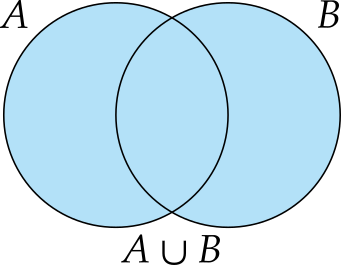
\includegraphics[width=6cm,height=\textheight]{./img/teoria-conjuntos/union.png}

}

\caption{Unión de conjuntos}

\end{figure}

\leavevmode\vadjust pre{\hypertarget{def-interseccion-conjuntos}{}}%
\begin{definition}[Intersección]\label{def-interseccion-conjuntos}

Dados dos conjuntos \(A\) y \(B\), se llama \emph{intersección} de \(A\)
y \(B\), y se denota \(A\cap B\), al conjunto de todos los elementos
comunes a \(A\) y \(B\).

\[A\cap B = \{x\,:\, x\in A\mbox{ y }x\in B\}.\]

\end{definition}

\begin{figure}

{\centering 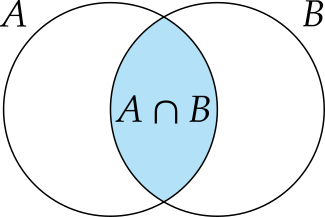
\includegraphics[width=6cm,height=\textheight]{./img/teoria-conjuntos/interseccion.png}

}

\caption{Intersección de conjuntos}

\end{figure}

\leavevmode\vadjust pre{\hypertarget{def-complemento-conjuntos}{}}%
\begin{definition}[Complemento]\label{def-complemento-conjuntos}

Dado un conjunto \(A\subset \Omega\), se llama \emph{complemento} de
\(A\) con respecto a \(\Omega\), y se denota \(\overline A\), al
conjunto de todos los elementos de \(\Omega\) que no pertenecen a \(A\).

\[\overline A = \{x\in \Omega\,:\, x\not\in A\}.\]

\end{definition}

\begin{figure}

{\centering 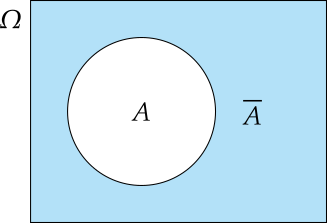
\includegraphics[width=7cm,height=\textheight]{./img/teoria-conjuntos/complemento.png}

}

\caption{Complemento de un conjunto}

\end{figure}

\leavevmode\vadjust pre{\hypertarget{def-diferencia-conjuntos}{}}%
\begin{definition}[Diferencia]\label{def-diferencia-conjuntos}

Dados dos conjuntos \(A\) y \(B\), se llama \emph{diferencia} de \(A\) y
\(B\), y se denota \(A-B\), al conjunto formado por los elementos de
\(A\) que no pertenecen a \(B\), es decir,

\[A-B = \{x\,:\, x\in A\mbox{ y }x\not\in B\}.\]

\end{definition}

\begin{figure}

{\centering 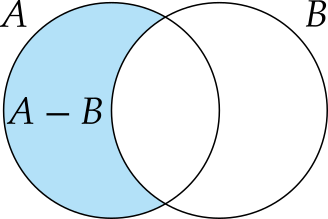
\includegraphics[width=6cm,height=\textheight]{./img/teoria-conjuntos/diferencia.png}

}

\caption{Diferencia de conjuntos}

\end{figure}

\leavevmode\vadjust pre{\hypertarget{def-diferencia-simetrica-conjuntos}{}}%
\begin{definition}[Diferencia
simétrica]\label{def-diferencia-simetrica-conjuntos}

Dados dos conjuntos \(A\) y \(B\), se llama \emph{diferencia simétrica}
de \(A\) y \(B\), y se denota \(A\triangle B\), al conjunto formado por
los elementos que pertenecen a \(A\) o \(B\), pero no a ambos a la vez,
es decir,

\begin{align*}
A\triangle B &= \{x\,:\, x\in A-B\mbox{ o }x\in B-A\}\\ 
&= (A-B) \cup (B-A) = (A\cup B)-(A\cap B)
\end{align*}

\end{definition}

\begin{figure}

{\centering 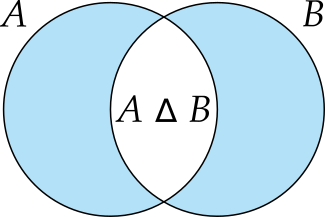
\includegraphics[width=6cm,height=\textheight]{./img/teoria-conjuntos/diferencia-simetrica.png}

}

\caption{Diferencia simétrica de conjuntos}

\end{figure}

\leavevmode\vadjust pre{\hypertarget{exm-operaciones-conjuntos}{}}%
\begin{example}[]\label{exm-operaciones-conjuntos}

Dado el conjunto de los números que contiene un dado,
\(\Omega=\{1,2,3,4,5,6\}\) y sus subconjuntos \(A=\{2,4,6\}\) y
\(B=\{1,2,3,4\}\),

\begin{itemize}
\tightlist
\item
  La unión de \(A\) y \(B\) es \(A\cup B=\{1,2,3,4,6\}\).
\item
  La intersección de \(A\) y \(B\) es \(A\cap B=\{2,4\}\).
\item
  El contrario de \(A\) con respecto a \(\Omega\) es
  \(\overline A=\{1,3,5\}\).
\item
  La diferencia de \(A\) y \(B\) es \(A-B=\{6\}\), y la diferencia de
  \(B\) y \(A\) es \(B-A=\{1,3\}\).
\item
  La diferencia simétrica de \(A\) y \(B\) es
  \(A\triangle B = \{1, 3, 6\}\).
\end{itemize}

\end{example}

\leavevmode\vadjust pre{\hypertarget{prp-propiedades-conjuntos}{}}%
\begin{proposition}[]\label{prp-propiedades-conjuntos}

Dado un conjunto universo \(\Omega\) y los conjuntos
\(A,B,C\subseteq \Omega\), se cumplen las siguientes propiedades:

\begin{enumerate}
\def\labelenumi{\arabic{enumi}.}
\tightlist
\item
  Idempotencia: \(A\cup A=A\) y \(A\cap A=A\).
\item
  Conmutativa: \(A\cup B=B\cup A\) y \(A\cap B = B\cap A\).
\item
  Asociativa: \((A\cup B)\cup C = A\cup (B\cup C)\) y
  \((A\cap B)\cap C = A\cap (B\cap C)\).
\item
  Distributiva: \((A\cup B)\cap C = (A\cap C)\cup (B\cap C)\) y
  \((A\cap B)\cup C = (A\cup C)\cap (B\cup C)\).
\item
  Elemento neutro: \(A\cup \emptyset=A\) y \(A\cap \Omega=A\).
\item
  Elemento absorvente: \(A\cup \Omega=\Omega\) y
  \(A\cap \emptyset=\emptyset\).
\item
  Elemento simétrico complementario: \(A\cup \overline A = E\) y
  \(A\cap \overline A= \emptyset\).
\item
  Doble complemento: \(\overline{\overline A} = A\).
\item
  Leyes de Morgan: \(\overline{A\cup B} = \overline A\cap \overline B\)
  y \(\overline{A\cap B} = \overline A\cup \overline B\).
\item
  \(A\cap B\subseteq A\cup B\).
\item
  \(A-B = A \cap \overline B\).
\item
  \(A-B\subseteq A\) y \(B-A\subseteq B\).
\item
  \(A\triangle B = (A\cup B) - (A\cap B)\).
\item
  \(\overline \Omega = \emptyset\) y \(\overline \emptyset = \Omega\).
\end{enumerate}

\end{proposition}

\leavevmode\vadjust pre{\hypertarget{def-conjuntos-disjuntos}{}}%
\begin{definition}[Conjuntos disjuntos]\label{def-conjuntos-disjuntos}

Dados dos conjuntos \(A\) y \(B\), se dice que son \emph{disjuntos} si
no tienen ningún elemento en común, es decir, \(A\cap B=\emptyset\).

\end{definition}

\leavevmode\vadjust pre{\hypertarget{def-conjunto-potencia}{}}%
\begin{definition}[Conjunto potencia]\label{def-conjunto-potencia}

Dado un conjunto \(A\), se llama \emph{conjunto potencia} o
\emph{conjunto de las partes} de \(A\), y se denota \(\mathcal{P}(A)\),
al conjunto de todos los subconjuntos de \(A\), es decir,

\[\mathcal{P}(A) = \{ X \, : \,  X \subseteq A \}\]

\end{definition}

\leavevmode\vadjust pre{\hypertarget{exm-conjunto-potencia}{}}%
\begin{example}[]\label{exm-conjunto-potencia}

El conjunto potencia del conjunto \(A=\{1, 2, 3\}\) es

\end{example}

\[\mathcal{P}(A)=\{\emptyset, \{1\}, \{2\}, \{3\}, \{1,2\}, \{1,3\}, \{2,3\}, \{1,2,3\}\}\]

\hypertarget{relaciones-entre-conjuntos}{%
\section{Relaciones entre conjuntos}\label{relaciones-entre-conjuntos}}

\leavevmode\vadjust pre{\hypertarget{def-par-ordenado}{}}%
\begin{definition}[Par ordenado]\label{def-par-ordenado}

Dados dos elementos \(a\) y \(b\) se define el \emph{par ordenado}
\((a,b)\) como \[ (a,b) = \{\{a\}, \{a,b\}\} \]

De manera más general, se define una \emph{\(n\)-tupla ordenada} como
\[(a_1, a_2, \ldots, a_n) = ((a_1, a_2, \ldots, a_{n-1}), a_n)\]

\end{definition}

De forma mas informal, decimos que \((a,b)\) es un par ordenado si el
primer elemento (\(a\)) se distingue del segundo elemento (\(b\)). Por
eso, se tiene que \((a,b) \neq (b,a)\), mientras que para conjuntos
\(\{a,b\}=\{b,a\}\).

\leavevmode\vadjust pre{\hypertarget{def-producto-cartesiano}{}}%
\begin{definition}[Producto cartesiano]\label{def-producto-cartesiano}

Dados dos conjuntos \(A\) y \(B\), se llama \emph{producto cartesiano}
de \(A\) y \(B\), y se denota \(A\times B\), al conjunto de los pares
ordenados

\[A \times B = \{ (a,b) \, : \,  a \in A \mbox{ y } b \in B \}\]

De manera más general, si se tienen \(n\) conjuntos
\(A_1, A_2, \ldots, A_n\), el \emph{producto cartesiano generalizado} es

\[A_1 \times A_2 \times \ldots \times A_n = \{ (a_1, \ldots, a_n) \, :\, a_i \in A_i\ \forall i=1, \ldots n\}\]

\end{definition}

\leavevmode\vadjust pre{\hypertarget{def-relacion-binaria}{}}%
\begin{definition}[Relación binaria]\label{def-relacion-binaria}

Dados dos conjuntos \(A\) y \(B\), se dice que \(R\) es una
\emph{relación binaria} sobre \(A\) y \(B\) si es un subconjunto del
producto cartesiano de \(A\) y \(B\), es decir,
\[ R \subseteq A \times B \]

Si \(A\) y \(B\) son el mismo conjunto, se dice que \(R\) es una
\emph{relación binaria homogénea}.

\end{definition}

Cuando un par ordenado pertenece a una relación, \((a,b)\in R\), también
se suele escribir \(aRb\).

Dependiendo de las propiedades que cumpla una relación tenemos los
siguientes tipos de relaciones:

\begin{itemize}
\tightlist
\item
  \textbf{Reflexiva}: \(\forall a \in A, (a,a) \in R\)
\item
  \textbf{Irreflexiva}: \(\forall a \in A, (a,a) \not\in R\).
\item
  \textbf{Simétrica}: \(\forall a, b \in A\), si \((a,b) \in R\),
  entonces \((b,a) \in R\).
\item
  \textbf{Asimétrica}: \(\forall a, b \in A\), si \((a,b) \in R\),
  entonces \((b,a) \not\in R\).
\item
  \textbf{Antisimétrica}: \(\forall a, b \in A\), si \((a,b) \in R\) y
  \((b,a) \in R\), entonces \(a = b\).
\item
  \textbf{Transitiva}: \(\forall a, b, c \in A\), si \((a,b) \in R\) y
  \((b,c) \in R\), entonces \((a,c) \in R\).
\item
  \textbf{Total}: \(\forall a, b \in A\), \((a,b) \in R\) o
  \((b,a) \in R\).
\end{itemize}

\leavevmode\vadjust pre{\hypertarget{def-relacion-equivalencia}{}}%
\begin{definition}[Relación de
equivalencia]\label{def-relacion-equivalencia}

Dado un conjunto \(A\) y una relación homogénea
\(R \subseteq A \times A\), se dice que \(R\) es una \emph{relación de
equivalencia}, y se denota \((A, \sim)\), si es que cumple que \(R\) es
reflexiva, simétrica y transitiva, es decir, si cumple las propiedades

\begin{itemize}
\tightlist
\item
  \emph{Reflexiva:} \(\forall a \in A, a \sim a\).
\item
  \emph{Simétrica:} \(\forall a, b \in A\), si \(a\sim b\) entonces
  \(b\sim a\).
\item
  \emph{Transitiva:} \(\forall a, b, c \in A\), si \(a\sim b\) y
  \(b\sim c\), entonces \(a\sim c\).
\end{itemize}

\end{definition}

\leavevmode\vadjust pre{\hypertarget{exm-relacion-equivalencia}{}}%
\begin{example}[]\label{exm-relacion-equivalencia}

Ya hemos visto que la relación de igualdad matemática entre los
elementos de un conjunto es una relación de equivalencia.

\end{example}

\leavevmode\vadjust pre{\hypertarget{def-relacion-orden}{}}%
\begin{definition}[Relación de orden]\label{def-relacion-orden}

Dado un conjunto \(A\) y una relación homogénea
\(\preceq \subseteq A \times A\), se dice que \(\preceq\) es una
\emph{relación de orden}, si es una relación reflexiva, antisimétrica y
transitiva, es decir, si cumple las propiedades

\begin{itemize}
\tightlist
\item
  \emph{Reflexiva:} \(\forall a \in A, a \preceq a\).
\item
  \emph{Antisimétrica:} \(\forall a, b \in A\), si \(a\preceq b\) y
  \(b\preceq a\), entonces \(a = b\).
\item
  \emph{Transitiva:} \(\forall a, b, c \in A\), si \(a\preceq b\) y
  \(b\preceq c\), entonces \(a\preceq c\).
\end{itemize}

\end{definition}

\leavevmode\vadjust pre{\hypertarget{def-relacion-orden-parcial}{}}%
\begin{definition}[Relación de orden
parcial]\label{def-relacion-orden-parcial}

Dado un conjunto \(A\) y una relación homogénea
\(\preceq \subseteq A \times A\), se dice que \(\preceq\) es una
\emph{relación de orden parcial}, si es una relación de orden y al menos
dos elementos de \(A\) están relacionados mediante \(\preceq\), es
decir,

\[\exists x, y\in A,\ x\preceq y \mbox{ o } y\preceq x.\]

Al conjunto \(A\) con la relación de orden parcial \(\preceq\) se le
llama \emph{conjunto parcialmente ordenado}, y se denota
\((A,\preceq)\).

\end{definition}

\leavevmode\vadjust pre{\hypertarget{exm-relacion-orden-parcial}{}}%
\begin{example}[]\label{exm-relacion-orden-parcial}

El conjunto potencia de un conjunto \(A\) con la relación de inclusión
es un conjunto parcialmente ordenado \((\mathcal{P}(A),\subseteq)\).

\end{example}

\leavevmode\vadjust pre{\hypertarget{def-relacion-orden-total}{}}%
\begin{definition}[Relación de orden
total]\label{def-relacion-orden-total}

Dado un conjunto \(A\) y una relación homogénea
\(\preceq \subseteq A \times A\), se dice que \(\preceq\) es una
\emph{relación de orden total}, si es una relación de orden y todos los
elementos de \(A\) se relacionan entre sí mediante \(\preceq\), es
decir,

\[\forall x, y\in A,\ x\preceq y \mbox{ o } y \preceq x.\]

Al conjunto \(A\) con la relación de orden total \(\preceq\) se le llama
\emph{conjunto totalmente ordenado}, y se denota \((A,\preceq)\).

\end{definition}

\leavevmode\vadjust pre{\hypertarget{exm-relacion-orden-total}{}}%
\begin{example}[]\label{exm-relacion-orden-total}

La relación de orden de los números naturales \((\mathbb{N},\leq)\) es
un orden totalmente ordenado. Sin embargo, la relación de inclusión en
el conjunto potencia de un conjunto \(A\) (\(\mathcal{P}(A),\subseteq\))
no es un orden parcialmente ordenado, ya que dados dos elementos
\(a\neq b\) de \(A\), se cumple que \(\{a\}\subsetneq \{b\}\) y
\(\{b\}\subsetneq \{a\}\).

\end{example}

\hypertarget{cotas-y-extremos}{%
\section{Cotas y extremos}\label{cotas-y-extremos}}

\leavevmode\vadjust pre{\hypertarget{def-cota-superior-conjunto}{}}%
\begin{definition}[Cota superior]\label{def-cota-superior-conjunto}

Dado un subconjunto con una relación de orden parcial \((A,\preceq)\) y
un subconjunto \(B\subseteq A\), se dice que un elemento \(c\in A\) es
una \emph{cota superior} de \(B\), si todos los elementos de \(B\) son
menores o iguales a \(c\) según la relación de orden, es decir,

\[\forall x \in B, x\preceq c.\]

\end{definition}

\leavevmode\vadjust pre{\hypertarget{def-cota-inferior-conjunto}{}}%
\begin{definition}[Cota inferior]\label{def-cota-inferior-conjunto}

Dado un subconjunto con una relación de orden parcial \((A,\preceq)\) y
un subconjunto \(B\subseteq A\), se dice que un elemento \(c\in A\) es
una \emph{cota inferior} de \(B\), si todos los elementos de \(B\) son
mayores o iguales a \(c\) según la relación de orden, es decir,

\[\forall x \in B, c\preceq x.\]

\end{definition}

\leavevmode\vadjust pre{\hypertarget{def-maximo-conjunto}{}}%
\begin{definition}[Máximo]\label{def-maximo-conjunto}

Dado un conjunto con una relación de orden parcial \((A,\preceq)\), se
dice que un elemento \(m\in A\) es un \emph{máximo} de \(A\), si
cualquier otro elemento de \(A\) es mayor o igual que él según la
relación de orden, es decir,

\[\forall x \in A, x\preceq m.\]

\end{definition}

\leavevmode\vadjust pre{\hypertarget{def-minimo-conjunto}{}}%
\begin{definition}[Mínimo]\label{def-minimo-conjunto}

Dado un conjunto con una relación de orden parcial \((A,\preceq)\), se
dice que un elemento \(m\in A\) es un \emph{mínimo} de \(A\), si y
cualquier otro elemento de \(A\) es menor o igual que él según la
relación de orden, es decir,

\[\forall x \in A, m\preceq x.\]

\end{definition}

\leavevmode\vadjust pre{\hypertarget{thm-unicidad-extremos}{}}%
\begin{theorem}[Unicidad de los extremos]\label{thm-unicidad-extremos}

Dado un conjunto con una relación de orden parcial \((A,\preceq)\), si
existe el máximo de \(A\) entonces es único. Lo mismo es cierto para el
mínimo.

\end{theorem}

\begin{tcolorbox}[enhanced jigsaw, left=2mm, colframe=quarto-callout-note-color-frame, rightrule=.15mm, opacityback=0, leftrule=.75mm, colback=white, toprule=.15mm, breakable, bottomtitle=1mm, titlerule=0mm, toptitle=1mm, arc=.35mm, title=\textcolor{quarto-callout-note-color}{\faInfo}\hspace{0.5em}{Demostración}, bottomrule=.15mm, opacitybacktitle=0.6, coltitle=black, colbacktitle=quarto-callout-note-color!10!white]

\begin{proof}

Supongamos que el conjunto \(A\) tienen dos máximos \(m_1\neq m_2\).
Puesto que \(m_1\) es un máximo de \(A\), se cumple que
\(\forall x \in A, x\preceq m_1.\) y, en particular, \(m_2\preceq m_1\).
Del mismo modo, como \(m_2\) es un máximo de \(A\), se cumple que
\(\forall x \in A, x\preceq m_2.\) y, en particular, \(m_1\preceq m_2\).

Así pues, se tiene que

\[m_2\preceq m_1 \mbox{ y } m_1\preceq m_2,\]

pero como \(\preceq\) es un orden parcial, por la propiedad
antisimétrica se concluye que \(m_1=m_2\), por lo que el máximo es
único.

De manera análoga se puede probar que el mínimo es único.

\end{proof}

\end{tcolorbox}

Dado que el máximo y mínimo de un conjunto, cuando existen, son únicos,
es común referirse a ellos como \(max\) y \(min\) respectivamente.
Obsérvese, no obstante, que un conjunto puede no tener máximo o mínimo.

\leavevmode\vadjust pre{\hypertarget{def-supremo-conjunto}{}}%
\begin{definition}[Supremo]\label{def-supremo-conjunto}

Dado un subconjunto con una relación de orden parcial \((A,\preceq)\) y
un subconjunto \(B\subseteq A\), se llama \emph{supremo} de \(B\) y se
denota \(\sup(B)\) a la menor de las cotas superiores de \(B\).

\end{definition}

\leavevmode\vadjust pre{\hypertarget{def-infimo-conjunto}{}}%
\begin{definition}[Ínfimo]\label{def-infimo-conjunto}

Dado un subconjunto con una relación de orden parcial \((A,\preceq)\) y
un subconjunto \(B\subseteq A\), se llama \emph{ínfimo} de \(B\) y se
denota \(\inf(B)\) a la mayor de las cotas inferiores de \(B\).

\end{definition}

Obsérvese que un conjunto puede no tener supremo o ínfimo.

\leavevmode\vadjust pre{\hypertarget{exm-supremo-infimo-maximo-minimo}{}}%
\begin{example}[]\label{exm-supremo-infimo-maximo-minimo}

Si se toma el conjunto de los números naturales con la relación de orden
total \((\mathbb{N},\leq)\), para el conjunto
\(B=\{1, 2, 3\}\subseteq \mathbb{N}\) se tiene que cualquier
\(x\in\mathbb{N}\) tal que \(3\leq x\) es una cota superior de \(B\),
por tanto \(3\) es el supremo de \(B\), y además es un máximo puesto que
\(3\in B\).

Por otro lado, si se considera el conjunto de los números reales con la
relación de orden total \((\mathbb{R},\leq)\), para el intervalo
\((0,1)\) se tiene que cualquier \(x\in\mathbb{R}\) tal que \(x\leq 0\)
es una cota inferior y \(x\in\mathbb{R}\) tal que \(1\leq x\) es una
cota superior, de modo que \(0\) es el ínfimo y \(1\) el supremo. Sin
embargo, este conjunto no tiene mínimo ni tampoco máximo puesto que
\(0\not\in (0,1)\) y \(1\not\in (0,1)\).

Finalmente, si se considera el conjunto de los números enteros con la
relación de orden total \((\mathbb{Z},\leq)\), para el conjunto
\(B=\{x\in\mathbb{Z}: x \mbox{ es par}\}\), no existen cotas superiores
ni inferiores, y por tanto tampoco tiene supremo, ínfimo, máximo ni
mínimo.

\end{example}

\hypertarget{funciones}{%
\section{Funciones}\label{funciones}}

El concepto de función es uno de los más importantes en el Análisis
Matemático, ya que muchos de los fenómenos naturales en los que una
magnitud depende de otra se modelizan mediante funciones.

\leavevmode\vadjust pre{\hypertarget{def-funcion}{}}%
\begin{definition}[Función]\label{def-funcion}

Se dice que una relación binaria \(f \subseteq A \times B\), con \(A\) y
\(B\) conjuntos no vacios, es una \emph{función} o \emph{aplicación}, y
se denota \(f:A\rightarrow B\), si \(f\) no contiene dos pares ordenados
distintos con la misma primera componente, es decir,

\[\forall a \in A, \forall b_1, b_2 \in B, \mbox{ si } (a,b_1) \in f \mbox{ y } (a,b_2) \in f, \mbox{ entonces } b_1 = b_2.\]

\end{definition}

Es habitual representar los pares de una función con la notación
\(y=f(x)\) donde \(x\) es la primera componente del par e \(y\) la
segunda.

\leavevmode\vadjust pre{\hypertarget{exm-funcion}{}}%
\begin{example}[]\label{exm-funcion}

La relación binaria \(f=\{(1,a), (2,c), (3,c), (4,b)\}\) es una función,
pero la relación \(g=\{(1,a), (2,c), (3,c), (2,b)\}\) no lo es porque
existen dos pares cuya primera componente es \(2\). Del mismo modo la
función raíz cuadrada \(y=f(x)=\sqrt{x}\) no es una función en el
conjunto de los números reales, ya que, por ejemplo \(\sqrt{1}=\pm 1\).

\end{example}

\begin{figure}

\begin{minipage}[t]{0.50\linewidth}

{\centering 

\raisebox{-\height}{

\begin{tikzpicture}[scale=1.5,every node/.style={transform shape}]
\filldraw[fill=blue!20, draw=blue!60] (-1.5,0) ellipse (1cm and 1.5cm);
\filldraw[fill=red!20, draw=red!60] (1.5,0) ellipse (1cm and 1.5cm);

    \node at (-1.5,1.8) {$A$};
    \node at (1.5,1.8) {$B$};

    \node (x1) at (-1.5,0.9) {$1$};
    \node (x2) at (-1.5,0.3) {$2$};
    \node (x3) at (-1.5,-0.3) {$3$};
    \node (x4) at (-1.5,-0.9) {$4$};
    \node (y1) at (1.5,0.9) {$a$};
    \node (y2) at (1.5,0.3) {$b$};
    \node (y3) at (1.5,-0.3) {$c$};
    \node (y4) at (1.5,-0.9) {$d$};

    % draw the arrows
    \draw[-stealth] (x1) -- (y4);
    \draw[-stealth] (x2) -- (y3);
    \draw[-stealth] (x3) -- (y1);
    \draw[-stealth] (x4) -- (y3);

\end{tikzpicture}

}

\caption{Ejemplo de función}

}

\end{minipage}%
%
\begin{minipage}[t]{0.50\linewidth}

{\centering 

\raisebox{-\height}{

\begin{tikzpicture}[scale=1,every node/.style={transform shape}]
\filldraw[fill=blue!20, draw=blue!60] (-1.5,0) ellipse (1cm and 1.5cm);
\filldraw[fill=red!20, draw=red!60] (1.5,0) ellipse (1cm and 1.5cm);

    \node at (-1.5,1.8) {$A$};
    \node at (1.5,1.8) {$B$};

    \node (x1) at (-1.5,0.6) {$1$};
    \node (x2) at (-1.5,0.0) {$2$};
    \node (x3) at (-1.5,-0.6) {$3$};
   % \node (x4) at (-1.5,-0.9) {$4$};
    \node (y1) at (1.5,0.9) {$a$};
    \node (y2) at (1.5,0.3) {$b$};
    \node (y3) at (1.5,-0.3) {$c$};
    \node (y4) at (1.5,-0.9) {$d$};

    % draw the arrows
    \draw[-stealth] (x1) -- (y4);
    \draw[-stealth] (x2) -- (y2);
    \draw[-stealth] (x3) -- (y1);
    \draw[-stealth] (x3) -- (y3);
    %\draw[-stealth] (x4) -- (y3);

\end{tikzpicture}

}

\caption{Ejemplo de no función}

}

\end{minipage}%

\end{figure}

\leavevmode\vadjust pre{\hypertarget{def-dominio-funcion}{}}%
\begin{definition}[Dominio]\label{def-dominio-funcion}

Dada una función \(f:A\rightarrow B\), se llama \emph{dominio} de \(f\),
y se denota \(\operatorname{Dom}(f)\) al conjunto de las primeras
componentes de los pares de \(f\), es decir,

\[\operatorname{Dom}(f) = \{a\in A: \exists b\in B, (a,b)\in f\}\]

\end{definition}

\leavevmode\vadjust pre{\hypertarget{def-imagen-funcion}{}}%
\begin{definition}[Imagen]\label{def-imagen-funcion}

Dada una función \(f:A\rightarrow B\), se llama \emph{imagen} de \(f\),
y se denota \(\operatorname{Im}(f)\) al conjunto de las segundas
componentes de los pares de \(f\), es decir,

\[\operatorname{Im}(f) = \{b\in B: \exists a\in A, (a,b)\in f\}\]

\end{definition}

\leavevmode\vadjust pre{\hypertarget{def-funcion-inyectiva}{}}%
\begin{definition}[Función inyectiva]\label{def-funcion-inyectiva}

Dada una función \(f:A\rightarrow B\), se dice que \(f\) es
\emph{inyectiva} si no existen dos elementos de \(A\) con la misma
imagen, es decir,

\[\forall a_1, a_2 \in A, \mbox{ si } f(a_1) = f(a_2), \mbox{ entonces } a_1 = a_2.\]

\end{definition}

\leavevmode\vadjust pre{\hypertarget{def-funcion-sobreyectiva}{}}%
\begin{definition}[Función sobreyectiva]\label{def-funcion-sobreyectiva}

Dada una función \(f:A\rightarrow B\), se dice que \(f\) es
\emph{sobreyectiva} si todo elemento de \(B\) tiene una preimagen (está
relacionado con algún elemento de \(A\) mediante \(f\)), es decir,

\[\forall b \in B, \exists a\in A, f(a) = b.\]

\end{definition}

\leavevmode\vadjust pre{\hypertarget{def-funcion-biyectiva}{}}%
\begin{definition}[Función biyectiva]\label{def-funcion-biyectiva}

Dada una función \(f:A\rightarrow B\), se dice que \(f\) es
\emph{biyectiva}, si \(f\) es, a la vez, inyectiva y sobreyectiva.

\end{definition}

\begin{figure}

\begin{minipage}[t]{0.50\linewidth}

{\centering 

\raisebox{-\height}{

\begin{tikzpicture}[scale=1.5,every node/.style={transform shape}]
\filldraw[fill=blue!20, draw=blue!60] (-1.5,0) ellipse (1cm and 1.5cm);
\filldraw[fill=red!20, draw=red!60] (1.5,0) ellipse (1cm and 1.5cm);

    \node at (-1.5,1.8) {$A$};
    \node at (1.5,1.8) {$B$};

    \node (x1) at (-1.5,0.6) {$1$};
    \node (x2) at (-1.5,0) {$2$};
    \node (x3) at (-1.5,-0.6) {$3$};
%    \node (x4) at (-1.5,-0.9) {$4$};
    \node (y1) at (1.5,0.9) {$a$};
    \node (y2) at (1.5,0.3) {$b$};
    \node (y3) at (1.5,-0.3) {$c$};
    \node (y4) at (1.5,-0.9) {$d$};

    % draw the arrows
    \draw[-stealth] (x1) -- (y4);
    \draw[-stealth] (x2) -- (y2);
    \draw[-stealth] (x3) -- (y1);
    %\draw[-stealth] (x4) -- (y3);

\end{tikzpicture}

}

\caption{Función inyectiva y no sobreyectiva}

}

\end{minipage}%
%
\begin{minipage}[t]{0.50\linewidth}

{\centering 

\raisebox{-\height}{

\begin{tikzpicture}[scale=1,every node/.style={transform shape}]
\filldraw[fill=blue!20, draw=blue!60] (-1.5,0) ellipse (1cm and 1.5cm);
\filldraw[fill=red!20, draw=red!60] (1.5,0) ellipse (1cm and 1.5cm);

    \node at (-1.5,1.8) {$A$};
    \node at (1.5,1.8) {$B$};

    \node (x1) at (-1.5,0.9) {$1$};
    \node (x2) at (-1.5,0.3) {$2$};
    \node (x3) at (-1.5,-0.3) {$3$};
    \node (x4) at (-1.5,-0.9) {$4$};
    \node (y1) at (1.5,0.6) {$a$};
    \node (y2) at (1.5,0) {$b$};
    \node (y3) at (1.5,-0.6) {$c$};
    %\node (y4) at (1.5,-0.9) {$d$};

    % draw the arrows
    \draw[-stealth] (x2) -- (y3);
    \draw[-stealth] (x1) -- (y2);
    \draw[-stealth] (x3) -- (y1);
    \draw[-stealth] (x4) -- (y3);

\end{tikzpicture}

}

\caption{Función sobreyectiva y no inyectiva}

}

\end{minipage}%
\newline
\begin{minipage}[t]{0.50\linewidth}

{\centering 

\raisebox{-\height}{

\begin{tikzpicture}[scale=1.5,every node/.style={transform shape}]
\filldraw[fill=blue!20, draw=blue!60] (-1.5,0) ellipse (1cm and 1.5cm);
\filldraw[fill=red!20, draw=red!60] (1.5,0) ellipse (1cm and 1.5cm);

    \node at (-1.5,1.8) {$A$};
    \node at (1.5,1.8) {$B$};

    \node (x1) at (-1.5,0.9) {$1$};
    \node (x2) at (-1.5,0.3) {$2$};
    \node (x3) at (-1.5,-0.3) {$3$};
    \node (x4) at (-1.5,-0.9) {$4$};
    \node (y1) at (1.5,0.9) {$a$};
    \node (y2) at (1.5,0.3) {$b$};
    \node (y3) at (1.5,-0.3) {$c$};
    \node (y4) at (1.5,-0.9) {$d$};

    % draw the arrows
    \draw[-stealth] (x1) -- (y4);
    \draw[-stealth] (x2) -- (y2);
    \draw[-stealth] (x3) -- (y1);
    \draw[-stealth] (x4) -- (y3);

\end{tikzpicture}

}

\caption{Función biyectiva}

}

\end{minipage}%
%
\begin{minipage}[t]{0.50\linewidth}

{\centering 

\raisebox{-\height}{

\begin{tikzpicture}[scale=1.5,every node/.style={transform shape}]
\filldraw[fill=blue!20, draw=blue!60] (-1.5,0) ellipse (1cm and 1.5cm);
\filldraw[fill=red!20, draw=red!60] (1.5,0) ellipse (1cm and 1.5cm);

    \node at (-1.5,1.8) {$A$};
    \node at (1.5,1.8) {$B$};

    \node (x1) at (-1.5,0.9) {$1$};
    \node (x2) at (-1.5,0.3) {$2$};
    \node (x3) at (-1.5,-0.3) {$3$};
    \node (x4) at (-1.5,-0.9) {$4$};
    \node (y1) at (1.5,0.9) {$a$};
    \node (y2) at (1.5,0.3) {$b$};
    \node (y3) at (1.5,-0.3) {$c$};
    \node (y4) at (1.5,-0.9) {$d$};

    % draw the arrows
    \draw[-stealth] (x1) -- (y4);
    \draw[-stealth] (x2) -- (y3);
    \draw[-stealth] (x3) -- (y1);
    \draw[-stealth] (x4) -- (y3);

\end{tikzpicture}

}

\caption{Función no inyectiva y no sobreyectiva}

}

\end{minipage}%

\end{figure}

\leavevmode\vadjust pre{\hypertarget{def-funcion-identidad}{}}%
\begin{definition}[Función identidad]\label{def-funcion-identidad}

Dado un conjunto \(A\), se llama \emph{función identidad} de \(A\), y se
denota \(\operatorname{id}_A:A\rightarrow A\), a la función que empareja
cada elemento de \(A\) consigo mismo, es decir,

\[\operatorname{id}_A (a) = a, \forall a\in A.\]

\end{definition}

\leavevmode\vadjust pre{\hypertarget{def-funcion-inversa}{}}%
\begin{definition}[Función inversa]\label{def-funcion-inversa}

Dada una función \(f:A\rightarrow B\), se llama \emph{función inversa}
de \(f\), y se denota \(f^{-1}:B\rightarrow A\), a la función que
resulta de revertir el orden de los pares de \(f\), es decir,

\[f^{-1} = \{ (b,a) : (a,b) \in f \}.\]

\end{definition}

Obsérvese que para que exista la función inversa de \(f\), \(f\) debe
ser inyectiva.

En muchas ocasiones, el valor de salida de una función se puede utilizar
como la entrada de otra función, concatenando la aplicación de las dos
funciones.

\leavevmode\vadjust pre{\hypertarget{def-composicion-funciones}{}}%
\begin{definition}[Composición de
funciones]\label{def-composicion-funciones}

Dadas dos funciones \(f:A\rightarrow B\) y \(g:C\rightarrow D\), tales
que \(\operatorname{Im}(f)\subseteq \operatorname{Dom}(g)\), se llama
\emph{composición} de \(f\) con \(g\), y se denota
\(g\circ f:A\rightarrow D\), a la funcion que a cada elemento del
dominio de \(A\) le asocia el elemento que resulta de aplicar \(g\) a la
imagen de \(a\) mediante \(f\), es decir,

\[g\circ f(a) = g(f(a)), \forall a\in A.\]

\end{definition}

\leavevmode\vadjust pre{\hypertarget{prp-composicion-inversa}{}}%
\begin{proposition}[]\label{prp-composicion-inversa}

Dada una función \(f:A\rightarrow B\), si existe \$\^{}\{-1\}, entonces
\(f\circ f^{-1} = \operatorname{id}_A\) y
\(f^{-1}\circ f = \operatorname{id}_B\).

\end{proposition}

\hypertarget{cardinalidad-de-un-conjunto}{%
\section{Cardinalidad de un
conjunto}\label{cardinalidad-de-un-conjunto}}

\leavevmode\vadjust pre{\hypertarget{def-cardinal-conjunto}{}}%
\begin{definition}[Cardinal]\label{def-cardinal-conjunto}

Dado un conjunto \(A\), se llama \emph{cardinal} de \(A\), y se denota
\(|A|\), al número de elementos de \(A\).

\end{definition}

De manera informal, se puede decir Que el cardinal de un conjunto es su
tamaño.

\leavevmode\vadjust pre{\hypertarget{exm-cardinal}{}}%
\begin{example}[]\label{exm-cardinal}

El cardinal del conjunto \(A=\{a, b, c\}\) es \(|A|=3\).

\end{example}

\leavevmode\vadjust pre{\hypertarget{prp-cardinal-conjunto-potencia}{}}%
\begin{proposition}[]\label{prp-cardinal-conjunto-potencia}

El cardinal del conjunto potencia de un conjunto \(A\) es
\(|\mathcal{P}(A)| = 2^{|A|}\).

\end{proposition}

\begin{tcolorbox}[enhanced jigsaw, left=2mm, colframe=quarto-callout-note-color-frame, rightrule=.15mm, opacityback=0, leftrule=.75mm, colback=white, toprule=.15mm, breakable, bottomtitle=1mm, titlerule=0mm, toptitle=1mm, arc=.35mm, title=\textcolor{quarto-callout-note-color}{\faInfo}\hspace{0.5em}{Demostración}, bottomrule=.15mm, opacitybacktitle=0.6, coltitle=black, colbacktitle=quarto-callout-note-color!10!white]

\begin{proof}

Se puede dar una prueba mediante coeficientes binomiales. Si \(A\) tiene
\(n\) elementos, es decir, \(|\)A\(|=n\), el número de subconjuntos
distintos con \(k\) elementos es igual al número combinatorio
\[\binom{n}{k}=\frac{n!}{k!(n-k)!}.\]

Como un subconjunto de \(A\) puede tener desde \(0\) hasta \(n\)
elementos, en total, el número de posibles subconjuntos de \(A\) será

\[|\mathcal{P}(A)|=\binom{n}{0}+\binom{n}{1}+\cdots + \binom{n}{n} = \sum_{k=0}^n \binom{n}{k},\]

y según el teorema del binomio de Newton se tiene que

\[\sum_{k=0}^n \binom{n}{k}=2^n = 2^{|A|}.\]

\end{proof}

\end{tcolorbox}

\leavevmode\vadjust pre{\hypertarget{def-conjuntos-equipotentes}{}}%
\begin{definition}[Conjuntos
equipotentes]\label{def-conjuntos-equipotentes}

Se dice que dos conjuntos \(A\) y \(B\) son \emph{equipotentes}, y se
denota \(A\approx B\), si tienen la misma cantidad de elementos, es
decir, si \(|A| = |B|\).

\end{definition}

\leavevmode\vadjust pre{\hypertarget{prp-biyeccion-conjuntos-equipotentes}{}}%
\begin{proposition}[]\label{prp-biyeccion-conjuntos-equipotentes}

Dos conjuntos \(A\) y \(B\) son equipotentes si y solo si cada elemento
de \(A\) puede emparejarse con uno de \(B\), de manera que todos los
elementos de \(B\) sean pareja de uno de \(A\) y solo de uno, es decir,
existe una aplicación biyectiva \(f:A\rightarrow B\).

\end{proposition}

\leavevmode\vadjust pre{\hypertarget{prp-equipotencia-relacion-equivalencia}{}}%
\begin{proposition}[]\label{prp-equipotencia-relacion-equivalencia}

La relación de equipotencia es una relación de equivalencia, es decir,
satisface las siguientes propiedades:

\begin{itemize}
\tightlist
\item
  \emph{Reflexiva:} \(A\approx A\) para todo conjunto \(A\).
\item
  \emph{Simétrica:} Si \(A\approx B\), entonces \(B\approx A\), para
  cualesquiera conjuntos \(A\) y \(B\).
\item
  \emph{Transitiva:} Si \(A\approx B\) y \(B\approx C\), entonces
  \(A\approx C\) para cualesquiera conjuntos \(A\), \(B\) y \(C\).
\end{itemize}

\end{proposition}

De igual modo se puede definir una relación que capture la noción de que
un conjunto es de menor tamaño que otro.

\leavevmode\vadjust pre{\hypertarget{def-conjuntos-minuspotentes}{}}%
\begin{definition}[Conjunto
minuspotente]\label{def-conjuntos-minuspotentes}

Dados dos conjuntos \(A\) y \(B\), se dice que \(A\) es
\emph{minuspotente} a \(B\), y se denota \(A\preceq B\), si el cardinal
de \(A\) es menor o igual que el de \(B\), es decir, si
\(|A| \leq |B|\).

\end{definition}

\leavevmode\vadjust pre{\hypertarget{prp-inyeccion-conjuntos-minuspotentes}{}}%
\begin{proposition}[]\label{prp-inyeccion-conjuntos-minuspotentes}

El conjunto \(A\) es minuspotente al conjunto \(B\) si y solo si existe
una aplicación inyectiva \(f:A\rightarrow B\).

\end{proposition}

\leavevmode\vadjust pre{\hypertarget{prp-minuspotencia-relacion-orden}{}}%
\begin{proposition}[]\label{prp-minuspotencia-relacion-orden}

La relación de minuspotencia es una relación de orden, es decir,
satisface las siguientes propiedades:

\begin{itemize}
\tightlist
\item
  Reflexiva: \(A\preceq A\) para todo conjunto \(A\).
\item
  Simétrica: Si \(A\preceq B\) y \(B\preceq A\), entonces
  \(A\approx B\), para cualesquiera conjuntos \(A\) y \(B\).
\item
  Transitiva: Si \(A\preceq B\) y \(B\preceq C\), entonces
  \(A\preceq C\) para cualesquiera conjuntos \(A\), \(B\) y \(C\).
\end{itemize}

\end{proposition}

\leavevmode\vadjust pre{\hypertarget{def-conjunto-finito}{}}%
\begin{definition}[Conjunto finito]\label{def-conjunto-finito}

Se dice que un conjunto \(A\) es \emph{finito} si es que existe un
\(n\in\mathbb{N}\) tal que \(|A| = |\{1,2,3,\ldots,n \}|\). Cuando esto
ocurre, el cardinal de \(A\) es \(|A|=n\).

\end{definition}

\leavevmode\vadjust pre{\hypertarget{def-conjunto-infinito}{}}%
\begin{definition}[Conjunto infinito]\label{def-conjunto-infinito}

Se dice que un conjunto \(A\) es \emph{infinito} si no es finito. En tal
caso su cardinal se denota \(|A|=\infty\).

\end{definition}

Hay que dejar claro que el símbolo \(\infty\) es una notación de
conveniencia que no es ningún número.

\leavevmode\vadjust pre{\hypertarget{exm-conjunto-finito-infinito}{}}%
\begin{example}[]\label{exm-conjunto-finito-infinito}

El conjunto \(A=\{a, b, c\}\) es finito ya que puede definirse una
aplicación biyectiva \(f:A\rightarrow \{1, 2, 3\}\) con los pares
\(\{(1,a),(2,b), (3,c)\}\), y por tanto, \(|A| = 3\).

Por otro lado, el conjunto de los números naturales \(\mathbb{N}\) es
infinito, ya que no puede ponerse en correspondencia biyectiva con
ningún conjunto \(\{1,2,\ldots,n\}\) para ningún \(n\in\mathbb{N}\), y
por tanto, \(|\mathbb{N}|=\infty\).

\end{example}

Cabe preguntarse si dos conjuntos infinitos son siempre del mismo
tamaño. Para responder a la pregunta basta con aplicar la
Proposición~\ref{prp-biyeccion-conjuntos-equipotentes}.

\leavevmode\vadjust pre{\hypertarget{exm-conjunto-pares-equipotente-naturales}{}}%
\begin{example}[]\label{exm-conjunto-pares-equipotente-naturales}

El conjunto de los números naturales pares \(P\) es infinito y también
lo es el conjunto de los números naturales \(\mathbb{N}\). Además ambos
son equipotentes pues se puede definir una aplicación biyectiva
\(f(n) = 2n\) \(\forall n\in\mathbb{N}\), de manera que
\(\mathbb{N}\approx P\).

\end{example}

Sin embargo, como se verá más adelante, el conjunto de los números
naturales \(\mathbb{N}\) no es equipotente al conjunto de los números
reales \(\mathbb{R}\), sino minuspotente. Por tanto, existen conjuntos
infinitos de distintos tamaños. Para demostrarlo se necesita introducir
un nuevo concepto.

\leavevmode\vadjust pre{\hypertarget{def-conjuntos-numerables}{}}%
\begin{definition}[Conjunto numerable]\label{def-conjuntos-numerables}

Se dice que un conjunto \(A\) es \emph{numerable} si tiene el mismo
cardinal que el conjunto de los números naturales \(\mathbb{N}\).

\end{definition}

\leavevmode\vadjust pre{\hypertarget{cor-biyeccion-conjunto-numerable}{}}%
\begin{corollary}[]\label{cor-biyeccion-conjunto-numerable}

Un conjunto \(A\) es numerable si existe una aplicación biyectiva
\(f:\mathbb{N}\rightarrow A\).

\end{corollary}

En otras palabras, un conjunto es infinito numerable si tiene
correspondencia uno a uno con el conjunto de los números naturales
\(\mathbb{N}\).

La prueba de este resultado es inmediata aplicando la
Proposición~\ref{prp-biyeccion-conjuntos-equipotentes}.

\leavevmode\vadjust pre{\hypertarget{exm-enteros-equipotentes-naturales}{}}%
\begin{example}[]\label{exm-enteros-equipotentes-naturales}

En el ejemplo anterior hemos visto que el conjunto de los números pares
es equipotente al conjunto de los números naturales, y por consiguiente,
es numerable.

Del mismo modo se puede probar que el conjunto de los números enteros
\(\mathbb{Z}\) también es numerable, pues se puede definir una
aplicación biyectiva \(f:\mathbb{N}\rightarrow \mathbb{Z}\) de la
siguiente manera

\(f(n)= \begin{cases} (n-1)/2 &\mbox{si } n\in \mathbb{N} \mbox{ es impar},\\ -n/2 &\mbox{si } n\in \mathbb{N} \mbox{ es par}. \end{cases}\)

\end{example}

Sin embargo, existen conjuntos infinitos que no son numerables, como por
ejemplo el conjunto de los números reales \(\mathbb{R}\).

\href{https://es.wikipedia.org/wiki/David_Hilbert}{David Hilbert},
propuso una interesante paradoja para probar este hecho, conocida como
\href{https://www.youtube.com/watch?v=4c8vG-mxuao}{la paradoja del hotel
infinito}

\href{https://en.wikipedia.org/wiki/Georg_Cantor}{Georg Cantor} dio una
prueba formal de esto mediante el siguiente teorema.

\leavevmode\vadjust pre{\hypertarget{thm-cantor}{}}%
\begin{theorem}[Cantor]\label{thm-cantor}

El conjunto potencia de cualquier conjunto \(A\) tiene un cardinal
estrictamente mayor que el cardinal de \(A\), es decir,
\(|A| < |\mathcal{P}(A)|\).

\end{theorem}

\begin{tcolorbox}[enhanced jigsaw, left=2mm, colframe=quarto-callout-note-color-frame, rightrule=.15mm, opacityback=0, leftrule=.75mm, colback=white, toprule=.15mm, breakable, bottomtitle=1mm, titlerule=0mm, toptitle=1mm, arc=.35mm, title=\textcolor{quarto-callout-note-color}{\faInfo}\hspace{0.5em}{Demostración}, bottomrule=.15mm, opacitybacktitle=0.6, coltitle=black, colbacktitle=quarto-callout-note-color!10!white]

\begin{proof}

Basta con demostrar que no existe una aplicación
\(f:A\rightarrow \mathcal{P}(A)\) sobreyectiva, y para ello basta con
encontrar un subconjunto \(B\) de \(A\) que no sea la imagen mediante
\(f\) de ningún elemento de \(A\).

Tomando el siguiente subconjunto de \(A\)

\[B = \{x\in A: x\not \in f(x)\},\]

es decir, el conjunto de los elementos de \(A\) que no están contenidos
en el subconjunto de \(A\) que le corresponde mediante \(f\), se puede
probar por reducción al absurdo que \(B\) no puede ser la imagen
mediante \(f\) de ningún elemento de \(A\).

Sunpóngase que que existe \(a\in A\) tal que \(B=f(a)\). Como \(B\) es
un subconjunto de \(A\), pueden darse dos casos:

\begin{itemize}
\tightlist
\item
  Si \(a\in B\), entonces por la definición de \(B\) se tiene que
  \(a\not \in f(a)=B\), lo cual es contradictorio.
\item
  Si \(a\not\in B\), entonces por la definición de \(B\) se tiene que
  \(a\in f(a)=B\), que también es contradictorio.
\end{itemize}

Así pues, en ambos casos se llega a una contradicción y, por tanto, se
concluye que no existe \(a = f(B)\), por lo que \(f\) no es sobreyectiva
y \(|A|<|\mathcal{P}(A)|=2^{|A|}\).

\end{proof}

\end{tcolorbox}

\leavevmode\vadjust pre{\hypertarget{thm-cardinal-reales}{}}%
\begin{theorem}[Cardinalidad del continuo]\label{thm-cardinal-reales}

El conjunto de los números reales \(\mathbb{R}\) tiene un cardinal igual
al del conjunto potencia del conjunto de los números naturales
\(\mathcal{P}(\mathbb{N})\), es decir,
\(|\mathbb{R}|=2^{|\mathbb{N}|}\).

\end{theorem}

\begin{tcolorbox}[enhanced jigsaw, left=2mm, colframe=quarto-callout-note-color-frame, rightrule=.15mm, opacityback=0, leftrule=.75mm, colback=white, toprule=.15mm, breakable, bottomtitle=1mm, titlerule=0mm, toptitle=1mm, arc=.35mm, title=\textcolor{quarto-callout-note-color}{\faInfo}\hspace{0.5em}{Demostración}, bottomrule=.15mm, opacitybacktitle=0.6, coltitle=black, colbacktitle=quarto-callout-note-color!10!white]

\begin{proof}

Daremos una demostración partiendo del hecho de que cada número real
tiene una expansión decimal infinita de la forma \(e.d\) donde \(e\) es
la parte entera y \(d\) la decimal infinita (por ejemplo, \(3/2\) se
puede representar por la expansión decimal infinita \(1.5000\ldots\)).

El número de dígitos en la parte decimal es numerable ya que pueden
ponerse fácilmente en correspondencia biyectiva con \(\mathbb{N}\) y,
por tanto, cualquier número real tendrá \(|\mathbb{N}|\) dígitos en su
parte decimal, lo que nos da, al ser nuestro sistema de numeración en
base 10, un total de \(10^{|\mathbb{N}|}\) posibles combinaciones en la
parte decimal.

En cuanto a la parte entera, ya se ha visto que el conjunto de los
números enteros es equipotente al de los números naturales, por lo que
\(|\mathbb{Z}|=|\mathbb{N}|\).

Así pues, el número total de expansiones decimales infinitas es
\(|\mathbb{N}|10^{|\mathbb{N}|}\), y como todo número real tienen una
expansión decimal infinita, se tiene

\[|\mathbb{R}| \leq |\mathbb{N}|10^{|\mathbb{N}|}.\]

Por otro lado, aplicando el Teorema~\ref{thm-cantor},
\(|\mathbb{N}|\leq 2^{|\mathbb{N}|}\), por lo que finalmente se tiene

\(|\mathbb{R}| \leq |\mathbb{N}|10^{|\mathbb{N}|}\leq 2^{|\mathbb{N}|}10^{|\mathbb{N}|} \leq 2^{|\mathbb{N}|}(2^4)^{|\mathbb{N}|}= 2^{|\mathbb{N}|+4|\mathbb{N}|} = 2^{|\mathbb{N}|}\),
ya que por aritmética de las cardinalidades se tiene que
\(|\mathbb{N}|+4|\mathbb{N}|=|\mathbb{N}|\).

Para probar el otro sentido de la desigualdad, basta tomar el conjunto
de las fracciones decimales de la forma \(0.d_1d_2d_3\ldots\) donde
\(d_i\in\{0,1\}\) (por ejemplo \(0.101000\ldots\)) que claramente es un
subconjunto de \(\mathbb{R}\). Puesto que cada número de este conjunto
tiene infinitos dígitos decimales, de nuevo, se puede poner en
correspondencia biyectiva cada dígito con un número natural, y como para
cada posición hay dos posibles dígitos (\(0\) y \(1\)), el número total
de números en este conjunto es \(2^{|\mathbb{N}|}\), por lo que se tiene
que \(2^{|\mathbb{N}|}\leq |\mathbb{R}|\).

Así pues, como \(|\mathbb{R}| \leq 2^{|\mathbb{N}|}\) y
\(2^{|\mathbb{N}|}\leq |\mathbb{R}|\), se concluye que
\(|\mathbb{R}| = 2^{|\mathbb{N}|}\).

\end{proof}

\end{tcolorbox}

Tomando iterativamente el conjunto potencia de un conjunto infinito y
aplicando el teorema de Cantor, obtenemos una jerarquía infinita de
cardinales infinitos, cada uno estrictamente mayor que el anterior.

\bookmarksetup{startatroot}

\hypertarget{el-sistema-de-los-nuxfameros-reales}{%
\chapter{El sistema de los números
reales}\label{el-sistema-de-los-nuxfameros-reales}}

En este capítulo se estudia el conjunto de los números reales
\(\mathbb{R}\) ya que el Análisis Matemático estudia conceptos y
construcciones realizadas a partir de este conjunto de números y sus
propiedades.

Antes de presentar el conjunto de los números reales se presentan otros
subconjuntos suyos más elementales que suelen introducirse antes. Iremos
ampliando sucesivamente estos conjuntos para dotarlos de nuevas
propiedades hasta llegar al conjunto de los números reales.

\hypertarget{el-conjunto-de-los-nuxfameros-naturales-mathbbn}{%
\section{\texorpdfstring{El conjunto de los números naturales
\(\mathbb{N}\)}{El conjunto de los números naturales \textbackslash mathbb\{N\}}}\label{el-conjunto-de-los-nuxfameros-naturales-mathbbn}}

El primer conjunto de números que tradicionalmente suele estudiarse en
el colegio son los números \emph{naturales} \(\mathbb{N}\), ya que
sirven para contar.

En los números naturales se define una relación de orden \(<\)
(\(1 < 2 < 3 < \cdots\)), y dos operaciones binarias, la suma (\(+\)) y
el producto (\(\cdot\)), con una serie de propiedades que dotan al
conjunto de una estructura de \emph{semianillo unitario conmutativo bien
ordenado}:

\begin{enumerate}
\def\labelenumi{\alph{enumi}.}
\tightlist
\item
  Propiedad de cierre de la suma:
  \(a+b\in \mathbb{N}\ \forall a, b\in \mathbb{N}\).
\item
  Propiedad asociativa de la suma:
  \((a+b)+c = a+(b+c)\ \forall a, b, c \in \mathbb{N}\).
\item
  Propiedad conmutativa de la suma:
  \(a+b = b+a\ \forall a, b\in \mathbb{N}\). d.Propiedad de cierre del
  producto: \(a\cdot b\in \mathbb{N}\ \forall a, b\in \mathbb{N}\).
\item
  Propiedad asociativa del producto:
  \((a\cdot b)\cdot c = a\cdot (b\cdot c)\ \forall a, b, c \in \mathbb{N}\).
\item
  Propiedad conmutativa del producto:
  \(a\cdot b = b\cdot a\ \forall a, b\in \mathbb{N}\).
\item
  Elemento neutro del producto:
  \(1\cdot a = a\ \forall a \in \mathbb{N}\).
\item
  Propiedad distributiva del producto sobre la suma:
  \(a\cdot (b+c) = (a\cdot b) + (a\cdot c)\ \forall a, b, c \in \mathbb{N}\).
\end{enumerate}

En el conjunto de los números naturales todo número tiene un posterior,
pero no un anterior.

\hypertarget{el-conjunto-de-los-nuxfameros-enteros-mathbbz}{%
\section{\texorpdfstring{El conjunto de los números enteros
\(\mathbb{Z}\)}{El conjunto de los números enteros \textbackslash mathbb\{Z\}}}\label{el-conjunto-de-los-nuxfameros-enteros-mathbbz}}

Los números naturales no tienen simétrico (opuesto) para la suma, de
manera que no puede definirse la resta. Para ello es necesario extender
el conjunto de los naturales con los números negativos
(\(-1, -2, -3,\ldots\)), y el cero (\(0\)).

Extendiendo el orden y las operaciones de los naturales a estos números
se obtiene el conjunto de los números \emph{enteros} \(\mathbb{Z}\) con
las siguientes propiedades que lo dotan de estructura de \emph{anillo
conmutativo unitario y totalmente ordenado}:

\begin{enumerate}
\def\labelenumi{\alph{enumi}.}
\tightlist
\item
  Propiedad de cierre de la suma:
  \(a+b\in \mathbb{Z}\ \forall a, b\in \mathbb{Z}\).
\item
  Propiedad asociativa de la suma:
  \((a+b)+c = a+(b+c)\ \forall a, b, c \in \mathbb{Z}\).
\item
  Propiedad conmutativa de la suma:
  \(a+b = b+a\ \forall a, b\in \mathbb{Z}\).
\item
  Elemento neutro de la suma: \(0+a=a\ \forall a \in \mathbb{Z}\).
\item
  Elemento simétrico (u opuesto) de la suma:
  \(a + (-a)=0\ \forall a \in \mathbb{Z}\).
\item
  Propiedad de cierre del producto:
  \(a\cdot b\in \mathbb{Z}\ \forall a, b\in \mathbb{Z}\).
\item
  Propiedad asociativa del producto:
  \((a\cdot b)\cdot c = a\cdot (b\cdot c)\ \forall a, b, c \in \mathbb{Z}\).
\item
  Propiedad conmutativa del producto:
  \(a\cdot b = b\cdot a\ \forall a, b\in \mathbb{Z}\).
\item
  Elemento neutro del producto:
  \(1\cdot a = a\ \forall a \in \mathbb{Z}\).
\item
  Propiedad distributiva del producto sobre la suma:
  \(a\cdot (b+c) = (a\cdot b) + (a\cdot c)\ \forall a, b, c \in \mathbb{Z}\).
\end{enumerate}

Al introducir el opuesto de la suma, se puede definir bien la resta como
\(a-b=a+(-b)\ \forall a, b \in \mathbb{Z}\).

En el conjunto de los enteros todo número tiene un anterior y un
posterior.

\hypertarget{el-conjunto-de-los-nuxfameros-racionales-mathbbq}{%
\section{\texorpdfstring{El conjunto de los números racionales
\(\mathbb{Q}\)}{El conjunto de los números racionales \textbackslash mathbb\{Q\}}}\label{el-conjunto-de-los-nuxfameros-racionales-mathbbq}}

Los números enteros (salvo el -1 y 1) no tienen elemento simétrico
(inverso) para el producto, de manera que no puede definirse la
división. Para ello es necesario extender el conjunto de los enteros con
los números fraccionarios, que se definen de la forma \(a/b\) donde el
numerador \(a\) y el denominador \(b\) son números enteros primos entre
si (por ejemplo \(1/2\) o \(-5/3\)).

Extendiendo el orden y las operaciones de los enteros a estos números se
obtiene el conjunto de los números \emph{racionales} \(\mathbb{Q}\) con
las siguientes propiedades que lo dotan de estructura de \emph{cuerpo
conmutativo totalmente ordenado}:

\begin{enumerate}
\def\labelenumi{\alph{enumi}.}
\tightlist
\item
  Propiedad de cierre de la suma:
  \(a+b\in \mathbb{Q}\ \forall a, b\in \mathbb{Q}\).
\item
  Propiedad asociativa de la suma:
  \((a+b)+c = a+(b+c)\ \forall a, b, c \in \mathbb{Q}\).
\item
  Propiedad conmutativa de la suma:
  \(a+b = b+a\ \forall a, b\in \mathbb{Q}\).
\item
  Elemento neutro de la suma: \(0+a=a\ \forall a \in \mathbb{Q}\).
\item
  Elemento simétrico (u opuesto) de la suma:
  \(a + (-a)=0\ \forall a \in \mathbb{Q}\).
\item
  Propiedad de cierre del producto:
  \(a\cdot b\in \mathbb{Q}\ \forall a, b\in \mathbb{Q}\).
\item
  Propiedad asociativa del producto:
  \((a\cdot b)\cdot c = a\cdot (b\cdot c)\ \forall a, b, c \in \mathbb{Q}\).
\item
  Propiedad conmutativa del producto:
  \(a\cdot b = b\cdot a\ \forall a, b\in \mathbb{Q}\).
\item
  Elemento neutro del producto:
  \(1\cdot a = a\ \forall a \in \mathbb{Q}\).
\item
  Elemento simétrico (inverso) del producto:
  \(a\cdot a^{-1}=1\ \forall a\neq 0 \in \mathbb{Q}\).
\item
  Propiedad distributiva del producto sobre la suma:
  \(a\cdot (b+c) = (a\cdot b) + (a\cdot c)\ \forall a, b, c \in \mathbb{Q}\).
\end{enumerate}

Al introducir el inverso del producto, se puede definir la división como
\(a/b = a\cdot b^{-1}\ \forall a, b \in \mathbb{Q}\).

A diferencia de los enteros, aunque los racionales también tienen un
orden total, el orden es \emph{denso}, es decir, entre dos números
racionales cualesquiera siempre existe otro número racional (en realidad
infinitos), por lo que no existe el anterior y el posterior de cualquier
número racional.

\hypertarget{el-conjunto-de-los-nuxfameros-irracionales}{%
\section{El conjunto de los números
irracionales}\label{el-conjunto-de-los-nuxfameros-irracionales}}

Muy pronto los griegos se dieron cuenta de que había otra clase de
números que no podían representarse como cociente de números enteros y
por tanto no pertenecían al conjunto de los números racionales, de
manera que este conjunto es incompleto. El ejemplo clásico es el número
\(\sqrt{2}\) que se obtiene al aplicar el teorema de Pitágoras para
calcular la longitud de la hipotenusa de un triángulo rectángulo con
ambos lados de longitud 1.

\leavevmode\vadjust pre{\hypertarget{thm-irracionalidad-raiz-2}{}}%
\begin{theorem}[Irracionalidad de
\(\sqrt{2}\)]\label{thm-irracionalidad-raiz-2}

El número \(\sqrt{2}\) no es racional.

\end{theorem}

\begin{tcolorbox}[enhanced jigsaw, left=2mm, colframe=quarto-callout-note-color-frame, rightrule=.15mm, opacityback=0, leftrule=.75mm, colback=white, toprule=.15mm, breakable, bottomtitle=1mm, titlerule=0mm, toptitle=1mm, arc=.35mm, title=\textcolor{quarto-callout-note-color}{\faInfo}\hspace{0.5em}{Demostración}, bottomrule=.15mm, opacitybacktitle=0.6, coltitle=black, colbacktitle=quarto-callout-note-color!10!white]

\begin{proof}

Probar que \(\sqrt{2}\) no es racional es equivalente a probar que no
existe un número racional \(m/n\) tal que \((m/n)^2 = 2\). La
demostración de este último resultado es sencilla por reducción al
absurdo.

Supongamos que existe un número \(m/n\) con \(n,m\in\mathbb{Z}\) primos
entre si, tal que \((m/n)^2 = 2\), o lo que es lo mismo,

\[m^2 = 2n^2.\]

De aquí se puede deducir que \(m^2\) es par, lo que implica que \(m\)
también es par, pues si \(m\) fuese impar, su cuadrado también sería
impar. En tal caso, \(m\) podría escribirse como \(m=2k\) con
\(k\in\mathbb{Z}\) y se tendría \(m^2=4k^2\). Sustituyendo ahora en la
ecuación inicial se tiene \(4k^2 = 2n^2\), lo que implica que
\(2k^2 = n^2\). Siguiendo el mismo razonamiento anterior, se tendría que
\(n\) también sería un número par, por lo se obtiene un absurdo ya que
partimos de que \(m\) y \(n\) eran primos entre sí.

\end{proof}

\end{tcolorbox}

Estos números que no son racionales se denominan \emph{irracionales}, y,
al igual que los números racionales, es un conjunto denso.

\leavevmode\vadjust pre{\hypertarget{thm-densidad-irracionales}{}}%
\begin{theorem}[]\label{thm-densidad-irracionales}

Entre dos números racionales siempre existe un número irracional.

\end{theorem}

\begin{tcolorbox}[enhanced jigsaw, left=2mm, colframe=quarto-callout-note-color-frame, rightrule=.15mm, opacityback=0, leftrule=.75mm, colback=white, toprule=.15mm, breakable, bottomtitle=1mm, titlerule=0mm, toptitle=1mm, arc=.35mm, title=\textcolor{quarto-callout-note-color}{\faInfo}\hspace{0.5em}{Demostración}, bottomrule=.15mm, opacitybacktitle=0.6, coltitle=black, colbacktitle=quarto-callout-note-color!10!white]

\begin{proof}

Tomemos para empezar un número irracional entre 0 y 1, como por ejemplo,
\(1/\sqrt{2}=0.7071\ldots\), y consideremos dos números racionales
cualesquiera \(a,b\in\mathbb{Q}\), tales que \(a<b\). Como
\(0<1/\sqrt{2}<1\) y \(b-a>0\), se tiene que

\[ 0(b-a)<\frac{b-a}{\sqrt{2}}< 1(b-a),\]

o lo que es lo mismo, simplificando

\[ 0<\frac{b-a}{\sqrt{2}}< (b-a).\]

Si ahora sumamos \(a\) a cada término de la desigualdad se tiene

\[ a<a+\frac{b-a}{\sqrt{2}}< b,\]

de manera que el número \(a+\frac{b-a}{\sqrt{2}}\) está entre \(a\) y
\(b\), pero además, se trata de un número irracional, ya que es el
producto de un número irracional \(1/\sqrt{2}\) por un racional \(b-a\)
y más otro racional \(a\).

\end{proof}

\end{tcolorbox}

En realidad, se puede probar que entre dos números racionales no solo
existe un número irracional, sino una infinidad de ellos. Y del mismo
modo, se puede probar que entre dos números irracionales existe una
infinidad de números racionales.

\hypertarget{el-conjunto-de-los-nuxfameros-reales}{%
\section{El conjunto de los números
reales}\label{el-conjunto-de-los-nuxfameros-reales}}

La extensión de los números racionales con los irracionales da lugar al
conjunto de los números \emph{reales}. Su construcción formal puede
realizarse de distintas maneras
(\href{https://es.wikipedia.org/wiki/N\%C3\%BAmero_real\#Construcci\%C3\%B3n_por_cortaduras_de_Dedekind}{cortaduras
de Dedekind} o
\href{https://es.wikipedia.org/wiki/N\%C3\%BAmero_real\#Construcci\%C3\%B3n_por_sucesiones_de_Cauchy}{sucesiones
de Cauchy}), pero todas ellas satisfacen la siguiente definición
axiomática:

\leavevmode\vadjust pre{\hypertarget{def-reales}{}}%
\begin{definition}[Números reales]\label{def-reales}

El sistema de los números \emph{reales} \((\mathbb{R}, +, \cdot, <)\)
está formado por un conjunto no vacío de números \(\mathbb{R}\), sobre
los que se definen dos operaciones binarias, suma (\(+\)) y producto
(\(\cdot\)), que satisfacen los siguientes axiomas:

\textbf{Axiomas de cuerpo algebraico}\(. (\mathbb{R}, +, \cdot)\) es un
cuerpo abeliano:

\begin{itemize}
\item
  \emph{Axioma 1}. Propiedad de cierre de la suma:
  \(\forall a, b\in \mathbb{R}\), \(a+b\in \mathbb{R}\).
\item
  \emph{Axioma 2}. Propiedad asociativa de la suma:
  \(\forall a, b, c \in \mathbb{R}\), \((a+b)+c = a+(b+c)\).
\item
  \emph{Axioma 3}. Propiedad conmutativa de la suma:
  \(\forall a, b\in \mathbb{R}\), \(a+b = b+a\).
\item
  \emph{Axioma 4}. Elemento neutro de la suma:
  \(\forall a \in \mathbb{R}\), existe un elemento \(0\in \mathbb{R}\),
  tal que \(0+a=a\).
\item
  \emph{Axioma 5}. Elemento simétrico (u opuesto) de la suma:
  \(\forall a \in \mathbb{R}\), existe un número \(-a\in \mathbb{R}\),
  tal que \(a + (-a) = 0\).
\item
  \emph{Axioma 6}. Propiedad de cierre del producto:
  \(\forall a, b\in \mathbb{R}\), \(a\cdot b\in \mathbb{R}\).
\item
  \emph{Axioma 7}. Propiedad asociativa del producto:
  \(\forall a, b, c \in \mathbb{R}\),
  \((a\cdot b)\cdot c = a\cdot (b\cdot c)\).
\item
  \emph{Axioma 8}. Propiedad conmutativa del producto:
  \(\forall a, b\in \mathbb{R}\), \(a\cdot b = b\cdot a\).
\item
  \emph{Axioma 9}. Elemento neutro del producto:
  \(\forall a \in \mathbb{R}\), existe un número
  \(1\in \mathbb{R}\setminus\{0\}\), tal que \(1 \cdot a = a\).
\item
  \emph{Axioma 10}. Elemento simétrico (o inverso) del producto:
  \(\forall a \in \mathbb{R}\setminus\{0\}\), existe un número
  \(a^{-1}\in \mathbb{R}\), tal que \(a\cdot a^{-1}=1\).
\item
  \emph{Axioma 11}. Propiedad distributiva del producto sobre la suma:
  \(\forall a, b, c \in \mathbb{R}\),
  \(a\cdot (b+c) = (a\cdot b) + (a\cdot c)\).
\end{itemize}

\textbf{Axiomas de orden}. Existe un subconjunto no vacío
\(\mathbb{R}^+\subset\mathbb{R}\), llamado el conjunto de los
\emph{números reales positivos}, que verifica los siguientes axiomas:

\begin{itemize}
\item
  \emph{Axioma 12}. Cierre del la suma en los reales positivos:
  \(\forall a,b\in\mathbb{R}^+\), \(a+b\in\mathbb{R}^+\).
\item
  \emph{Axioma 13}. Cierre del producto en los reales positivos:
  \(\forall a,b\in\mathbb{R}^+\), \(a\cdot b\in\mathbb{R}^+\).
\item
  \emph{Axioma 14}. Propiedad de tricotomía:
  \(\forall a,b\in \mathbb{R}\), una y solo una de las siguientes
  alternativas es cierta: \(a\in \mathbb{R}^+\), \(a=0\) o
  \(-a\in \mathbb{R}^+\).
\end{itemize}

\textbf{Axioma de completitud}

\begin{itemize}
\tightlist
\item
  \emph{Axioma 15}. Axioma del supremo: Si un subconjunto no vacío
  \(A\subset \mathbb{R}\) tiene una cota superior, entonces tiene un
  supremo \(\sup(A)\in \mathbb{R}\).
\end{itemize}

\end{definition}

El último axioma es el que diferencia el conjunto de los números reales
de otros cuerpos totalmente ordenados como los racionales.

A partir de las propiedades de las suma y el producto se pueden definir
nos nuevas operaciones en \(\mathbb{R}\).

\leavevmode\vadjust pre{\hypertarget{def-resta}{}}%
\begin{definition}[Resta]\label{def-resta}

Dados dos números reales \(a,b\in \mathbb{R}\), se define la
\emph{resta} de \(a\) y \(b\), y se denota \(a-b\), como la suma de
\(a\) y el opuesto de \(b\),

\[a-b = a + (-b).\]

\end{definition}

\leavevmode\vadjust pre{\hypertarget{def-division}{}}%
\begin{definition}[División]\label{def-division}

Dados dos números reales \(a,b\in \mathbb{R}\) tal que \(b\neq 0\), se
define la \emph{división} de \(a\) y \(b\), y se denota \(a/b\), como el
producto de \(a\) y el inverso de \(b\),

\[\frac{a}{b} = a\cdot b^{-1}.\]

\end{definition}

\leavevmode\vadjust pre{\hypertarget{def-potencia}{}}%
\begin{definition}[Potencia]\label{def-potencia}

Dado un número reale \(a\in \mathbb{R}\) y un número \(n\in\mathbb{N}\),
se define la \emph{potencia} de \(a\) elevado a \(n\), y se denota
\(a^n\), como el producto de \(a\) por sí mismo \(n\) veces,

\[a^n = a\cdot \stackrel{n}{\cdots} \cdot a.\]

A \(a\) se le llama la \emph{base} y a \(n\) el \emph{exponente} de la
potencia.

\[\frac{a}{b} = a\cdot b^{-1}.\]

\end{definition}

\leavevmode\vadjust pre{\hypertarget{prp-propiedades-algebraicas}{}}%
\begin{proposition}[Propiedades de
algebraicas]\label{prp-propiedades-algebraicas}

De los axiomas de cuerpo algebraico de los números reales se deducen las
siguientes propiedades:

\begin{enumerate}
\def\labelenumi{\alph{enumi}.}
\item
  El elemento neutro de la suma (\(0\)) es único:
  \(\forall a,b\in \mathbb{R}\), si \(a+b=a\), entonces \(b=0\).
\item
  El elemento neutro del producto (\(1\)) es único:
  \(\forall a,b\in \mathbb{R}\), si \(a\cdot b = a\), entonces \(b=1\).
\item
  El elemento opuesto de un número real es único:
  \(\forall a,b\in \mathbb{R}\), si \(a+b=0\), entonces \(b=-a\).
\item
  El elemento inverso de un número real es único:
  \(\forall a,b\in \mathbb{R}\), si \(a\cdot b=1\), entonces
  \(b=a^{-1}\).
\item
  El producto de cualquier número real por el elemento neutro de la
  suma, es el elemento neutro de la suma: \(\forall a\in\mathbb{R}\),
  \(a\cdot 0 = 0\).
\item
  El producto de cualquier número real por el opuesto de \(1\) es el
  opuesto del número: \(\forall a\in\mathbb{R}\) \((-1)\cdot a = -a\).
\item
  El opuesto del opuesto de un número real es el propio número:
  \(\forall a\in\mathbb{R}\), \(-(-a)=a\).
\item
  El producto de los opestos de dos números reales es igual al producto
  de los números: \(\forall a,b\in\mathbb{R}\),
  \((-a) \cdot (-b) = a\cdot b\).
\item
  El inverso de un número real distinto de \(0\) también es distinto de
  \(0\): \(\forall a,\in\mathbb{R}\), si \(a\neq 0\), entonces
  \(a^{-1}\neq 0\).
\item
  El inverso del inverso de un número real distinto de 0 es el propio
  número: \(\forall a\in\mathbb{R}\), si \(a\neq 0\), entonces
  \((a^{-1})^{-1}=a\).
\item
  \(\forall a,b,c\in \mathbb{R}\), si \(a\cdot b=a\cdot c\) y
  \(a\neq 0\), entonces \(b=c\).
\item
  Si el producto de dos números reales es \(0\), entonces alguno de los
  dos números es \(0\): \(\forall a,b\in\mathbb{R}\), si \(a\cdot b=0\),
  entonces \(a=0\) o \(b=0\).
\item
  El inverso del producto de dos números distintos de \(0\) es el
  producto de los inversos: \(\forall a,b\in \mathbb{R}\), si
  \(a\neq 0\) y \(b\neq 0\), entonces
  \((a\cdot b)^{-1} = a^{-1}\cdot b^{-1}\).
\end{enumerate}

\end{proposition}

\begin{tcolorbox}[enhanced jigsaw, left=2mm, colframe=quarto-callout-note-color-frame, rightrule=.15mm, opacityback=0, leftrule=.75mm, colback=white, toprule=.15mm, breakable, bottomtitle=1mm, titlerule=0mm, toptitle=1mm, arc=.35mm, title=\textcolor{quarto-callout-note-color}{\faInfo}\hspace{0.5em}{Demostración}, bottomrule=.15mm, opacitybacktitle=0.6, coltitle=black, colbacktitle=quarto-callout-note-color!10!white]

\begin{proof}

Veamos la prueba de cada propiedad.

\begin{enumerate}
\def\labelenumi{\alph{enumi}.}
\item
  Supongamos que existe \(b\in\mathbb{R}\) tal que \(b+a=a\)
  \(\forall a\in\mathbb{R}\). Entonces

  \begin{align*}
   b+a = a &\Leftrightarrow b+a+(-a)=a+(-a) \\
   & \Leftrightarrow b+0 = 0 \tag{\small{axioma 5}}\\
   &\Leftrightarrow b=0 \tag{\small{axioma 4}}
   \end{align*}
\item
  Supongamos que existe \(b\in\mathbb{R}\) tal que \(b\cdot a=a\)
  \(\forall a\in\mathbb{R}\). Entonces

  \begin{align*}
   b\cdot a = a &\Leftrightarrow b\cdot a\cdot a^{-1}=a\cdot a^{-1} \\
   & \Leftrightarrow b\cdot 1 = 1 \tag{\small{axioma 10}}\\
   &\Leftrightarrow b=1 \tag{\small{axioma 9}}
   \end{align*}
\item
  Sean \(a,b\in \mathbb{R}\) tales que \(a+b=0\). Entonces

  \begin{align*}
   a+b=0 &\Leftrightarrow (-a)+a+b = (-a)+0 \\
   &\Leftrightarrow (-a)+a+b = -a  \tag{\small{axioma 4}}\\
   & \Leftrightarrow 0+b=-a \tag{\small{axioma 5}}\\ 
   & \Leftrightarrow b = -a \tag{\small{axioma 4}}
   \end{align*}
\item
  Sean \(a,b\in \mathbb{R}\) tales que \(a\cdot b=1\). Entonces

  \begin{align*}
   a\cdot b=1 &\Leftrightarrow a^{-1}\cdot a\cdot b = a^{-1}\cdot 1 \\
   &\Leftrightarrow a^{-1}\cdot a\cdot b = a^{-1} \tag{\small{axioma 9}} \\
   & \Leftrightarrow 1\cdot b=a^{-1} \tag{\small{axioma 10}}\\ 
   & \Leftrightarrow b = a^{-1} \tag{\small{axioma 9}}
   \end{align*}
\item
  Para cualquier \(a\in\mathbb{R}\), se tiene

  \begin{align*}
   a &= a\cdot 1 \tag{\small{axioma 9}}\\
   &= a\cdot (1+0) \tag{\small{axioma 4}}\\
   &= (a\cdot 1) + (a\cdot 0) \tag{\small{axioma 11}}\\
   &= a + (a\cdot 0) \tag{\small{axioma 9}}
   \end{align*}

  Así pues, por la propiedad (a) se tiene que \(a\cdot 0 =0\).
\item
  Para cualquier \(a\in\mathbb{R}\), se tiene

  \begin{align*}
   a+(-1)\cdot a &= 1\cdot a + (-1)\cdot a \tag{\small{axioma 9}} \\ 
   &= (1+(-1))\cdot a \tag{\small{axioma 11}}\\ 
   &= 0\cdot a \tag{\small{axioma 5}}\\ 
   &= 0 \tag{\small{prop. e}}
   \end{align*}

  Como \(a+(-1)\cdot a=0\), aplicando la propiedad (c) se tiene
  \((-1)\cdot a = -a\).
\item
  Para cualquier \(a\in\mathbb{R}\), se tiene

  \begin{align*}
   a+(-a)=0 & \Leftrightarrow (-a)+a=0 \tag{\small{axiomas 5 y 3}} \\ 
   &\Leftrightarrow a=-(-a)\tag{\small{prop. c}}
   \end{align*}
\item
  Para cualesquiera \(a,b\in\mathbb{R}\),se tiene

  \begin{align*}
   (-a)\cdot (-b)&=((-1)\cdot a)\cdot ((-1)\cdot b) \tag{\small{prop. f}}\\ 
   &= ((-1)\cdot(-1))\cdot a\cdot  b\tag{\small{axioma 7}}\\ 
   &= -(-1)\cdot a\cdot b \tag{\small{prop. f}}\\ 
   &= 1\cdot a\cdot b \tag{\small{prop. g}} \\
   &= a\cdot b \tag{\small{axioma 9}}
   \end{align*}
\item
  Sea \(a\in \mathbb{R}\) con \(a\neq 0\). Supongamos ahora que
  \(a^{-1}=0\). Entonces,

  \begin{align*}
   0 &= a\cdot 0 \tag{\small{prop. e}}\\ 
   &= a\cdot a^{-1} \\
   &= 1 \tag{\small{axioma 10}}
   \end{align*}

  Así pues, llegamos a que \(0=1\), lo cual es absurdo, por lo que
  \(a^{-1}\neq 0\).
\item
  Para cualquier \(a\in\mathbb{R}\), se tiene

  \begin{align*}
   a\cdot a^{-1}=1 &\Leftrightarrow a^{-1}\cdot a=1 \tag{\small{axiomas 10 y 8}} \\ 
   &\Leftrightarrow a=(a^{-1})^{-1}\tag{\small{prop. d}}
   \end{align*}
\item
  Sean \(a,b,c\in\mathbb{R}\) tales que \(a\cdot b=a\cdot c\) y
  \(a\neq 0\). Entonces se tiene

  \begin{align*}
   a\cdot b = a\cdot c &\Leftrightarrow a^{-1}\cdot (a\cdot b) = a^{-1}\cdot (a \cdot c)\\ 
   &\Leftrightarrow (a^{-1}\cdot a)\cdot b = (a^{-1}\cdot a) \cdot c \tag{\small{axioma 7}}\\
   &\Leftrightarrow 1\cdot b = 1\cdot c \tag{\small{axioma 10}}\\
   &\Leftrightarrow b = c \tag{\small{axioma 9}}
   \end{align*}
\item
  Sean \(a,b\in\mathbb{R}\) tales que \(a\cdot b=0\). Supongamos que
  \(a\neq 0\), entonces se tiene

  \begin{align*}
   a\cdot b = 0 &\Leftrightarrow a^{-1}\cdot (a\cdot b) = a^{-1}\cdot 0\\ 
   &\Leftrightarrow a^{-1}\cdot (a\cdot b) = 0 \tag{\small{prop. e}}\\ 
   &\Leftrightarrow (a^{-1}\cdot a)\cdot b = 0 \tag{\small{axioma 7}}\\
   &\Leftrightarrow 1\cdot b = 0 \tag{\small{axioma 10}}\\
   &\Leftrightarrow b = 0 \tag{\small{axioma 9}}
   \end{align*}
\item
  Sean \(a,b\in \mathbb{R}\), tales que \(a\neq 0\) y \(b\neq 0\).
  Entonces, por la propiedad (l) se tiene \(a\cdot b\neq 0\), y se tiene

  \begin{align*}
   (a\cdot b)\cdot (a\cdot b)^{-1} = 1 &\Leftrightarrow a^{-1} \cdot (a\cdot b)\cdot (a\cdot b)^{-1} = a^{-1}\cdot 1 \\ 
   &\Leftrightarrow a^{-1} \cdot (a\cdot b)\cdot (a\cdot b)^{-1} = a^{-1} \tag{\small{axioma 9}}\\ 
   &\Leftrightarrow (a^{-1} \cdot a)\cdot b\cdot (a\cdot b)^{-1} = 1 \tag{\small{axioma 7}}\\
   &\Leftrightarrow 1 \cdot b\cdot (a\cdot b)^{-1} = a^{-1} \tag{\small{axioma 10}}\\ 
   &\Leftrightarrow b\cdot (a\cdot b)^{-1} = a^{-1}\Leftrightarrow \tag{\small{axioma 9}}\\
   &\Leftrightarrow b^{-1}\cdot  b\cdot (a\cdot b)^{-1} = b^{-1}a^{-1}\\
   &\Leftrightarrow b^{-1}\cdot  b\cdot (a\cdot b)^{-1} = a^{-1}b^{-1} \tag{\small{axioma 8}}\\ 
   &\Leftrightarrow (b^{-1}\cdot  b)\cdot (a\cdot b)^{-1} = a^{-1}b^{-1} \tag{\small{axioma 7}}\\
   &\Leftrightarrow 1\cdot (a\cdot b)^{-1} = a^{-1}b^{-1} \tag{\small{axioma 10}}\\
   & \Leftrightarrow (a\cdot b)^{-1} = a^{-1}b^{-1} \tag{\small{axioma 9}}
   \end{align*}
\end{enumerate}

\end{proof}

\end{tcolorbox}

A partir del axioma de tricotomía se puede descomponer el conjunto de
los números reales en tres conjuntos disjuntos, los positivos
\(\mathbb{R}^+\), \(\{0\}\) y los negativos \(\mathbb{R}^-\).

\leavevmode\vadjust pre{\hypertarget{def-positivos-negativos}{}}%
\begin{definition}[Números reales positivos y
negativos]\label{def-positivos-negativos}

Dado un número \(a\in\mathbb{R}\), se dice que:

\begin{itemize}
\tightlist
\item
  \(a\) es \emph{estríctamente positivo}, y lo notamos \(a>0\), si
  \(a\in \mathbb{R}^+\).
\item
  \(a\) es \emph{positivo}, y lo notamos \(a\geq 0\), si
  \(a\in \mathbb{R}^+\) o \(a=0\).
\item
  \(a\) es \emph{estríctamente negativo}, y lo notamos \(a<0\), si
  \(-a\in \mathbb{R}^+\).
\item
  \(a\) es \emph{negativo}, y lo notamos \(a\leq 0\), si
  \(-a\in \mathbb{R}^+\) o \(-a=0\).
\end{itemize}

\end{definition}

También se puede definir la siguiente relación que permite comparar dos
números.

\leavevmode\vadjust pre{\hypertarget{def-relaciuxf3n-orden}{}}%
\begin{definition}[Relaciones de comparación]\label{def-relación-orden}

Dados dos números \(a,b\in\mathbb{R}\), se dice que:

\begin{itemize}
\tightlist
\item
  \(a\) es \emph{menor} que \(b\), y lo notamos \(a<b\), si
  \(b-a\in \mathbb{R}^+\).
\item
  \(a\) es \emph{menor o igual} que \(b\), y lo notamos \(a\leq b\), si
  \(b-a\in \mathbb{R}^+\) o \(b-a=0\).
\item
  \(a\) es \emph{mayor} que \(b\), y lo notamos \(a>b\), si
  \(a-b\in \mathbb{R}^+\).
\item
  \(a\) es \emph{mayor o igual} que \(b\), y lo notamos \(a\geq b\), si
  \(a-b\in \mathbb{R}^+\) o \(a-b=0\).
\end{itemize}

\end{definition}

De esta definición y los axiomas de orden de los números reales se
deduce que la relación \(\leq\) es una relación de orden.

\leavevmode\vadjust pre{\hypertarget{prp-relacion-orden}{}}%
\begin{proposition}[]\label{prp-relacion-orden}

La relación \emph{menor o igual} \(\leq\) es una relación de orden, es
decir, cumple las propiedades

\begin{enumerate}
\def\labelenumi{\alph{enumi}.}
\tightlist
\item
  \emph{Reflexiva}: \(\forall a\in\mathbb{R}\), \(a\leq a\).
\item
  \emph{Antisimétrica}: \(\forall a,b\in\mathbb{R}\), si \(a\leq b\) y
  \(b\leq a\), entonces \(a=b\).
\item
  \emph{Transitiva}: \(\forall a,b,c\in\mathbb{R}\), si \(a\leq b\) y
  \(b\leq c\), entonces \(a\leq c\).
\end{enumerate}

\end{proposition}

\begin{tcolorbox}[enhanced jigsaw, left=2mm, colframe=quarto-callout-note-color-frame, rightrule=.15mm, opacityback=0, leftrule=.75mm, colback=white, toprule=.15mm, breakable, bottomtitle=1mm, titlerule=0mm, toptitle=1mm, arc=.35mm, title=\textcolor{quarto-callout-note-color}{\faInfo}\hspace{0.5em}{Demostración}, bottomrule=.15mm, opacitybacktitle=0.6, coltitle=black, colbacktitle=quarto-callout-note-color!10!white]

\begin{proof}

Veamos que la relación \(\leq\) cumple las propiedades reflexiva,
antisimétrica y transitiva.

\begin{enumerate}
\def\labelenumi{\alph{enumi}.}
\item
  Propiedad reflexiva: Para cualquier \(a\in\mathbb{R}\) se cumple que
  \(a-a=0\), luego \(a\leq a\).
\item
  Propiedad antisimétrica: Para cualesquiera \(a,b\in\mathbb{R}\), si
  \(a\leq b\) y \(b\leq a\), se tiene que \(b-a\geq 0\) y
  \(-(b-a)\geq 0\), de donde se deduce, por el axioma de tricotomía, que
  \(a-b=0\), y aplicando los axiomas 4 y 5 se llega a \(a=b\).
\item
  Propiedad transitiva: Para cualesquiera \(a,b,c\in\mathbb{R}\), tales
  que \(a\leq b\) y \(b\leq c\), se tiene que \(b-a\geq 0\) y
  \(c-b\geq 0\). Supongamos que \(b-a> 0\) y \(c-b>0\). Entonces, por el
  axioma 12 se tiene

  \begin{align*}
   (b-a)+(c-b)>0 &\tag{\small{axioma 2}}\\
   &\Leftrightarrow (b-b)+(c-a)>0 &\tag{\small{axioma 5}}\\
   &\Leftrightarrow 0+(c-a)>0 &\tag{\small{axioma 4}}\\
   &\Leftrightarrow c-a>0 \Leftrightarrow a\leq c.
   \end{align*}

  Si \(b-a=0\), entonces \(a=b\) y como \(b\leq c\) resulta evidente que
  \(a\leq c\). El mismo razonamiento puede aplicarse si \(c-b=0\).
\end{enumerate}

\end{proof}

\end{tcolorbox}

\leavevmode\vadjust pre{\hypertarget{prp-propiedades-axiomas-orden}{}}%
\begin{proposition}[Propiedades de
orden]\label{prp-propiedades-axiomas-orden}

De los axiomas de orden de los números reales se deducen las siguientes
propiedades:

\begin{enumerate}
\def\labelenumi{\alph{enumi}.}
\item
  El cuadrado de cualquier número real distinto de \(0\) es positivo:
  \(\forall a\in\mathbb{R}\), si \(a\neq 0\), entonces \(a^2>0\).
\item
  El elemento neutro de la suma es menor que el elemento neutro del
  producto: \(0<1\).
\item
  Cualquier número natural es positivo: \(\forall n\in\mathbb{N}\),
  \(0<n\).
\item
  La suma preserva el orden: \(\forall a,b,c\in\mathbb{R}\), si
  \(a< b\), entonces \(a+c< b+c\).
\item
  \(\forall a,b,c,d\in\mathbb{R}\), si \(a<b\) y \(c<d\), entonces
  \(a+c<b+d\).
\item
  El producto por un número real positivo preserva el orden:
  \(\forall a,b,c\in\mathbb{R}\), si \(a<b\) y \(c>0\), entonces
  \(a\cdot c< b\cdot c\).
\item
  El producto por un número real negativo invierte el orden:
  \(\forall a,b,c\in\mathbb{R}\), si \(a<b\) y \(c<0\), entonces
  \(a\cdot c>b\cdot c\).
\item
  El inverso de un número real positivo es positivo y el de un número
  real negativo es negativo: \(\forall a\in\mathbb{R}\), si \(a>0\),
  entonces \(a^{-1}>0\), y si \(a<0\), entonces \(a^{-1}<0\).
\item
  El producto de dos números reales es positivo si y solo si los dos
  números son positivos, o bien los dos números son negativos:
  \(\forall a,b\in\mathbb{R}\), \(a\cdot b>0\) si y solo si \(a>0\) y
  \(b>0\), o \(a<0\) y \(b<0\).
\item
  El producto de dos números reales es negativo si y solo si uno de los
  números es positivo y el otro negativo: \(\forall a,b\in\mathbb{R}\),
  \(a\cdot b<0\) si y solo si \(a>0\) y \(b<0\), o \(a<0\) y \(b>0\).
\item
  \(\forall a,b\in\mathbb{R}\), si \(a<b\), entonces
  \(a<\dfrac{a+b}{2}< b\).
\item
  Cualquier número no negativo que es menor que cualquier número
  positivo es \(0\): \(\forall a,b\in\mathbb{R}\), si \(0\leq a<b\) y
  \(b>0\), entonces \(a=0\).
\end{enumerate}

\end{proposition}

\begin{tcolorbox}[enhanced jigsaw, left=2mm, colframe=quarto-callout-note-color-frame, rightrule=.15mm, opacityback=0, leftrule=.75mm, colback=white, toprule=.15mm, breakable, bottomtitle=1mm, titlerule=0mm, toptitle=1mm, arc=.35mm, title=\textcolor{quarto-callout-note-color}{\faInfo}\hspace{0.5em}{Demostración}, bottomrule=.15mm, opacitybacktitle=0.6, coltitle=black, colbacktitle=quarto-callout-note-color!10!white]

\begin{proof}

Veamos la prueba de cada propiedad.

\begin{enumerate}
\def\labelenumi{\alph{enumi}.}
\item
  Sea \(a\in\mathbb{R}\) con \(a\neq 0\). Entonces, por la propiedad de
  tricotomía se tiene que \(a\in \mathbb{R}^+\) o
  \(-a\in \mathbb{R}^+\).

  Si \(a\in \mathbb{R}^+\), entonces, por el axioma 13, se tiene
  \(a\cdot a\in\mathbb{R}^+\), y por tanto \(a^2\in \mathbb{R}^+\), de
  manera que \(a^2>0\).

  Si \(-a\in \mathbb{R}^+\), entonces, de nuevo por el axioma 13, se
  tiene

  \begin{align*}
   -a\in \mathbb{R}^+ &\Leftrightarrow (-a)\cdot (-a)\in\mathbb{R}^+ \tag{\small{axioma 13}}\\ 
   &\Leftrightarrow (-1)\cdot a\cdot (-1)\cdot a\in\mathbb{R}^+ \tag{\small{prop. f}}\\
   &\Leftrightarrow (-1)\cdot (-1)\cdot a\cdot a\in\mathbb{R}^+ \tag{\small{axioma 7}}\\
   &\Leftrightarrow 1\cdot a^2 \in\mathbb{R}^+ \tag{\small{prop. h}}\\
   &\Leftrightarrow a^2\in\mathbb{R}^+ \tag{\small{axioma 9}}
   \end{align*}

  y se concluye de nuevo que \(a^2>0\).
\item
  Por el axioma 9 se tiene que \(1=1\cdot 1=1^2\), y por la propiedad
  anterior se tiene que \(1^2>0\), con lo que \(1>0\).
\item
  Haremos la prueba por inducción. Para \(n=1\) ya hemos visto en
  resultado anterior que \(1>0\). Supongamos ahora que para cualquier
  \(n\in\mathbb{N}\) se cumple que \(n-1>0\). Entonces, como \(1>0\),
  por el axioma 12 se tiene que \(n-1+1>0\), de lo que se deduce, por
  los axiomas 5 y 4 que \(n>0\).
\item
  Sean \(a,b\in\mathbb{R}\) tales que \(a<b\). Entonces \(b-a> 0\). Si
  tomamos ahora cualquier \(c\in\mathbb{R}\) se cumple que

  \begin{align*}
   b-a > 0 &\Leftrightarrow b+0-a > 0 \tag{\small{axioma 4}}\\ 
   &\Leftrightarrow b+(c-c)-a > 0  \tag{\small{axioma 5}}\\
   &\Leftrightarrow (b+c)-(a+c) > 0 \tag{\small{axioma 2}}\\ 
   &\Leftrightarrow a+c < b+c.
   \end{align*}
\item
  Sean \(a,b,c,d\in\mathbb{R}\) tales que \(a < b\) y \(c < d\).
  Entonces se tiene

  \begin{align*}
   b-a > 0 \mbox{ y } d-c > 0 &\Leftrightarrow (b-a)+(d-c)> 0 \tag{\small{axioma 12}}\\ 
   &\Leftrightarrow (b+d)-a-c > 0 \tag{\small{axioma 12}}\\ 
   &\Leftrightarrow (b+d)-(a+c) > 0 \tag{\small{prop. f}}\\
   &\Leftrightarrow a+c < b+d.
   \end{align*}
\item
  Sean \(a,b\in\mathbb{R}\) tales que \(a<b\). Entonces \(b-a > 0\). Si
  tomamos ahora cualquier \(c\in\mathbb{R}\) con \(c>0\), se cumple que

  \begin{align*}
   b-a > 0 \mbox{ y } c > 0 &\Leftrightarrow (b-a)\cdot c > 0 \tag{\small{axioma 13}}\\ 
   &\Leftrightarrow (b\cdot c)-(a\cdot c) > 0  \tag{\small{axioma 11}}\\
   &\Leftrightarrow a\cdot c < b\cdot c.
   \end{align*}
\item
  Sean \(a,b\in\mathbb{R}\) tales que \(a<b\). Entonces \(b-a > 0\). Si
  tomamos ahora cualquier \(c\in\mathbb{R}\) con \(c<0\), entonces
  \(-c>0\) y se cumple que

  \begin{align*}
   b-a < 0 \mbox{ y } -c > 0 &\Leftrightarrow (b-a)\cdot (-c) > 0 \tag{\small{axioma 13}}\\ 
   &\Leftrightarrow (b\cdot (-c))-(a\cdot (-c)) > 0 \tag{\small{axioma 11}}\\
   &\Leftrightarrow -(b\cdot c)+(a\cdot c) > 0 \tag{\small{prop. f}}\\
   &\Leftrightarrow (a\cdot c)-(b\cdot c) > 0 \tag{\small{axioma 3}}\\
   &\Leftrightarrow a\cdot c > b\cdot c.
   \end{align*}
\item
  Sea \(a\in\mathbb{R}\) tal que \(a>0\). Entonces, por la propiedad de
  tricotomía, \(a\neq 0\) y, por la propiedad algebraica i,
  \(a^{-1}\neq 0\). Supongamos que \(a^{-1}<0\). Entonces, se tiene

  \begin{align*}
   a>0 \mbox{ y } a^{-1}<0 & \Leftrightarrow  a\cdot a^{-1} < a\cdot 0 \tag{\small{prop. de orden f}}\\
   &\Leftrightarrow a\cdot a^{-1} < 0 \tag{\small{prop. algebraica e}}\\ 
   &\Leftrightarrow a\cdot a^{-1} \neq 1 \tag{\small{prop. orden b}}
   \end{align*}

  De esta manera llegamos a una contradicción y por consiguiente,
  \(a^{-1}>0\).

  De forma similar se prueba que si \(a<0\), entonces \(a^{-1}<0\).
\item
  Sean \(a,b\in\mathbb{R}\) tales que \(a\cdot b>0\). Entonces, por la
  propiedad algebraica e se tiene \(a\neq 0\) y \(b\neq 0\), y por la
  propiedad de tricotomía se tiene que \(a>0\) o \(a<0\).

  Si \(a>0\), entonces por la propiedad anterior, \(a^{-1}>0\), y se
  tiene

  \begin{align*}
   a^{-1}>0 \mbox{ y } a\cdot b>0 &\Rightarrow a^{-1}\cdot (a\cdot b) > 0 \tag{\small{axioma 13}}\\ 
   & \Rightarrow (a^{-1}\cdot a)\cdot b > 0 \tag{\small{axioma 7}}\\
   & \Rightarrow b > 0 \tag{\small{axioma 10}}
   \end{align*}

  Y si \(a<0\), entonces, por la propiedad anterior, \(a^{-1}<0\), y se
  tiene

  \begin{align*}
   a^{-1}<0 \mbox{ y } a\cdot b>0 &\Rightarrow a^{-1}\cdot (a\cdot b) < a^{-1}\cdot 0 \tag{\small{prop. orden g}}\\ 
   & \Rightarrow a^{-1}\cdot (a\cdot b) < 0 \tag{\small{prop. algebraica e}}\\ 
   & \Rightarrow (a^{-1}\cdot a)\cdot b < 0 \tag{\small{axioma 7}}\\
   & \Rightarrow b < 0 \tag{\small{axioma 10}}
   \end{align*}

  Para probar la otra implicación, si \(a>0\) y \(b>0\), por el axioma
  13 se tiene que \(a\cdot b>0\), y si \(a<0\) y \(b<0\) entonces se
  tiene

  \begin{align*}
   a<0 \mbox{ y } b<0 &\Rightarrow  a\cdot b > a\cdot 0\tag{\small{prop. orden g}}\\
   &\Rightarrow  a\cdot b > 0\tag{\small{prop. algebraica e}}\\
   \end{align*}
\item
  Se demuestra de forma análoga a la propiedad anterior.
\item
  Sean \(a,b\in\mathbb{R}\) tales que \(a<b\). Entonces se tiene

  \begin{align*}
   2\cdot a & = (1+1)\cdot a = (1\cdot a)+(1\cdot a) \tag{\small{axioma 11}}\\ 
   &= a + a \tag{\small{axioma 9}}\\ 
   &< a + b \tag{\small{prop. orden d}}
   \end{align*}

  Por otro lado,

  \begin{align*}
   2\cdot b & = (1+1)\cdot b = (1\cdot b)+(1\cdot b) \tag{\small{axioma 11}}\\ 
   &= b + b \tag{\small{axioma 9}}\\ 
   &> a + b \tag{\small{prop. orden d}}
   \end{align*}

  Así pues, se puede concluir que \(2\cdot a < a+b < 2\cdot b\) y ahora
  se tiene

  \begin{align*}
   2\cdot a < a+b < 2\cdot b & \Leftrightarrow 2^{-1}\cdot (2\cdot a) < 2^{-1}\cdot (a+b) < 2^{-1}\cdot (2\cdot b) \tag{\small{prop. orden f}}\\ 
   & \Leftrightarrow (2^{-1}\cdot 2)\cdot a < 2^{-1}\cdot (a+b) < (2^{-1}\cdot 2)\cdot b \tag{\small{axioma 7}}\\ 
   & \Leftrightarrow 1 \cdot a < 2^{-1}\cdot (a+b) < 1\cdot b \tag{\small{axioma 10}}\\ 
   & \Leftrightarrow a < 2^{-1}\cdot (a+b) < b \tag{\small{axioma 9}} \\
   & \Leftrightarrow a < \frac{a+b}{2} < b. 
   \end{align*}
\item
  Sea \(a\in\mathbb{R}\) tal que \(0\leq a <b\)
  \(\forall b\in\mathbb{R}\) con \(b>0\). Como \(a\geq 0\) se tiene que
  \(a>0\) o \(a=0\). Si \(a>0\), por la propiedad anterior se tiene
  \(0<\frac{a}{2}<a\). Si ahora tomamos \(b=\frac{a}{2}>0\) se tiene que
  \(a<\frac{a}{2}\), lo cual es absurdo, y, por tanto, debe ser \(a=0\).
\end{enumerate}

\end{proof}

\end{tcolorbox}

A partir del axioma de tricotomía también se puede definir el valor
absoluto de un número real.

\leavevmode\vadjust pre{\hypertarget{def-valor-absoluto}{}}%
\begin{definition}[Valor absoluto]\label{def-valor-absoluto}

Dado un número \(a\in\mathbb{R}\), se define el \emph{valor absoluto} de
\(a\), y se denota \(|a|\), como

\[|a|=\begin{cases}
a & \mbox{si } a\geq 0,\\
-a & \mbox{si } a<0.
\end{cases}
\]

\end{definition}

\leavevmode\vadjust pre{\hypertarget{exm-valor-absoluto}{}}%
\begin{example}[]\label{exm-valor-absoluto}

\(|1.5|=1.5\) y \(|-1/2|=1/2\).

\end{example}

Como se verá en el próximo capítulo, el valor absoluto permite calcular
la distancia entre dos números reales en la recta real.

\leavevmode\vadjust pre{\hypertarget{prp-propiedades-valor-absoluto}{}}%
\begin{proposition}[Propiedades del valor
absoluto]\label{prp-propiedades-valor-absoluto}

Se cumplen las siguientes propiedades del valor absoluto:

\begin{enumerate}
\def\labelenumi{\alph{enumi}.}
\item
  El valor absoluto de un número real y de su opuesto es el mismo:
  \(\forall a\in\mathbb{R}\), \(|a|=|-a|\).
\item
  \(\forall a,b\in\mathbb{R}\), \(|a-b| = |b-a|\).
\item
  El valor absoluto del producto de dos números reales es igual que el
  producto de los valores absolutos de los números:
  \(\forall a,b\in\mathbb{R}\), \(|a\cdot b|=|a|\cdot |b|\).
\item
  \(\forall a,b\in\mathbb{R}\), si \(b>0\) entonces \(|a|\leq b\) si y
  solo si \(-b\leq a\leq b\).
\item
  \(\forall a\in\mathbb{R}\), \(|-a|\leq a\leq |a|\).
\item
  Desigualdad triangular: \(\forall a,b\in\mathbb{R}\),
  \(|a+b|\leq |a|+|b|\).
\end{enumerate}

\end{proposition}

\begin{tcolorbox}[enhanced jigsaw, left=2mm, colframe=quarto-callout-note-color-frame, rightrule=.15mm, opacityback=0, leftrule=.75mm, colback=white, toprule=.15mm, breakable, bottomtitle=1mm, titlerule=0mm, toptitle=1mm, arc=.35mm, title=\textcolor{quarto-callout-note-color}{\faInfo}\hspace{0.5em}{Demostración}, bottomrule=.15mm, opacitybacktitle=0.6, coltitle=black, colbacktitle=quarto-callout-note-color!10!white]

\begin{proof}

Veamos la prueba de cada propiedad.

\begin{enumerate}
\def\labelenumi{\alph{enumi}.}
\item
  Sea \(a\in\mathbb{R}\). Si \(a=0\) entonces
  \textbar0\textbar=0=\textbar-0\textbar.

  Si \(a>0\) entonces \(-a<0\), de modo que por la propiedad algebraica
  g se tiene \$\textbar a\textbar= a = -(-a) = \textbar-a\textbar.

  Y si \(a<0\) entonces \(-a>0\), de modo que \(|a| = -a = |-a|\).
\item
  Para cualesquiera \(a,b\in\mathbb{R}\) se tiene \begin{align*}
   |a-b| &= |-(a-b)| \tag{\small{prop. valor absoluto a}}\\
   &= |(-1)(a-b)| \tag{\small{prop. algebraica f}}\\ 
   &= |((-1)\cdot a)+ ((-1)\cdot(-b))| \tag{\small{axioma 11}}\\
   &= |-a + -(-b)| \tag{\small{prop. algebraica f}}\\ 
   &= |-a + b| \tag{\small{prop. algebraica g}}\\ 
   &= |b-a| \tag{\small{axioma 3}}
   \end{align*}
\item
  Para cualesquiera \(a,b\in \mathbb{R}\), se pueden dar varios casos:

  \begin{itemize}
  \item
    Si \(a>0\) y \(b>0\), entonces, por el axioma 12, \(a\cdot b > 0\) y
    \(|a\cdot b| = a\cdot b = |a|\cdot |b|\).
  \item
    Si \(a>0\) y \(b<0\), entonces, por la propiedad de orden j,
    \(a\cdot b < 0\), y se tiene

    \begin{align*}
      |a\cdot b| &= -(a\cdot b)\\
      &= (-1)\cdot (a\cdot b) \tag{\small{prop. algebraica f}}\\ 
      &= a\cdot ((-1)\cdot b) \tag{\small{axioma 7}}\\ 
      &= a\cdot -b \tag{\small{prop. algebraica f}}\\
      &= |a|\cdot |b|.
      \end{align*}
  \item
    Si \(a<0\) y \(b>0\), la prueba es similar al caso anterior.
  \item
    Si \(a<0\) y \(b<0\), entonces por la propiedad de orden i,
    \(a\cdot b > 0\), y se tiene

    \begin{align*}
      |a\cdot b| &= (a\cdot b)\\
      &= 1\cdot (a\cdot b) \tag{\small{axioma 9}}\\ 
      &= -(-1)\cdot (a\cdot b) \tag{\small{prop. algebraica g}}\\ 
      &= (-1)\cdot (-1)\cdot (a\cdot b) \tag{\small{prop. algebraica f}}\\ 
      &= ((-1)\cdot a)\cdot ((-1)\cdot b) \tag{\small{axioma 7}}\\ 
      &= -a\cdot -b \tag{\small{prop. algebraica f}}\\
      &= |a|\cdot |b|.
      \end{align*}
  \item
    \(a=0\) o \(b=0\), entonces por la propiedad algebraica e
    \(a\cdot b=0\) y es evidente que \(|a\cdot b|=0=|a|\cdot |b|\).
  \end{itemize}
\item
  Sean \(a,b\in\mathbb{R}\) tales que \(b>0\). Si \(|a|\leq b\),
  entonces \(a\leq b\) y \(-a\leq b\), y para esta última desigualdad,
  si \(-a<b\) se tiene

  \begin{align*}
   -a<b &\Rightarrow (-1)\cdot (-a)>(-1)\cdot b \tag{\small{prop. orden g}}\\ 
   &\Rightarrow -(-a) > -b \tag{\small{prop. algebraica f}}\\ 
   &\Rightarrow a > -b \tag{\small{prop. algebraica g}}
   \end{align*}

  Y si \(-a=b\) entonces \(a=-b\), por lo que \(a\geq -b\), y se
  concluye que \(-b\leq a\leq b\).

  Para probar la otra implicación supongamos que \(-b\leq a\leq b\),
  entonces \(a\leq b\) y por otro lado \(a\geq -b\), de donde se tiene,
  si \(a>-b\)

  \begin{align*}
   a>-b &\Rightarrow (-1)\cdot a<(-1)\cdot (-b) \tag{\small{prop. orden g}}\\ 
   &\Rightarrow -a < -(-b) \tag{\small{prop. algebraica f}}\\ 
   &\Rightarrow -a < b \tag{\small{prop. algebraica g}}.
   \end{align*}

  Y si \(a=-b\) entonces \(-a=b\), por lo que \(-a\leq b\), y como
  \(b>0\) se puede concluir que \(|a|<b\).
\item
  Sea \(a\in\mathbb{R}\). Como \(|a|\leq |a|\), si \(|a|>0\), por la
  propiedad anterior, se tiene que \(-|a|\leq a\leq |a|\), y si
  \(|a|=0\), entonces \(a=0\) y \(-|0|\leq 0\leq |0|\).
\item
  Sean \(a,b\in\mathbb{R}\). Por la propiedad anterior se tiene que
  \(-|a|\leq a\leq |a|\) y \(-|b|\leq b\leq |b|\) de manera que, por la
  propiedad de orden e, se cumple

  \[(-|a|) + (-|b|)\leq a+b \leq |a|+|b|\]

  y por el axioma 11 se tiene

  \[-(|a|+|b|)\leq a+b \leq |a|+|b|\]

  de lo que se deduce por la propiedad d que \(|a+b|\leq |a|+|b|\).
\end{enumerate}

\end{proof}

\end{tcolorbox}

Veremos ahora una serie de consecuencias del axioma de completitud.

\leavevmode\vadjust pre{\hypertarget{prp-propiedad-infimo}{}}%
\begin{proposition}[]\label{prp-propiedad-infimo}

Si un subconjunto no vacío \(A\subset \mathbb{R}\) tiene una cota
inferior, entonces tiene un ínfimo \(m\in \mathbb{R}\).

\end{proposition}

\begin{tcolorbox}[enhanced jigsaw, left=2mm, colframe=quarto-callout-note-color-frame, rightrule=.15mm, opacityback=0, leftrule=.75mm, colback=white, toprule=.15mm, breakable, bottomtitle=1mm, titlerule=0mm, toptitle=1mm, arc=.35mm, title=\textcolor{quarto-callout-note-color}{\faInfo}\hspace{0.5em}{Demostración}, bottomrule=.15mm, opacitybacktitle=0.6, coltitle=black, colbacktitle=quarto-callout-note-color!10!white]

\begin{proof}

Se deja como ejercicio.

\end{proof}

\end{tcolorbox}

\leavevmode\vadjust pre{\hypertarget{thm-propiedad-arquimediana}{}}%
\begin{theorem}[Propiedad
arquimediana]\label{thm-propiedad-arquimediana}

Dado un número real \(a\in \mathbb{R}\) con \(a>0\), existe un número
natural \(n\in \mathbb{N}\) tal que \(a<n\).

\end{theorem}

\begin{tcolorbox}[enhanced jigsaw, left=2mm, colframe=quarto-callout-note-color-frame, rightrule=.15mm, opacityback=0, leftrule=.75mm, colback=white, toprule=.15mm, breakable, bottomtitle=1mm, titlerule=0mm, toptitle=1mm, arc=.35mm, title=\textcolor{quarto-callout-note-color}{\faInfo}\hspace{0.5em}{Demostración}, bottomrule=.15mm, opacitybacktitle=0.6, coltitle=black, colbacktitle=quarto-callout-note-color!10!white]

\begin{proof}

Vamos a demostrarlo por reducción al absurdo. Supongamos que no existe
\(n\in\mathbb{N}\) tal que \(x<n\). Entonces, \(x\) es una cota superior
de \(\mathbb{N}\). Por tanto, por el axioma del supremo existe un número
\(s=\sup(\mathbb{N})\). Por ser supremo, se cumple que existe un número
natural \(m\in\mathbb{N}\) tal que \(s-1<m\), pero entonces se tiene que
\(s<m+1\), y como \(m\in\mathbb{N}\) también \(m+1\in\mathbb{N}\), lo
que contradice que \(s\) sea cota superior de \(\mathbb{N}\).

\end{proof}

\end{tcolorbox}

\leavevmode\vadjust pre{\hypertarget{cor-consecuencias-arquimedianas}{}}%
\begin{corollary}[]\label{cor-consecuencias-arquimedianas}

De la propiedad arquimediana se deducen las siguientes consecuencias:

\begin{enumerate}
\def\labelenumi{\alph{enumi}.}
\tightlist
\item
  Si \(a>0\in \mathbb{R}\), entonces \(\exists n\in \mathbb{N}\) tal que
  \(0<\frac{1}{n}<a\).
\item
  Si \(a>0\in \mathbb{R}\), entonces \(\exists n\in \mathbb{N}\) tal que
  \(n-1\leq a<n\).
\end{enumerate}

\end{corollary}

\leavevmode\vadjust pre{\hypertarget{thm-raiz-cuadrada}{}}%
\begin{theorem}[Raíz cuadrada]\label{thm-raiz-cuadrada}

Dado un número real \(a\in\mathbb{R}\) con \(a>0\), existe un número
real \(x\in\mathbb{R}\) tal que \(x>0\) y \(x^2=a\). A este número se le
llama \emph{raíz cuadrada} de \(a\) y se denota por \(\sqrt{a}\) o
\(a^{1/2}\).

\end{theorem}

\begin{tcolorbox}[enhanced jigsaw, left=2mm, colframe=quarto-callout-note-color-frame, rightrule=.15mm, opacityback=0, leftrule=.75mm, colback=white, toprule=.15mm, breakable, bottomtitle=1mm, titlerule=0mm, toptitle=1mm, arc=.35mm, title=\textcolor{quarto-callout-note-color}{\faInfo}\hspace{0.5em}{Demostración}, bottomrule=.15mm, opacitybacktitle=0.6, coltitle=black, colbacktitle=quarto-callout-note-color!10!white]

\begin{proof}

Sea \(A=\{y\in\mathbb{R}: y>0, y^2<a\}\). \(A\) está acotado
superiormente ya que si \(a>1\), el propio \(a\) es una cota superior y
si no \(1\) es una cota superior. Por tanto, según el axioma del
supremo, existe \(x\in \mathbb{R}\) tal que \(x=\sup(A)>0\). Vamos a
probar que \(x^2=a\).

Supongamos primero que \(x^2<a\). Entonces \(a-x^2>0\) y
\(\frac{a-x^2}{2x+1}>0\) ya que \(2x+1>0\) al ser \(x>0\). Por el
Corolario~\ref{cor-consecuencias-arquimedianas} se tiene que existe
\(n\in\mathbb{N}\) tal que \(\frac{1}{n}<\frac{a-x^2}{2x+1}>0\).

Por otro lado, se tiene

\begin{align*}
\left(x+\frac{1}{n}\right)^2 &= x^2 + \frac{1}{n^2}+\frac{2x}{n} = x^2+\frac{1}{n}\left(\frac{1}{n}+2x\right) \leq x^2 + \frac{1}{n} (2x+1) <\\ 
&< x^2 + \frac{a-x^2}{2x+1}(2x+1) = x^2 + (a - x^2) = a.
\end{align*}

Por tanto, \(x+\frac{1}{n}\in A\), pero \(x+\frac{1}{n}>x\) lo que
contradice que \(x\) sea cota superior de \(A\).

Supongamos ahora que \(x^2>a\). Entonces \(x^2-a>0\) y
\(\frac{x^2-a}{2x}>0\) al ser \(x>0\). Aplicando de nuevo el
Corolario~\ref{cor-consecuencias-arquimedianas} se tiene que existe
\(m\in\mathbb{N}\) tal que \(\frac{1}{m}<\frac{x^2-a}{2x}\) y por tanto
\(\frac{2x}{m}<x^2-a\).

Por otro lado, se tiene

\begin{align*}
\left(x-\frac{1}{m}\right)^2 &= x^2 + \frac{1}{m^2}-\frac{2x}{m} > x^2 - \frac{2x}{m} > x^2 -(x^2-a) = a.
\end{align*}

Por tanto, \(x-\frac{1}{m}\) es una cota superior de \(A\), pero
\(x>x-\frac{1}{m}\), lo que contradice que \(x=\sup(A)\).

Así pues, \(x^2\not < a\) y \(x^2\not >a\), por lo que tiene que ser
\(x^2=a\).

\end{proof}

\end{tcolorbox}

Del mismo modo se puede probar que para cualquier número real
\(a\in\mathbb{R}\) con \(a>0\) y para cualquier número natural
\(n\in\mathbb{N}\) existe un número real \(x\in\mathbb{R}\) tal que
\(x>0\) y \(x^n=a\). A este número se le llama \emph{raíz \(n\)-ésima}
de \(a\).

\leavevmode\vadjust pre{\hypertarget{thm-densidad-racionales}{}}%
\begin{theorem}[Densidad de los números
racionales]\label{thm-densidad-racionales}

Dados dos números reales \(a,b\in \mathbb{R}\) con \(a<b\), existe un
número racional \(q\in \mathbb{Q}\) tal que \(a<q<b\).

\end{theorem}

\begin{tcolorbox}[enhanced jigsaw, left=2mm, colframe=quarto-callout-note-color-frame, rightrule=.15mm, opacityback=0, leftrule=.75mm, colback=white, toprule=.15mm, breakable, bottomtitle=1mm, titlerule=0mm, toptitle=1mm, arc=.35mm, title=\textcolor{quarto-callout-note-color}{\faInfo}\hspace{0.5em}{Demostración}, bottomrule=.15mm, opacitybacktitle=0.6, coltitle=black, colbacktitle=quarto-callout-note-color!10!white]

\begin{proof}

Como \(a<b\) se tiene que \(b-a>0\), de manera que por la propiedad
arquimediana existe un número natural \(n\in\mathbb{N}\) tal que
\(\frac{1}{n}<b-a\). Por otro lado, como \(a>0\) también
\(na\)\textgreater0, y de nuevo por la propiedad arquimediana existe
otro número real \(m\in \mathbb{N}\) tal que \(m-1\leq a<m\), de donde
se deduce que \(\frac{m-1}\leq a< \frac{m}{n}\).

Consideremos ahora el número racional \(q=\frac{m}{n}\). Acabamos de ver
que \(a<q\), por lo que solo falta probar que \(q<b\). Para ello,
volviendo de nuevo a que \(\frac{1}{n}< b-a\), se tiene que

\[
\frac{1}{n}< b-a \Rightarrow 1<nb-na \Rightarrow 1+na<nb
\] pero como habíamos visto que \(m-1\leq na\) se deduce que
\(1+m-1<nb\), es decir \(m<nb\), y de aquí se concluye que
\(q=\frac{m}{n}<b\).

\end{proof}

\end{tcolorbox}

\leavevmode\vadjust pre{\hypertarget{cor-densidad-irracionales}{}}%
\begin{corollary}[Densidad de los números
irracionales]\label{cor-densidad-irracionales}

Dados dos números reales \(a,b\in \mathbb{R}\) con \(a<b\), existe un
número irracional \(p\in \mathbb{R}\setminus \mathbb{Q}\) tal que
\(a<p<b\).

\end{corollary}

\begin{tcolorbox}[enhanced jigsaw, left=2mm, colframe=quarto-callout-note-color-frame, rightrule=.15mm, opacityback=0, leftrule=.75mm, colback=white, toprule=.15mm, breakable, bottomtitle=1mm, titlerule=0mm, toptitle=1mm, arc=.35mm, title=\textcolor{quarto-callout-note-color}{\faInfo}\hspace{0.5em}{Demostración}, bottomrule=.15mm, opacitybacktitle=0.6, coltitle=black, colbacktitle=quarto-callout-note-color!10!white]

\begin{proof}

Sabemos que \(\sqrt{2}\in \mathbb{R}\setminus\mathbb{Q}\) y que
\(\sqrt{2}>0\), por lo que al aplicar el teorema anterior a los números
reales \(\frac{a}{\sqrt{2}}\) y \(\frac{b}{\sqrt{2}}\) se tiene que
existe un número racional \(q\in\mathbb{Q}\) tal que
\(\frac{a}{\sqrt{2}}<q<\frac{b}{\sqrt{2}}\), lo que implica que
\(a<q\sqrt{2}<b\). Finalmente, si tomamos \(p=q\sqrt{2}\), tenemos que
es un número irracional que cumple que \(a<p<q\).

\end{proof}

\end{tcolorbox}

\hypertarget{clasificaciuxf3n-de-los-conjuntos-numuxe9ricos}{%
\section{Clasificación de los conjuntos
numéricos}\label{clasificaciuxf3n-de-los-conjuntos-numuxe9ricos}}

Con estas extensiones se obtiene la siguiente clasificación de los
conjuntos numéricos (se ha incluido también el conjunto de los números
complejos \(\mathbb{C}\) que no se verán en este manual.)

\[
\mbox{Complejos } \mathbb{C}
    \begin{cases}
    \mbox{Reales } \mathbb{R}
    \begin{cases}
        \mbox{Racionales } \mathbb{Q}
        \begin{cases}
            \mbox{Enteros } \mathbb{Z}
            \begin{cases}
                \mbox{Naturales } \mathbb{N} \\
                \mbox{Cero } 0\\
                \mbox{Enteros negativos}
                \end{cases}\\
            \mbox{Fraccionarios}
        \end{cases}\\
        \mbox{Irracionales}
    \end{cases}\\
    \mbox{Imaginarios}
    \end{cases}
\]

En particular se cumple que
\(\mathbb{N} \subset \mathbb{Z} \subset \mathbb{Q} \subset \mathbb{R} \subset \mathbb{C}\).

\bookmarksetup{startatroot}

\hypertarget{topologuxeda-de-la-recta-real}{%
\chapter{Topología de la recta
real}\label{topologuxeda-de-la-recta-real}}

En este capítulo presentamos, sin profundizar demasiado, los principales
conceptos topológicos del conjunto de los números reales, que se serán
necesarios en futuros capítulos.

Los números reales pueden representarse geométricamente como puntos de
una línea recta que se conoce como la \emph{recta real}. Existe una
biyección entre los puntos de una recta y el conjunto \(\mathbb{R}\) de
los números reales, de modo que a cada número real le corresponde un
solo punto, y a cada punto, exactamente un número real. Para establecer
esta correspondencia se fija un punto \(O\) en la recta correspondiente
al número real \(0\) y otro punto \(A\) a la derecha de \(0\),
correspondiente al número real \(1\), de manera que se dice que la
\emph{abscisa} de \(A\) es \(1\) y se denota \(A(1)\). A partir de estos
dos puntos, hy considerando la distancia entre \(O\) y \(A\) como unidad
de medida, se pueden representar cualquier otro punto \(B\)
correspondiente al número real \(x\), dibujando a \(B\) a la derecha de
\(O\) si \(x>0\) y a la izquierda si \(x<0\), a una distancia \(|x|\) de
\(O\).

\begin{figure}

{\centering 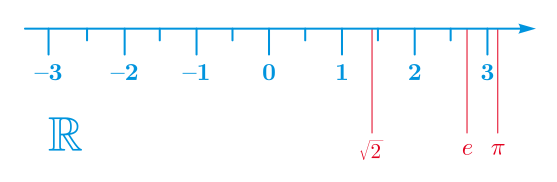
\includegraphics{./img/topologia-reales/recta-real.png}

}

\caption{La recta real}

\end{figure}

\hypertarget{intervalos-y-entornos}{%
\section{Intervalos y entornos}\label{intervalos-y-entornos}}

\leavevmode\vadjust pre{\hypertarget{def-intervalo-abierto}{}}%
\begin{definition}[Intervalo abierto]\label{def-intervalo-abierto}

Dados dos números reales tales que \(a\leq b\), se llama \emph{intervalo
abierto} de extremos \(a\) y \(b\), y se denota \((a,b)\) al conjunto de
números reales comprendidos entre \(a\) y \(b\) \[
(a,b) = \{x\in \mathbb{R}: a<x<b\}.
\]

\end{definition}

\leavevmode\vadjust pre{\hypertarget{def-intervalo-cerrado}{}}%
\begin{definition}[Intervalo cerrado]\label{def-intervalo-cerrado}

Dados dos números reales tales que \(a\leq b\), se llama \emph{intervalo
cerrado} de extremos \(a\) y \(b\), y se denota \([a,b]\) al conjunto de
números reales que son mayores o iguales que \(a\) y menores o iguales
que \(b\) \[
[a,b] = \{x\in \mathbb{R}: a\leq x\leq b\}.
\]

\end{definition}

\begin{tcolorbox}[enhanced jigsaw, left=2mm, colframe=quarto-callout-warning-color-frame, rightrule=.15mm, opacityback=0, leftrule=.75mm, colback=white, toprule=.15mm, breakable, bottomtitle=1mm, titlerule=0mm, toptitle=1mm, arc=.35mm, title=\textcolor{quarto-callout-warning-color}{\faExclamationTriangle}\hspace{0.5em}{Advertencia}, bottomrule=.15mm, opacitybacktitle=0.6, coltitle=black, colbacktitle=quarto-callout-warning-color!10!white]
Obsérvese que si \(a=b\), \((a,a)=\emptyset\) y \([a,a]=\{a\}\).
\end{tcolorbox}

Los intervalos también pueden ser abiertos por un lado y cerrados por el
otro.

\leavevmode\vadjust pre{\hypertarget{def-intervalo-semiabierto}{}}%
\begin{definition}[Intervalo semiabierto o
semicerrado]\label{def-intervalo-semiabierto}

Dados dos números reales tales que \(a<b\), se definen los
\emph{intervalos semiabiertos} o \emph{semicerrados} de extremos \(a\) y
\(b\) de la siguiente manera: \[
(a,b] = \{x\in \mathbb{R}: a< x\leq b\}\quad \mbox{y}\quad [a,b) = \{x\in \mathbb{R}: a\leq x< b\}
\]

\end{definition}

Estos intervalos están \emph{acotados} ya que \(a\) es una cota inferior
y \(b\) una cota superior, pero también existen intervalos no acotados.

\leavevmode\vadjust pre{\hypertarget{def-intervalo-abierto-no-acotado}{}}%
\begin{definition}[Intervalo abierto no
acotado]\label{def-intervalo-abierto-no-acotado}

Dado un número \(a\in \mathbb{R}\), se definen los siguientes
\emph{intervalos abiertos no acotados}: \[
(-\infty,a) = \{x\in \mathbb{R}: x<a\} \quad \mbox{y}\quad (a,\infty) = \{x\in \mathbb{R}: a< x\}
\]

\end{definition}

\leavevmode\vadjust pre{\hypertarget{def-intervalo-semiabierto-no-acotado}{}}%
\begin{definition}[Intervalo semiabierto no
acotado]\label{def-intervalo-semiabierto-no-acotado}

Dado un número \(a\in \mathbb{R}\), se definen los siguientes
\emph{intervalos semiabiertos no acotados}: \[
(-\infty,a] = \{x\in \mathbb{R}: x\leq a\} \quad \mbox{y}\quad [a,\infty) = \{x\in \mathbb{R}: a\leq x\}
\]

\end{definition}

\leavevmode\vadjust pre{\hypertarget{def-intervalos-anidados}{}}%
\begin{definition}[Intervalos anidados]\label{def-intervalos-anidados}

Se dice que una sucesión de intervalos \(I_n\), \(n\in\mathbb{N}\) es
una \emph{sucesión de intervalos anidados} si se cumple que
\(I_{n+1}\subseteq I_n\) \(\forall n\in\mathbb{N}\).

\end{definition}

\leavevmode\vadjust pre{\hypertarget{exm-sucesion-intervalos-anidados}{}}%
\begin{example}[]\label{exm-sucesion-intervalos-anidados}

La sucesión de intervalos \(I_n=[0,\frac{1}{n}]\),
\(\forall n\in\mathbb{N}\) es una sucesión de intervalos anidados, ya
que para cada \(n\in\mathbb{N}\) se cumple que \(n<n+1\) y por tanto
\(\frac{1}{n}>\frac{1}{n+1}\), de manera que
\(I_{n+1}=[0,\frac{1}{n+1}]\subseteq [0,\frac{1}{n}]=I_n\).

\end{example}

\leavevmode\vadjust pre{\hypertarget{thm-intervalos-anidados}{}}%
\begin{theorem}[Intervalos anidados]\label{thm-intervalos-anidados}

Dada una sucesión de intervalos cerrados y anidados \(I_n=[a_n,b_n]\),
\(n\in\mathbb{N}\), existe un número \(a\in\mathbb{R}\) tal que
\(a\in I_n\) \(\forall n\in\mathbb{N}\). Además, si el ínfimo de las
longitudes \(\{b_n-a_n: n\in \mathbb{N}\}\) es \(0\), entonces \(a\) es
único, es decir, \(\cap_{n=1}^\infty I_n=\{a\}\).

\end{theorem}

\begin{tcolorbox}[enhanced jigsaw, left=2mm, colframe=quarto-callout-note-color-frame, rightrule=.15mm, opacityback=0, leftrule=.75mm, colback=white, toprule=.15mm, breakable, bottomtitle=1mm, titlerule=0mm, toptitle=1mm, arc=.35mm, title=\textcolor{quarto-callout-note-color}{\faInfo}\hspace{0.5em}{Demostración}, bottomrule=.15mm, opacitybacktitle=0.6, coltitle=black, colbacktitle=quarto-callout-note-color!10!white]

\begin{proof}

Sea \(A=\{a_n: n\in\mathbb{N}\}\) y \(B=\{b_n: n\in\mathbb{N}\}\).
Puesto que los intervalos están anidados, \(A\) está acotado
superiormente por \(b_1\) ya que \(a_n\leq b_n\leq b_1\)
\(\forall n\in \mathbb{N}\), y \(B\) está acotado inferiormente por
\(a_1\) ya que \(a_1\leq a_n\leq b_n\) \(\forall n\in \mathbb{N}\). Así
pues, como \(A\) está acotado superiormente, por el axioma del supremo,
existe \(a=\sup(A)\), y como \(B\) está acotado inferiormente, existe
\(b=\inf(B)\).

Veamos ahora que \(a\leq b\). Para ello basta probar que \(a\) es cota
inferior de \(B\). Para cualquier \(n\in\mathbb{N}\) se cumple que si
\(k\geq n\) entonces \(a_k\leq b_k\leq b_n\) pues \(I_n\subseteq I_k\),
y si \(k<n\), entonces \(a_k\leq a_n\leq b_n\), pues
\(I_n\subseteq I_k\). Luego \(b_n\) es una cota superior de \(A\), y por
tanto, \(a\leq b_n\) \(\forall n\in\mathbb{N}\), de manera que \(a\) es
cota inferior de \(B\). Así pues, como \(a\) es cota superior de \(A\) e
inferior de \(B\), se tiene que \(a_n\leq a\leq b_n\)
\(\forall n\in\mathbb{N}\), de manera que
\(a\in \cap_{n=1}^\infty I_n\).

De forma similar se puede probar que \(b\in \cap_{n=1}^\infty I_n\), por
lo que \(\cap_{n=1}^\infty I_n = [a,b]\).

Finalmente, veamos que si \(\inf(\{b_n-a_n: n\in \mathbb{N}\})=0\)
entonces \(a=b\). Para ello, dado \(\varepsilon>0\), como
\(\inf(\{b_n-a_n: n\in \mathbb{N}\})=0\), existe \(k\in\mathbb{N}\) tal
que \(0\leq b_k-a_k < \varepsilon\). Como \(b\leq b_k\) y \(a\geq a_k\),
se tiene que \(0\leq b-a\leq b_k-a_k < \varepsilon\), de donde se deduce
que \(b-a=0\) y por tanto \(a=b\), así que
\(\cap_{n=1}^\infty I_n = [a,a]=\{a\}\).

\end{proof}

\end{tcolorbox}

\leavevmode\vadjust pre{\hypertarget{def-entorno}{}}%
\begin{definition}[Entorno]\label{def-entorno}

Dado un número \(a\in \mathbb{R}\), se llama \emph{entorno} de \(a\) a
cualquier intervalo abierto \((a-\varepsilon, a+\varepsilon)\) con
\(\varepsilon>0\). El número \(\varepsilon\) se conoce como \emph{radio
del entorno}.

Para cualquier \(\varepsilon>0\) el conjunto
\((a-\varepsilon, a+\varepsilon)\setminus \{a\}\) se llama \emph{entorno
reducido} de \(a\).

\end{definition}

\hypertarget{clasificaciuxf3n-de-puntos}{%
\section{Clasificación de puntos}\label{clasificaciuxf3n-de-puntos}}

Un conjunto \(A\subset \mathbb{R}\) clasifica los puntos de
\(\mathbb{R}\) en tres clases: puntos interiores, puntos exteriores y
puntos fronteras de \(A\).

\leavevmode\vadjust pre{\hypertarget{def-punto-interior}{}}%
\begin{definition}[Punto interior]\label{def-punto-interior}

Se dice que \(a\in \mathbb{R}\) es un \emph{punto interior} de un
conjunto \(A\subseteq \mathbb{R}\), si existe un entorno de \(a\)
contenido en \(A\), es decir, existe \(\varepsilon>0\) tal que
\((a-\varepsilon, a+\varepsilon) \subseteq A\).

El conjunto de los puntos interiores de \(A\) se llama \emph{interior}
de \(A\) y se denota por \(\operatorname{Int}(A)\).

\end{definition}

Aunque la definición no lo hace explícito, es evidente que si \(a\) es
un punto interior de \(A\) entonces \(a\in A\).

Intuitivamente, un punto interior de un conjunto es un punto que no está
en el borde del conjunto, es decir, que está rodeado por puntos del
conjunto, y por tanto, podemos movernos un poco hacia la izquierda o
hacia la derecha del punto sin salirnos del conjunto.

\leavevmode\vadjust pre{\hypertarget{exm-punto-interior}{}}%
\begin{example}[]\label{exm-punto-interior}

\(0.9\) es un punto interior del intervalo \((0,1)\) ya que podemos
tomar \(\varepsilon = 0.01\) tal que el entorno
\((0.9-0.01,0.9+0.01) = (0.89, 0.91)\subset (0,1)\).

Sin embargo, \(1\) no es un punto interior del intervalo \((0,1)\) ya
que por muy pequeño que tomemos \(\varepsilon>0\), \(1+\varepsilon > 1\)
y, por tanto, el entorno \((1-\varepsilon, 1+\varepsilon)\) siempre
tendrá valores mayores que 1, de manera que
\((1-\varepsilon, 1+\varepsilon)\not \subseteq (0,1)\).

\end{example}

\leavevmode\vadjust pre{\hypertarget{def-punto-exterior}{}}%
\begin{definition}[Punto exterior]\label{def-punto-exterior}

Se dice que \(a\in \mathbb{R}\) es un \emph{punto exterior} de un
conjunto \(A\subseteq \mathbb{R}\), si existe un entorno de \(a\)
contenido en el complementario de \(A\), es decir, existe
\(\varepsilon>0\) tal que
\((x-\varepsilon, x+\varepsilon) \subseteq \overline A\).

El conjunto de los puntos exteriores de \(A\) se llama \emph{exterior}
de \(A\) y se denota por \(\operatorname{Ext}(A)\).

\end{definition}

Una definición equivalente es que un punto es punto exterior de un
conjunto si es un punto interior de su complementario.

\leavevmode\vadjust pre{\hypertarget{exm-punto-exterior}{}}%
\begin{example}[]\label{exm-punto-exterior}

\(1.01\) es un punto exterior del conjunto \((-\infty, 1)\) ya que
tomando \(\varepsilon=0.001\) el entorno
\((1.01-0.001, 1.01+0.001)=(1.009, 1.011)\in \overline{(-\infty, 1)}=[1,\infty)\).

Sin embargo, \(1\) no es un punto exterior del intervalo
\((-\infty, 1)\), ya que no es un punto interior del intervalo
\(\overline{(-\infty, 1)}=[1,\infty)\), ya que \(1-\varepsilon < 1\)
\(\forall \varepsilon>0\), y, por tanto, el entorno
\((1-\varepsilon, 1+\varepsilon)\) siempre tendrá valores menores que 1,
de manera que
\((1-\varepsilon, 1+\varepsilon)\not \subseteq [1,\infty)\).

\end{example}

\begin{tcolorbox}[enhanced jigsaw, left=2mm, colframe=quarto-callout-warning-color-frame, rightrule=.15mm, opacityback=0, leftrule=.75mm, colback=white, toprule=.15mm, breakable, bottomtitle=1mm, titlerule=0mm, toptitle=1mm, arc=.35mm, title=\textcolor{quarto-callout-warning-color}{\faExclamationTriangle}\hspace{0.5em}{Advertencia}, bottomrule=.15mm, opacitybacktitle=0.6, coltitle=black, colbacktitle=quarto-callout-warning-color!10!white]
El que un punto no sea punto interior de un conjunto no significa que
sea un punto exterior. Por ejemplo, \(1\) no es un punto interior del
intervalo \((0,1)\), y tampoco de su complementario
\(\overline{(0,1)}=(-\infty, 0]\cup[ñ1,\infty)\).
\end{tcolorbox}

\leavevmode\vadjust pre{\hypertarget{def-punto-frontera}{}}%
\begin{definition}[Punto frontera]\label{def-punto-frontera}

Se dice que \(a\in \mathbb{R}\) es un \emph{punto frontera} de un
conjunto \(A\subseteq \mathbb{R}\), si cualquier entorno de \(a\)
contiene puntos de \(A\) y de su complementario.

El conjunto de los puntos frontera de \(A\) se llama \emph{frontera} de
\(A\) y se denota por \(\operatorname{Fr}(A)\).

\end{definition}

Una definición equivalente es que un punto es un punto frontera de un
conjunto si no es un punto interior ni exterior del conjunto.

\leavevmode\vadjust pre{\hypertarget{exm-punto-frontera}{}}%
\begin{example}[]\label{exm-punto-frontera}

El punto \(1\) es un punto frontera del intervalo \([1,\infty)\) ya que
no es un punto interior de \([1,\infty)\) ni de su complementario
\((-\infty,1)\).

\end{example}

\leavevmode\vadjust pre{\hypertarget{prp-interior-intervalo-abierto}{}}%
\begin{proposition}[]\label{prp-interior-intervalo-abierto}

Todos los puntos de un intervalo abierto son puntos interiores suyos, es
decir, dado un intervalo abierto \((a,b)\subseteq \mathbb{R}\), se
cumple que \(\operatorname{Int}((a,b)) = (a,b)\).

\end{proposition}

\begin{tcolorbox}[enhanced jigsaw, left=2mm, colframe=quarto-callout-note-color-frame, rightrule=.15mm, opacityback=0, leftrule=.75mm, colback=white, toprule=.15mm, breakable, bottomtitle=1mm, titlerule=0mm, toptitle=1mm, arc=.35mm, title=\textcolor{quarto-callout-note-color}{\faInfo}\hspace{0.5em}{Demostración}, bottomrule=.15mm, opacitybacktitle=0.6, coltitle=black, colbacktitle=quarto-callout-note-color!10!white]

\begin{proof}

Tomemos cualquier punto \(x\in (a,b)\), entonces se puede tomar
\(\varepsilon = \frac{\min\{|x-a|,|x-b\}}{2}\) de manera que el entorno
\((x-\varepsilon, x+\varepsilon)\subseteq (a,b)\).

\end{proof}

\end{tcolorbox}

\leavevmode\vadjust pre{\hypertarget{prp-interior-intervalo-cerrado}{}}%
\begin{proposition}[]\label{prp-interior-intervalo-cerrado}

Todos los puntos de un intervalo cerrado, excepto sus extremos, son
puntos interiores suyos, es decir, dado un intervalo cerrado
\([a,b]\subseteq \mathbb{R}\), se cumple que
\(\operatorname{Int}([a,b]) = (a,b)\).

\end{proposition}

\begin{tcolorbox}[enhanced jigsaw, left=2mm, colframe=quarto-callout-note-color-frame, rightrule=.15mm, opacityback=0, leftrule=.75mm, colback=white, toprule=.15mm, breakable, bottomtitle=1mm, titlerule=0mm, toptitle=1mm, arc=.35mm, title=\textcolor{quarto-callout-note-color}{\faInfo}\hspace{0.5em}{Demostración}, bottomrule=.15mm, opacitybacktitle=0.6, coltitle=black, colbacktitle=quarto-callout-note-color!10!white]

\begin{proof}

Par ver que \(a\) no es un punto interior de \([a,b]\), basta con ver
que \(a-\varepsilon < a\) para cualquier \(\varepsilon>0\), por lo que
el intervalo \((a-\varepsilon,a+\varepsilon)\) irremediablemente
contendrá puntos menores que \(a\) y, por tanto,
\((a-\varepsilon,a+\varepsilon)\not \subseteq [a,b]\).

Un razonamiento análogo se puede utilizar para demostrar que \(b\)
tampoco es un punto interior de \([a,b]\).

\end{proof}

\end{tcolorbox}

A partir de estas proposiciones, es fácil ver que que para cualquier
intervalo abierto \((a,b)\), \(\operatorname{Int}((a,b)) = (a,b)\),
\(\operatorname{Ext}((a,b)) = (-\infty,a)\cup (b,\infty)\) y
\(\operatorname{Fr}((a,b)) = \{a, b\}\). Y para cualquier intervalo
cerrado \([a,b]\), \(\operatorname{Int}([a,b]) = (a,b)\),
\(\operatorname{Ext}([a,b]) = (-\infty,a)\cup (b,\infty)\) y
\(\operatorname{Fr}([a,b]) = \{a, b\}\).

\leavevmode\vadjust pre{\hypertarget{prp-clasifiacion-puntos}{}}%
\begin{proposition}[]\label{prp-clasifiacion-puntos}

Dado un conjunto \(A\subset \mathbb{R}\), los conjuntos
\(\operatorname{Int}(A)\), \(\operatorname{Ext}(A)\) y
\(\operatorname{Fr}(A)\) forman una partición de \(\mathbb{R}\), es
decir,

\begin{enumerate}
\def\labelenumi{\alph{enumi}.}
\tightlist
\item
  \(\operatorname{Int}(A)\), \(\operatorname{Ext}(A)\) y
  \(\operatorname{Fr}(A)\) son disjuntos entre sí.
\item
  \(\operatorname{Int}(A)\cup \operatorname{Ext}(A)\cup \operatorname{Fr}(A) = \mathbb{R}\).
\end{enumerate}

\end{proposition}

\begin{tcolorbox}[enhanced jigsaw, left=2mm, colframe=quarto-callout-note-color-frame, rightrule=.15mm, opacityback=0, leftrule=.75mm, colback=white, toprule=.15mm, breakable, bottomtitle=1mm, titlerule=0mm, toptitle=1mm, arc=.35mm, title=\textcolor{quarto-callout-note-color}{\faInfo}\hspace{0.5em}{Demostración}, bottomrule=.15mm, opacitybacktitle=0.6, coltitle=black, colbacktitle=quarto-callout-note-color!10!white]

\begin{proof}

Se deja como ejercicio.

\end{proof}

\end{tcolorbox}

A continuación se definen otros tipos de puntos que son útiles para
definir conceptos que se verán más adelante como el de \emph{límite}.

\leavevmode\vadjust pre{\hypertarget{def-punto-adherente}{}}%
\begin{definition}[Punto adherente]\label{def-punto-adherente}

Se dice que \(a\in \mathbb{R}\) es un \emph{punto adherente} de un
conjunto \(A\subseteq \mathbb{R}\), si cualquier entorno de \(a\)
contiene puntos de \(A\).

El conjunto de los puntos adherentes de \(A\) se llama \emph{adherencia}
de \(A\) y se denota por \(\operatorname{Adh}(A)\).

\end{definition}

Resulta obvio que cualquier punto interior y frontera de un conjunto es
también adherente, y que cualquier punto exterior no es adherente.
Resulta evidente también que cualquier punto de un conjunto es un punto
adherente, de manera que para cualquier conjunto \(A\) se tiene
\(A\subseteq\operatorname{Adh}(A)\).

\leavevmode\vadjust pre{\hypertarget{def-punto-acumulacion}{}}%
\begin{definition}[Punto de acumulacion]\label{def-punto-acumulacion}

Se dice que \(a\in \mathbb{R}\) es un \emph{punto de acumulación} de un
conjunto \(A\subseteq \mathbb{R}\), si cualquier entorno reducido de
\(a\) contiene puntos de \(A\).

El conjunto de los puntos de acumulación de \(A\) se llama
\emph{conjunto derivado} de \(A\) y se denota por
\(\operatorname{Ac}(A)\).

\end{definition}

\begin{tcolorbox}[enhanced jigsaw, left=2mm, colframe=quarto-callout-warning-color-frame, rightrule=.15mm, opacityback=0, leftrule=.75mm, colback=white, toprule=.15mm, breakable, bottomtitle=1mm, titlerule=0mm, toptitle=1mm, arc=.35mm, title=\textcolor{quarto-callout-warning-color}{\faExclamationTriangle}\hspace{0.5em}{Advertencia}, bottomrule=.15mm, opacitybacktitle=0.6, coltitle=black, colbacktitle=quarto-callout-warning-color!10!white]
Resulta obvio de la definición que cualquier punto de acumulación es
también un punto de adherencia, es decir,
\(\operatorname{Ac}(A)\subseteq \operatorname{Adh}(A)\) para cualquier
conjunto \(A\subset \mathbb{R}\). Sin embargo no todo punto de
adherencia es un punto de acumulación.
\end{tcolorbox}

Es posible que un conjunto tenga puntos de acumulación que pertenezcan
al conjunto y otros que no.

\leavevmode\vadjust pre{\hypertarget{exm-puntos-adherentes-acumulacion}{}}%
\begin{example}[]\label{exm-puntos-adherentes-acumulacion}

Dado el conjunto \(A=(0,1) \cup \{2\}\), se tiene que \(2\) es un punto
de adherencia de \(A\), pues para cualquier \(\varepsilon>0\) el entorno
\((2-\varepsilon,2+\varepsilon)\) contiene al propio \(2\) que es un
punto de \(A\). Sin embargo, \(2\) no es un punto de acumulación, porque
para \(\varepsilon=0.5\), por ejemplo, el entorno reducido
\((2-\varepsilon,2+\varepsilon)\setminus\{2\}=(1.5,2)\cup(2,2.5)\) no
contiene puntos de \(A\).

En cambio el punto \(0.5\) es tanto un punto de adherencia como un punto
de acumulación de \(A\) porque para cualquier \(\varepsilon>0\) el
entorno reducido \((0.5-\varepsilon,0.5+\varepsilon)\setminus \{0.5\}\)
siempre contiene puntos de \(A\). De hecho, para cualquier \(x\in(a,b)\)
y para cualquier \(\varepsilon>0\), el intervalo
\((x-\varepsilon,x+\varepsilon)\setminus \{x\}\) contiene puntos de
\(A\), y lo mismo ocurre para \(a\) y \(b\) al ser puntos frontera, de
manera que \(\operatorname{Ac}(A)=[0,1]\), mientras que
\(\operatorname{Adh}(A)=[0,1]\cup\{2\}\).

\end{example}

Intuitivamente, un punto de acumulación de un conjunto \(A\) es un punto
para el que podemos encontrar puntos de \(A\), distintos de él mismo,
tan próximos a él como queramos. Un punto de acumulación se diferencia
de un punto de adherencia en que siempre está rodeado por puntos de
\(A\), mientras que un punto de adherencia puede estar aislado de los
demás puntos de \(A\).

\leavevmode\vadjust pre{\hypertarget{def-punto-aislado}{}}%
\begin{definition}[Punto aislado]\label{def-punto-aislado}

Se dice que \(a\in \mathbb{R}\) es un \emph{punto de aislado} de un
conjunto \(A\subseteq \mathbb{R}\), si es un punto adherente de \(A\),
pero no de acumulación.

\end{definition}

\leavevmode\vadjust pre{\hypertarget{prp-punto-adherente-acumulacion}{}}%
\begin{proposition}[]\label{prp-punto-adherente-acumulacion}

Para cualquier intervalo abierto \((a,b)\) se tiene que
\(\operatorname{Adh}((a,b))=\operatorname{Ac}((a,b))=[a,b]\).

\end{proposition}

\begin{tcolorbox}[enhanced jigsaw, left=2mm, colframe=quarto-callout-note-color-frame, rightrule=.15mm, opacityback=0, leftrule=.75mm, colback=white, toprule=.15mm, breakable, bottomtitle=1mm, titlerule=0mm, toptitle=1mm, arc=.35mm, title=\textcolor{quarto-callout-note-color}{\faInfo}\hspace{0.5em}{Demostración}, bottomrule=.15mm, opacitybacktitle=0.6, coltitle=black, colbacktitle=quarto-callout-note-color!10!white]

\begin{proof}

Todos los puntos de \((a,b)\) son interiores y, por tanto, para
cualquier \(x\in (a,b)\), existe un \(\varepsilon>0\) tal que
\((x-\varepsilon,x+\varepsilon)\subseteq (a,b)\). Si ahora tomamos
cualquier otro \(\varepsilon'>0\), se tiene que
\((x-\varepsilon',x+\varepsilon')\setminus \{x\}\cap(x-\varepsilon,x+\varepsilon)\neq \emptyset\),
pero como \((x-\varepsilon,x+\varepsilon)\subseteq (a,b)\), se concluye
que
\((x-\varepsilon',x+\varepsilon')\setminus \{x\}\cap (a,b)\neq \emptyset\),
por lo que \(x\) es un punto de acumulación de \((a,b)\). Por otro lado,
como \(a\) y \(b\) son puntos frontera, también se tiene que para
cualquier \(\varepsilon>0\),
\((a-\varepsilon,a+\varepsilon)\cap (a,b)\neq \emptyset\) y
\((b-\varepsilon,b+\varepsilon)\cap (a,b)\neq \emptyset\) de manera que
\([a,b]\subseteq \operatorname{Ac}((a,b))\subseteq \operatorname{Adh}((a,b))\).
Sea ahora cualquier \(x>b\), y tomemos \(\varepsilon=\frac{|x-b|}{2}\),
entonces \((x-\varepsilon, x+\varepsilon)\cap (a,b)=\emptyset\), de
manera que \(x\) no es un punto de adherencia de \((a,b)\). Del mismo
modo se puede probar que si \(x<a\), entonces \(x\) tampoco es un punto
de adherencia de \((a,b)\), por lo que
\(\operatorname{Adh}((a,b))=[a,b]\) y como
\(\operatorname{Ac}((a,b))\subseteq \operatorname{Adh}((a,b))\), también
se concluye que \(\operatorname{Ac}((a,b))=[a,b]\).

\end{proof}

\end{tcolorbox}

\leavevmode\vadjust pre{\hypertarget{prp-adherencia-conjunto-mas-acumulacion}{}}%
\begin{proposition}[]\label{prp-adherencia-conjunto-mas-acumulacion}

Para cualquier conjunto \(A\subseteq \mathbb{R}\), se tiene que
\(\operatorname{Adh}(A)=A\cup \operatorname{Ac}(A)\).

\end{proposition}

\begin{tcolorbox}[enhanced jigsaw, left=2mm, colframe=quarto-callout-note-color-frame, rightrule=.15mm, opacityback=0, leftrule=.75mm, colback=white, toprule=.15mm, breakable, bottomtitle=1mm, titlerule=0mm, toptitle=1mm, arc=.35mm, title=\textcolor{quarto-callout-note-color}{\faInfo}\hspace{0.5em}{Demostración}, bottomrule=.15mm, opacitybacktitle=0.6, coltitle=black, colbacktitle=quarto-callout-note-color!10!white]

\begin{proof}

Ya se ha visto que \(A\subseteq \operatorname{Adh}(A)\) y también
\(\operatorname{Ac}(A)\subseteq \operatorname{Adh}(A)\), por lo que
\(A\cup \operatorname{Ac}(A)\subseteq \operatorname{Adh}(A)\).

Veamos ahora que
\(\operatorname{Adh}(A)\subseteq A\cup \operatorname{Ac}(A)\). Sea \(x\)
un punto de adherencia de \(A\). Si \(x\in A\) es obvio que
\(x\in A\cup \operatorname{Ac}(A)\), y si \(x\not\in A\), entonces
\(x\in \operatorname{Ac}(A)\), ya que, por ser \(x\) punto de adherencia
de \(A\), para cualquier \(\varepsilon>0\),
\((x-\varepsilon,x+\varepsilon)\cap A\neq \emptyset\), pero como además
\(x\not\in A\), también se cumple que el entorno reducido
\((x-\varepsilon,x+\varepsilon)\setminus\{x\}\) contiene puntos de
\(A\). Así pues, \(x\in A\cup \operatorname{Ac}(A)\), y por tanto
\(\operatorname{Adh}(A)\subseteq A\cup \operatorname{Ac}(A)\).

\end{proof}

\end{tcolorbox}

\hypertarget{conjuntos-abiertos-y-cerrados}{%
\section{Conjuntos abiertos y
cerrados}\label{conjuntos-abiertos-y-cerrados}}

A continuación se generaliza la característica que diferencia los
intervalos abiertos y cerrados, a cualquier conjunto.

\leavevmode\vadjust pre{\hypertarget{def-conjunto-abierto}{}}%
\begin{definition}[Conjunto abierto]\label{def-conjunto-abierto}

Se dice que un conjunto \(A\subset \mathbb{R}\) es \emph{abierto} cuando
para cada \(a\in A\) existe un entorno de \(a\) contenido en \(A\), es
decir, existe \(\varepsilon>0\) tal que
\((a-\varepsilon, a+\varepsilon)\subset A\).

\end{definition}

\begin{tcolorbox}[enhanced jigsaw, left=2mm, colframe=quarto-callout-important-color-frame, rightrule=.15mm, opacityback=0, leftrule=.75mm, colback=white, toprule=.15mm, breakable, bottomtitle=1mm, titlerule=0mm, toptitle=1mm, arc=.35mm, title=\textcolor{quarto-callout-important-color}{\faExclamation}\hspace{0.5em}{Importante}, bottomrule=.15mm, opacitybacktitle=0.6, coltitle=black, colbacktitle=quarto-callout-important-color!10!white]
Obsérvese que un conjunto es abierto si todos sus puntos son interiores.
\end{tcolorbox}

\leavevmode\vadjust pre{\hypertarget{exm-intervalo-abierto-conjunto-abierto}{}}%
\begin{example}[]\label{exm-intervalo-abierto-conjunto-abierto}

Cualquier intervalo abierto \((a,b)\) es un conjunto abierto, ya que
según se vio en la Proposición~\ref{prp-interior-intervalo-abierto}
\(\operatorname{Int}((a,b)) = (a,b)\). Por otro lado, un intervalo
cerrado \([a,b]\) no es un conjunto abierto pues cualquier entorno de
\(a\) o \(b\) no está contenido en \([a,b]\).

\end{example}

Una colección de conjuntos abiertos se llama \emph{topología} y
cualquier propiedad que pueda definirse en términos de conjuntos
abiertos se llama \emph{propiedad topológica}.

\leavevmode\vadjust pre{\hypertarget{def-conjunto-cerrado}{}}%
\begin{definition}[Conjunto cerrado]\label{def-conjunto-cerrado}

Se dice que un conjunto \(A\subset \mathbb{R}\) es \emph{cerrado} cuando
su complementario \(\overline A =\mathbb{R}\setminus A\) es abierto.

\end{definition}

\leavevmode\vadjust pre{\hypertarget{exm-intervalo-cerrado-conjunto-cerrado}{}}%
\begin{example}[]\label{exm-intervalo-cerrado-conjunto-cerrado}

Todo intervalo cerrado \([a,b]\) es cerrado, pues su complementario
\((-\infty,a)\cup (b,\infty)\) es abierto.

\end{example}

\begin{tcolorbox}[enhanced jigsaw, left=2mm, colframe=quarto-callout-warning-color-frame, rightrule=.15mm, opacityback=0, leftrule=.75mm, colback=white, toprule=.15mm, breakable, bottomtitle=1mm, titlerule=0mm, toptitle=1mm, arc=.35mm, title=\textcolor{quarto-callout-warning-color}{\faExclamationTriangle}\hspace{0.5em}{Advertencia}, bottomrule=.15mm, opacitybacktitle=0.6, coltitle=black, colbacktitle=quarto-callout-warning-color!10!white]
Un subconjunto puede ser abierto y cerrado a la vez, como por ejemplo
\(\mathbb{R}\) y \(\emptyset\). \(\mathbb{R}\) es abierto ya que todos
sus puntos son interiores, y por tanto
\(\overline{\mathbb{R}}=\emptyset\) es cerrado. Pero, también
\(\emptyset\) es abierto, ya que para que un conjunto no sea abierto, al
menos uno de sus puntos no debe ser interior, y en consecuencia
\(\overline{\emptyset}=\mathbb{R}\) es también cerrado.

Un subconjunto también puede no ser abierto ni cerrado, como por ejemplo
\((a,b]\), ya que \(b\) no es un punto interior de \((a,b]\), y \(a\) no
es un punto interior de \(\overline{(a,b]}=(-\infty,a]\cup (b,\infty)\).
Por tanto, no abierto no implica cerrado y no cerrado no implica
abierto.
\end{tcolorbox}

\leavevmode\vadjust pre{\hypertarget{prp-union-interseccion-conjuntos-abiertos-cerrados}{}}%
\begin{proposition}[]\label{prp-union-interseccion-conjuntos-abiertos-cerrados}

Se cumplen las siguientes propiedades:

\begin{enumerate}
\def\labelenumi{\arabic{enumi}.}
\tightlist
\item
  La unión de una colección de conjuntos abiertos es un conjunto
  abierto.
\item
  La intersección de una colección finita de conjuntos abiertos es un
  conjunto abierto.
\item
  La intersección de una colección de conjuntos cerrados es cerrada.
\item
  La unión de una colección finita de conjuntos cerrados es un conjunto
  cerrado.
\end{enumerate}

\end{proposition}

\begin{tcolorbox}[enhanced jigsaw, left=2mm, colframe=quarto-callout-note-color-frame, rightrule=.15mm, opacityback=0, leftrule=.75mm, colback=white, toprule=.15mm, breakable, bottomtitle=1mm, titlerule=0mm, toptitle=1mm, arc=.35mm, title=\textcolor{quarto-callout-note-color}{\faInfo}\hspace{0.5em}{Demostración}, bottomrule=.15mm, opacitybacktitle=0.6, coltitle=black, colbacktitle=quarto-callout-note-color!10!white]

\begin{proof}

Se deja como ejercicio.

\end{proof}

\end{tcolorbox}

\begin{tcolorbox}[enhanced jigsaw, left=2mm, colframe=quarto-callout-warning-color-frame, rightrule=.15mm, opacityback=0, leftrule=.75mm, colback=white, toprule=.15mm, breakable, bottomtitle=1mm, titlerule=0mm, toptitle=1mm, arc=.35mm, title=\textcolor{quarto-callout-warning-color}{\faExclamationTriangle}\hspace{0.5em}{Advertencia}, bottomrule=.15mm, opacitybacktitle=0.6, coltitle=black, colbacktitle=quarto-callout-warning-color!10!white]
La intersección de una colección infinita de conjuntos abiertos puede no
ser un conjunto abierto, como por ejemplo la colección de conjuntos
\(I_n=(0,1+\frac{1}{n})\), \(n\in\mathbb{N}\), ya que
\(\cap_{n=1}^\infty I_n=(0,1]\).

Y la unión de una colección infinita de conjuntos cerrados puede no ser
cerrada, como por ejemplo la colección de conjuntos
\(J_n=[\frac{1}{n},1]\), \(n\in\mathbb{N}\), ya que
\(\cup_{n=1}^\infty J_n=(0,1]\).
\end{tcolorbox}

\leavevmode\vadjust pre{\hypertarget{thm-existencia-maximo-minimo}{}}%
\begin{theorem}[Existencia del máximo y
mínimo]\label{thm-existencia-maximo-minimo}

Cualquier conjunto no-vacío, cerrado y acotado superiormente tiene un
máximo, y cualquier conjunto no-vacío, cerrado y acotado inferiormente
tiene un mínimo.

\end{theorem}

\begin{tcolorbox}[enhanced jigsaw, left=2mm, colframe=quarto-callout-note-color-frame, rightrule=.15mm, opacityback=0, leftrule=.75mm, colback=white, toprule=.15mm, breakable, bottomtitle=1mm, titlerule=0mm, toptitle=1mm, arc=.35mm, title=\textcolor{quarto-callout-note-color}{\faInfo}\hspace{0.5em}{Demostración}, bottomrule=.15mm, opacitybacktitle=0.6, coltitle=black, colbacktitle=quarto-callout-note-color!10!white]

\begin{proof}

Sea \(A\) un conjunto no vacío, cerrado y acotado superiormente. Como
\(A\) está acotado superiormente, por el axioma del supremo, existe
\(s=\sup(A)\). Probaremos que \(s\in A\) por reducción al absurdo.
Supongamos que \(s\not\in A\), entonces \(s\in\overline{A}\), y como
\(\overline{A}\) es abierto al ser \(A\) cerrado, existe un
\(\varepsilon>0\) tal que
\((s-\varepsilon, s+\varepsilon)\subseteq \overline{A}\). Como ningún
elemento de \(A\) puede ser mayor que \(s\) y
\((s-\varepsilon, s+\varepsilon)\not\subseteq A\), se tiene que
\(s-\varepsilon\) es también una cota superior de \(A\), pero
\(s-\varepsilon <s\), lo que contradice que \(s\) sea el supremo de
\(A\). Así, pues \(s\in A\), y por tanto es el máximo de \(A\).

De manera análoga se prueba que si \(A\) un conjunto no vacío, cerrado y
acotado inferiormente, \(A\) tiene mínimo.

\end{proof}

\end{tcolorbox}

\leavevmode\vadjust pre{\hypertarget{thm-bolzano-weierstrass}{}}%
\begin{theorem}[Bolzano-Weierstrass]\label{thm-bolzano-weierstrass}

Todo subconjunto infinito de \(\mathbb{R}\) acotado tiene al menos un
punto de acumulación.

\end{theorem}

\begin{tcolorbox}[enhanced jigsaw, left=2mm, colframe=quarto-callout-note-color-frame, rightrule=.15mm, opacityback=0, leftrule=.75mm, colback=white, toprule=.15mm, breakable, bottomtitle=1mm, titlerule=0mm, toptitle=1mm, arc=.35mm, title=\textcolor{quarto-callout-note-color}{\faInfo}\hspace{0.5em}{Demostración}, bottomrule=.15mm, opacitybacktitle=0.6, coltitle=black, colbacktitle=quarto-callout-note-color!10!white]

\begin{proof}

Para demostrar el teorema construiremos una sucesión de intervalos
cerrados y anidados y aplicaremos el
Teorema~\ref{thm-intervalos-anidados}.

Sea \(A\subset \mathbb{R}\) un subconjunto infinito y acotado. Como
\(A\) está acotado, existe un intervalo cerrado tal que
\(A\subset I_1=[a_1,b_1]\). Si \(I_1\) se divide en dos intervalos
\([a_1, \frac{a_1+b_1}{2}]\) y \([\frac{a_1+b_1}{2}, b_1]\), al menos
uno de estos intervalos tendrá infinitos puntos de \(A\), ya que de lo
contrario \(A\) sería finito. Sea \(I_2=[a_2,b_2]\) cualquiera de los
dos intervalos que tenga infinitos puntos de \(A\). Si \(I_2\) se divide
en dos intervalos \([a_2, \frac{a_2+b_2}{2}]\) y
\([\frac{a_2+b_2}{2}, b_2]\), al menos uno de estos intervalos tendrá
infinitos puntos de \(A\), ya que de lo contrario \(A\) sería finito.
Sea \(I_3=[a_3,b_3]\) cualquiera de los dos intervalos que tenga
infinitos puntos de \(A\). Siguiendo la misma lógica, se puede construir
una sucesión de intervalos anidados
\(I_1\supset I_2\supset I_3 \supset \cdots\), con tamaños
\(\frac{b_1-a_1}{2^{n-1}}\). Como
\(\inf\{\frac{b_1-a_1}{2^{n-1}}: n\in\mathbb{N}\} =0\), aplicando el
Teorema~\ref{thm-intervalos-anidados}, existe un único
\(a\in\mathbb{R}\) tal que \(\cap_{n=1}^\infty I_n=\{a\}\).

Veremos ahora que \(a\) es un punto de acumulación de \(A\). Para
cualquier \(\varepsilon>0\), considérese el entorno reducido de \(a\)
\((a-\varepsilon, a+\varepsilon)\setminus\{a\}\). Como
\(\inf\{\frac{b_1-a_1}{2^{n-1}}: n\in\mathbb{N}\} =0\), existe
\(m\in\mathbb{N}\) tal que \(\frac{b_1-a_1}{2^{m-1}}<\varepsilon\), y
por tanto \(I_m\subset (a-\varepsilon, a+\varepsilon)\), y como \(I_m\)
contiene infinitos puntos de \(A\), el entorno reducido \(a\) también
contiene puntos de \(A\), por lo que \(a\) es un punto de acumulación de
\(A\).

\end{proof}

\end{tcolorbox}

\leavevmode\vadjust pre{\hypertarget{thm-conjunto-cerrado-puntos-acumulacion}{}}%
\begin{theorem}[]\label{thm-conjunto-cerrado-puntos-acumulacion}

Cualquier subconjunto de \(\mathbb{R}\) es cerrado si y sólo si contiene
a todos sus puntos de acumulación.

\end{theorem}

\begin{tcolorbox}[enhanced jigsaw, left=2mm, colframe=quarto-callout-note-color-frame, rightrule=.15mm, opacityback=0, leftrule=.75mm, colback=white, toprule=.15mm, breakable, bottomtitle=1mm, titlerule=0mm, toptitle=1mm, arc=.35mm, title=\textcolor{quarto-callout-note-color}{\faInfo}\hspace{0.5em}{Demostración}, bottomrule=.15mm, opacitybacktitle=0.6, coltitle=black, colbacktitle=quarto-callout-note-color!10!white]

\begin{proof}

Sea \(A\subset \mathbb{R}\) un conjunto cerrado y sea \(a\in\mathbb{R}\)
un punto de acumulación de \(A\). Veamos por reducción al absurdo que
\(a\in A\).

Supongamos que \(a\not\in A\), entonces \(a\in \overline A\). Como \(A\)
es cerrado, \(\overline A\) es abierto y existe un \(\varepsilon>0\) tal
que el entorno \((a-\varepsilon, a+\varepsilon)\subset \overline A\),
pero entonces \((a-\varepsilon, a+\varepsilon)\cap A=\emptyset\), lo que
contradice que \(a\) sea punto de acumulación de \(A\).

Veremos ahora el otro sentido de la implicación. Sea \(A\) un conjunto
que contiene todos sus puntos de acumulación. Sea \(x\in \overline A\),
entonces \(x\not\in A\) y por tanto no es un punto de acumulación de
\(A\) y existe un \(\varepsilon>0\) tal que el entorno propio de \(x\)
\((x-\varepsilon, x+\varepsilon)\setminus\{x\}\cap A =\emptyset\). Como
\((x-\varepsilon, x+\varepsilon)\setminus\{x\}\subset \overline A\) y
\(x\in\overline{A}\) se concluye que
\((x-\varepsilon,x+\varepsilon)\subset \overline A\), de manera que
\(\overline{A}\) es abierto y \(A\) es cerrado.

\end{proof}

\end{tcolorbox}

\bookmarksetup{startatroot}

\hypertarget{sucesiones-de-nuxfameros-reales}{%
\chapter{Sucesiones de números
reales}\label{sucesiones-de-nuxfameros-reales}}

Las sucesiones de números reales son claves para comprender el concepto
de límite que es fundamental en el Análisis Matemático. En este capítulo
se presenta el concepto de sucesión de números reales, el concepto de
límite y algunos resultados importantes sobre la convergencia de
sucesiones.

\hypertarget{concepto-de-sucesiuxf3n}{%
\section{Concepto de sucesión}\label{concepto-de-sucesiuxf3n}}

\leavevmode\vadjust pre{\hypertarget{def-sucesion}{}}%
\begin{definition}[Sucesión de números reales]\label{def-sucesion}

Una \emph{sucesión de números reales} es una aplicación
\(x:\mathbb{N}\to \mathbb{R}\) que asigna a cada número natural un
número real, conocido como \emph{término de la sucesión}.

\end{definition}

Es habitual referirse a una sucesión con la notación
\((x_n)_{n=1}^\infty\), donde \(x_n=x(n)\) con \(n\in\mathbb{N}\), o
simplemente con \(x_n\).

\leavevmode\vadjust pre{\hypertarget{exm-sucesion1}{}}%
\begin{example}[]\label{exm-sucesion1}

La sucesión \(\left(\frac{1}{n}\right)_{n=1}^\infty\) está formada por
los términos \(\frac{1}{1}, \frac{1}{2}, \frac{1}{3}, \ldots\).

\end{example}

\begin{tcolorbox}[enhanced jigsaw, left=2mm, colframe=quarto-callout-caution-color-frame, rightrule=.15mm, opacityback=0, leftrule=.75mm, colback=white, toprule=.15mm, breakable, bottomtitle=1mm, titlerule=0mm, toptitle=1mm, arc=.35mm, title=\textcolor{quarto-callout-caution-color}{\faFire}\hspace{0.5em}{Precaución}, bottomrule=.15mm, opacitybacktitle=0.6, coltitle=black, colbacktitle=quarto-callout-caution-color!10!white]
No hay que confundir los términos de una sucesión
\((x_n)_{n=1}^\infty\), que tienen orden, con el conjunto de los valores
de la sucesión \(\{x_n:n\in\mathbb{N}\}\) que no tiene orden.
\end{tcolorbox}

\leavevmode\vadjust pre{\hypertarget{exm-sucesion2}{}}%
\begin{example}[]\label{exm-sucesion2}

La sucesión \(\left((-1)^n\right)_{n=1}^\infty\) está formada por los
términos \(-1,1,-1,1,\ldots\), mientras que
\(\{x_n:n\in\mathbb{N}\}=\{-1,1\}\).

\end{example}

Las operaciones aritméticas de los números reales se pueden extrapolar a
las sucesiones aplicándolas término a término.

\leavevmode\vadjust pre{\hypertarget{def-operaciones-sucesiones}{}}%
\begin{definition}[Operaciones con
sucesiones]\label{def-operaciones-sucesiones}

Dadas dos sucesiones de números reales \((x_n)_{n=1}^\infty\) e
\((y_n)_{n=1}^\infty\), se definen las siguientes operaciones:

\begin{itemize}
\item
  \emph{Suma:}
  \((x_n)_{n=1}^\infty + (y_n)_{n=1}^\infty = (x_n+y_n)_{n=1}^\infty\).
\item
  \emph{Diferencia:}
  \((x_n)_{n=1}^\infty - (y_n)_{n=1}^\infty = (x_n-y_n)_{n=1}^\infty\).
\item
  \emph{Producto:}
  \((x_n)_{n=1}^\infty (y_n)_{n=1}^\infty = (x_ny_n)_{n=1}^\infty\).
\item
  \emph{División:}
  \(\dfrac{(x_n)_{n=1}^\infty}{(y_n)_{n=1}^\infty} = \left(\dfrac{x_n}{y_n}\right)_{n=1}^\infty\),
  siempre y cuando \(y_n\neq 0\) \(\forall n\in\mathbb{N}\).
\item
  \emph{Producto por escalar:}
  \(c(x_n)_{n=1}^\infty = (cx_n)_{n=1}^\infty\).
\end{itemize}

\end{definition}

\leavevmode\vadjust pre{\hypertarget{exm-operaciones-sucesiones}{}}%
\begin{example}[]\label{exm-operaciones-sucesiones}

Dadas las sucesiones \((n)_{n=1}^\infty\) y \(((-1)^n)_{n=1}^\infty\) se
tiene:

\begin{align*}
(n)_{n=1}^\infty + ((-1)^n)_{n=1}^\infty &= (n + (-1)^n)_{n=1}^\infty = (0, 3, 2, 5, 4, \ldots)\\
(n)_{n=1}^\infty ((-1)^n)_{n=1}^\infty &= (n (-1)^n)_{n=1}^\infty = (-1, 2, -3, 4, -5, \ldots)
\end{align*}

\end{example}

\hypertarget{luxedmite-de-una-sucesiuxf3n}{%
\section{Límite de una sucesión}\label{luxedmite-de-una-sucesiuxf3n}}

\leavevmode\vadjust pre{\hypertarget{def-limite-sucesion}{}}%
\begin{definition}[Límite de una sucesión]\label{def-limite-sucesion}

Dada una sucesión \((x_n)_{n=1}^\infty\), se dice que un número
\(x\in\mathbb{R}\) es el \emph{límite de la sucesión}, si para cada
\(\varepsilon>0\) existe un \(k\in\mathbb{N}\) a partir del cuál todos
los términos de la sucesión caen en el entorno
\((x-\varepsilon, x+\varepsilon)\), es decir, \(|x_n-x|<\varepsilon\)
\(\forall n\geq k\).

Si \(x\) es el límite de la sucesión, se dice que la suceción
\emph{converge} a \(x\), y se denota \(\lim_{n\to\infty}x_n = x\).

\end{definition}

Si una sucesión tiene límite se dice que es \emph{convergente}, y en
caso contrario se dice que es \emph{divergente}.

\leavevmode\vadjust pre{\hypertarget{exm-limite-sucesion}{}}%
\begin{example}[]\label{exm-limite-sucesion}

La sucesión \((\frac{1}{n})_{n=1}^\infty\) es convergente y
\(\lim_{n\to\infty}\frac{1}{n} = 0\), ya que para cualquier
\(\varepsilon>0\), por la Teorema~\ref{thm-propiedad-arquimediana}, se
tiene que existe un \(k\in\mathbb{N}\), tal que
\(\frac{1}{k}<\varepsilon\), de manera que para cualquier \(n>k\), se
tiene \(|\frac{1}{n}-0| = \frac{1}{n} <\frac{1}{k}<\varepsilon\).

Sin embargo, la sucesión \((n)_{n=1}^\infty\) diverge.

\end{example}

\leavevmode\vadjust pre{\hypertarget{thm-unicidad-limite-sucesion}{}}%
\begin{theorem}[]\label{thm-unicidad-limite-sucesion}

Una sucesión de números reales puede tener a lo sumo un límite.

\end{theorem}

\begin{tcolorbox}[enhanced jigsaw, left=2mm, colframe=quarto-callout-note-color-frame, rightrule=.15mm, opacityback=0, leftrule=.75mm, colback=white, toprule=.15mm, breakable, bottomtitle=1mm, titlerule=0mm, toptitle=1mm, arc=.35mm, title=\textcolor{quarto-callout-note-color}{\faInfo}\hspace{0.5em}{Demostración}, bottomrule=.15mm, opacitybacktitle=0.6, coltitle=black, colbacktitle=quarto-callout-note-color!10!white]

\begin{proof}

Lo probaremos por reducción al absurdo. Supongamos que
\((x_n)_{n=1}^\infty\) converge a \(x\) e \(y\) con \(x\neq y\).
Entonces existe un \(\varepsilon>0\) tal que los entornos
\((x-\varepsilon,x+\varepsilon)\) e \((y-\varepsilon,y+\varepsilon)\)
son disjuntos. Ahora bien, por ser \(\lim_{n\to\infty}x_n = x\) existe
un \(k_1\in\mathbb{N}\) tal que \(x_n\in(x-\varepsilon,x+\varepsilon)\)
\(\forall n\geq k_1\), y por ser \(\lim_{n\to\infty}y_n = y\) existe un
\(k_2\in\mathbb{N}\) tal que \(x_n\in(y-\varepsilon,y+\varepsilon)\)
\(\forall n\geq k_2\). Basta tomar \(k=\max(k_1,k_2)\) para ver que
\(x_k\) pertenece a ambos entornos, lo cual contradice que sean
disjuntos. Por tanto, debe ser \(x=y\).

\end{proof}

\end{tcolorbox}

\leavevmode\vadjust pre{\hypertarget{def-cola-sucesion}{}}%
\begin{definition}[Cola de una sucesión]\label{def-cola-sucesion}

Dada una sucesión de números reales \((x_n)_{n=1}^\infty\) y
\(m\in\mathbb{N}\), se define la \emph{cola} \(m\) de la sucesión, como
la sucesión \((x_{m+n})_{n=1}^\infty = (x_{m+1}, x_{m+2},\ldots)\).

\end{definition}

\leavevmode\vadjust pre{\hypertarget{prp-convergencia-cola-sucesion}{}}%
\begin{proposition}[]\label{prp-convergencia-cola-sucesion}

Dada una sucesión de números reales \((x_n)_{n=1}^\infty\) y
\(m\in\mathbb{N}\), la cola \((x_{m+n})_{n=1}^\infty\) converge si y
solo si \((x_n)_{n=1}^\infty\) converge, y en tal caso,
\(\lim_{n\to\infty}x_n=\lim_{n\to\infty}x_{m+n}\).

\end{proposition}

\begin{tcolorbox}[enhanced jigsaw, left=2mm, colframe=quarto-callout-note-color-frame, rightrule=.15mm, opacityback=0, leftrule=.75mm, colback=white, toprule=.15mm, breakable, bottomtitle=1mm, titlerule=0mm, toptitle=1mm, arc=.35mm, title=\textcolor{quarto-callout-note-color}{\faInfo}\hspace{0.5em}{Demostración}, bottomrule=.15mm, opacitybacktitle=0.6, coltitle=black, colbacktitle=quarto-callout-note-color!10!white]

\begin{proof}

Supongamos que la cola \((x_{m+n})_{n=1}^\infty\) converge a \(x\).
Entonces, para cada \(\varepsilon>0\), existe un \(k_1\in\mathbb{N}\)
tal que \(|x_{m+n}-x|<\varepsilon\) \(\forall n\geq k_1\). Tomando ahora
\(k=k_1+m\in\mathbb{N}\) se tiene que para cualquier \(l\geq k\)
\(|x_l-x| = |x_{l-m+m}-x| = |x_{m+n}-x| < \varepsilon\) siendo
\(n=l-m\), ya que \(l\geq k_1+m\) y \(l-m\geq k_1\). Por tanto,
\((x_n)_{n=1}^\infty\) converge a \(x\).

Para probar la otra implicación, supongamos ahora que
\((x_n)_{n=1}^\infty\) converge a \(x\). Entonces, para cada
\(\varepsilon>0\), existe un \(k\in\mathbb{N}\) tal que
\(|x_n-x|<\varepsilon\) \(\forall n\geq k\). Pero como
\(m\in\mathbb{N}\), si \(n\geq k\) también \(m+n\geq k\), con lo que
\(|x_{m+n}-x|<\varepsilon\), y por consiguiente,
\((x_{m+n})_{n=1}^\infty\) converge a \(x\).

\end{proof}

\end{tcolorbox}

\leavevmode\vadjust pre{\hypertarget{prp-convergencia-sucesion-acotada}{}}%
\begin{proposition}[]\label{prp-convergencia-sucesion-acotada}

Sean \((x_n)_{n=1}^\infty\) y \((y_n)_{n=1}^\infty\) dos sucesiones de
números reales tales que \((y_n)_{n=1}^\infty\) converge a 0. Si existe
\(x, c\in\mathbb{R}\) con \(c>0\) tal que \(|x_n-x| < c|y_n|\)
\(\forall n\in \mathbb{N}\), entonces \((x_n)_{n=1}^\infty\) converge a
\(x\).

\end{proposition}

\begin{tcolorbox}[enhanced jigsaw, left=2mm, colframe=quarto-callout-note-color-frame, rightrule=.15mm, opacityback=0, leftrule=.75mm, colback=white, toprule=.15mm, breakable, bottomtitle=1mm, titlerule=0mm, toptitle=1mm, arc=.35mm, title=\textcolor{quarto-callout-note-color}{\faInfo}\hspace{0.5em}{Demostración}, bottomrule=.15mm, opacitybacktitle=0.6, coltitle=black, colbacktitle=quarto-callout-note-color!10!white]

\begin{proof}

Dado \(\varepsilon>0\), sea \(\varepsilon'=\frac{\varepsilon}{c}>0\).
Como \((y_n)_{n=1}^\infty\) converge a 0, existe \(k\in\mathbb{N}\) tal
que \(|y_n-0|=|y_n|<\varepsilon'\) \(\forall n\geq k\). Así pues,
\(\forall n\geq k\) se tiene que
\(|x_n-x|<c|y_n|<c\varepsilon'=c\frac{\varepsilon}{c}=\varepsilon\), por
lo que \((x_n)_{n=1}^\infty\) converge a \(x\).

\end{proof}

\end{tcolorbox}

\leavevmode\vadjust pre{\hypertarget{exm-convergencia-sucesion-acotada}{}}%
\begin{example}[]\label{exm-convergencia-sucesion-acotada}

Veamos que la sucesión \(\left(\frac{1}{2^n}\right)_{n=1}^\infty\)
converge a 0. Para cualquier \(n\in\mathbb{N}\) se cumple que
\(0<n<2^n\), de donde se deduce \(0<\frac{1}{2^n}<\frac{1}{n}\), lo que
equivale a \(|\frac{1}{2^n}-0|<\frac{1}{n}\). Así pues, aplicando el
teorema anterior, se concluye que \(\lim_{n\to\infty}\frac{1}{2^n}=0\).

Veamos ahora que \(\lim_{n\to\infty}n^{1/n}=1\). Para cualquier
\(n\in\mathbb{N}\), con \(n>1\), se cumple que \(n^{1/n}>1\), de manera
que se puede escribir \(n^{1/n} = 1+k_n\), donde \(k_n=n^{1/n}-1\).
Aplicando ahora el teorema del binomio, se tiene que
\(0<k_n<\sqrt{2/n}\) \(\forall n\in\mathbb{N}\). Por tanto,
\(|n^{1/n}-1| = k_n < \sqrt{2/n}=\sqrt{2}\frac{1}{\sqrt{n}}\), y como
\(\sqrt{2}>0\) y \(\lim_{n\to\infty}\frac{1}{\sqrt{n}}=0\), por el
teorema anterior se tiene que \(\lim_{n\to\infty} n^{1/n} = 1\).

\end{example}

\leavevmode\vadjust pre{\hypertarget{def-sucesion-acotada}{}}%
\begin{definition}[Sucesión acotada]\label{def-sucesion-acotada}

Se dice que una sucesión de números reales \((x_n)_{n=1}^\infty\) está
\emph{acotada} si existe \(c>0\) tal que \(|x_n|\leq c\)
\(\forall n\in\mathbb{N}\).

\end{definition}

\leavevmode\vadjust pre{\hypertarget{thm-convergencia-sucesion-acotada}{}}%
\begin{theorem}[]\label{thm-convergencia-sucesion-acotada}

Toda sucesión de números reales convergente está acotada.

\end{theorem}

\begin{tcolorbox}[enhanced jigsaw, left=2mm, colframe=quarto-callout-note-color-frame, rightrule=.15mm, opacityback=0, leftrule=.75mm, colback=white, toprule=.15mm, breakable, bottomtitle=1mm, titlerule=0mm, toptitle=1mm, arc=.35mm, title=\textcolor{quarto-callout-note-color}{\faInfo}\hspace{0.5em}{Demostración}, bottomrule=.15mm, opacitybacktitle=0.6, coltitle=black, colbacktitle=quarto-callout-note-color!10!white]

\begin{proof}

Sea \((x_n)_{n=1}^\infty\) una sucesión convergente a \(x\). Entonces,
si tomamos \(\varepsilon=1\) existe un \(k\in\mathbb{N}\) tal que
\(|x_n-x|<1\) \(\forall n\geq k\).

Por la desigualdad triangular
(Proposición~\ref{prp-propiedades-valor-absoluto}) se tiene que
\(|x_n|=|x_n-x+x|\leq |x_n-x|+|x|<1 + |x|\), de donde se deduce que
\(|x_n|<|x|+1\) \(\forall n\geq k\). Si se toma
\(c=\max\{|x_1|,\ldots, |x_{k-1}|, |x|+1\}\) se tiene que si \(n<k\)
entonces \(|x_n|\leq c\) y si \(n\geq k\) entonces
\(|x_n| <|x|+1\leq c\), de modo que \(\forall n\in\mathbb{N}\)
\(|x_n|\leq c\), por lo que \((x_n)_{n=1}^\infty\) está acotada.

\end{proof}

\end{tcolorbox}

\leavevmode\vadjust pre{\hypertarget{exm-sucesion-acotada}{}}%
\begin{example}[]\label{exm-sucesion-acotada}

La sucesión \((n)_{n=1}^\infty\) diverge ya que no está acotada. Si
estuviese acotada existiría un \(c>0\) tal que \(|n|\leq c\)
\(\forall n\in\mathbb{N}\), lo que infringe la propiedad arquimediana.

\end{example}

\begin{tcolorbox}[enhanced jigsaw, left=2mm, colframe=quarto-callout-caution-color-frame, rightrule=.15mm, opacityback=0, leftrule=.75mm, colback=white, toprule=.15mm, breakable, bottomtitle=1mm, titlerule=0mm, toptitle=1mm, arc=.35mm, title=\textcolor{quarto-callout-caution-color}{\faFire}\hspace{0.5em}{Precaución}, bottomrule=.15mm, opacitybacktitle=0.6, coltitle=black, colbacktitle=quarto-callout-caution-color!10!white]
El otro sentido de la implicación no se cumple, es decir, no toda
sucesión acotada es convergente. Por ejemplo, la sucesión
\(((-1)^n)_{n=1}^\infty\).
\end{tcolorbox}

\leavevmode\vadjust pre{\hypertarget{prp-algebra-limites-sucesiones}{}}%
\begin{proposition}[]\label{prp-algebra-limites-sucesiones}

Sean \((x_n)_{n=1}^\infty\) y \((y_n)_{n=1}^\infty\) dos sucesiones de
números reales tales que \((x_n)_{n=1}^\infty\) converge a \(x\) e
\((y_n)_{n=1}^\infty\) converge a \(y\). Entonces se cumple:

\begin{enumerate}
\def\labelenumi{\alph{enumi}.}
\item
  \((x_n)_{n=1}^\infty\) + \((y_n)_{n=1}^\infty\) converge a \(x+y\).
\item
  \((x_n)_{n=1}^\infty\) - \((y_n)_{n=1}^\infty\) converge a \(x-y\).
\item
  \((x_n)_{n=1}^\infty\) \((y_n)_{n=1}^\infty\) converge a \(xy\).
\item
  \(c(x_n)_{n=1}^\infty\) converge a \(cx\).
\item
  Si \(y_n\neq 0\) \(\forall n\in\mathbb{N}\) e \(y\neq 0\),
  \(\frac{(x_n)_{n=1}^\infty}{(y_n)_{n=1}^\infty}\) converge a
  \(\frac{x}{y}\).
\end{enumerate}

\end{proposition}

\begin{tcolorbox}[enhanced jigsaw, left=2mm, colframe=quarto-callout-note-color-frame, rightrule=.15mm, opacityback=0, leftrule=.75mm, colback=white, toprule=.15mm, breakable, bottomtitle=1mm, titlerule=0mm, toptitle=1mm, arc=.35mm, title=\textcolor{quarto-callout-note-color}{\faInfo}\hspace{0.5em}{Demostración}, bottomrule=.15mm, opacitybacktitle=0.6, coltitle=black, colbacktitle=quarto-callout-note-color!10!white]

\begin{proof}

Se deja como ejercicio.

\end{proof}

\end{tcolorbox}

\leavevmode\vadjust pre{\hypertarget{exm-algebra-limites-sucesiones}{}}%
\begin{example}[]\label{exm-algebra-limites-sucesiones}

Veamos que la sucesión \(\left(\frac{2n+1}{n+3}\right)_{n=1}^\infty\)
converge a 2.

\begin{align*}
\lim_{n\to\infty}\frac{2n+1}{n+3} &=  \lim_{n\to\infty}\frac{2+\frac{1}{n}}{1+\frac{3}{n}} = \frac{\lim_{n\to\infty}2+\frac{1}{n}}{\lim_{n\to\infty}1+\frac{3}{n}} = \\ 
&=\frac{\lim_{n\to\infty} 2 + \lim_{n\to\infty}\frac{1}{n}}{\lim_{n\to\infty} 1 + \lim_{n\to\infty}\frac{3}{n}} = \frac{2+0}{1+0} = 2.
\end{align*}

\end{example}

\leavevmode\vadjust pre{\hypertarget{thm-compresion-sucesiones}{}}%
\begin{theorem}[Compresión de sucesiones
convergentes]\label{thm-compresion-sucesiones}

Dadas tres sucesiones de números reales \((x_n)_{n=1}^\infty\),
\((y_n)_{n=1}^\infty\) y \((z_n)_{n=1}^\infty\), tales que
\(x_n\leq y_n\leq z_n\) \(\forall n\in\mathbb{N}\), si
\((x_n)_{n=1}^\infty\) y \((z_n)_{n=1}^\infty\) convergen a \(x\),
entonces \((y_n)_{n=1}^\infty\) converge a \(x\).

\end{theorem}

\begin{tcolorbox}[enhanced jigsaw, left=2mm, colframe=quarto-callout-note-color-frame, rightrule=.15mm, opacityback=0, leftrule=.75mm, colback=white, toprule=.15mm, breakable, bottomtitle=1mm, titlerule=0mm, toptitle=1mm, arc=.35mm, title=\textcolor{quarto-callout-note-color}{\faInfo}\hspace{0.5em}{Demostración}, bottomrule=.15mm, opacitybacktitle=0.6, coltitle=black, colbacktitle=quarto-callout-note-color!10!white]

\begin{proof}

Supongamos que \(\lim_{n\to\infty} x_n = \lim_{n\to\infty} z_n=x\) y sea
\(\varepsilon>0\). Si tomamos \(\varepsilon_1=\frac{\varepsilon}{4}>0\),
como \((z_n)_{n=1}^\infty\) converge a \(x\), existe
\(k_1\in\mathbb{N}\) tal que \(|z_n-x|<\varepsilon_1\)
\(\forall n\geq k_1\). Y si tomamos
\(\varepsilon_2 = \frac{\varepsilon}{2}>0\), como \((x_n)_{n=1}^\infty\)
converge a \(x\), existe \(k_2\in\mathbb{N}\) tal que
\(|x_n-x|<\varepsilon_2\) \(\forall n\geq k_2\). Entonces, si se toma
\(k=\max(k_1,k_2)\), se cumple que para cualquier \(n\geq k\),

\begin{align*}
|y_n-x| &= |y_n-z_n+z_n-x| \\
&\leq |y_n-z_n|+|z_n-x| \tag{prop.2.4 (f)}\\
&= z_n-y_n+|z_n-x| \\
&\leq z_n-x_n+|z_n-x| \\
&= |z_n-x_n|+|z_n-x| \\
&= |z_n-x+x-x_n|+|z_n-x| \\
&\leq |z_n-x|+|x-x_n|+|z_n-x| \\
&= 2|z_n-x|+|x-x_n| \tag{prop.2.4 (f)}\\
&= 2|z_n-x|+|x_n-x| \tag{prop.2.4 (b)}\\ 
&< 2\varepsilon_1+\varepsilon_2 = 2\frac{\varepsilon}{4}+\frac{\varepsilon}{2}=\varepsilon.
\end{align*}

Por tanto, \(\lim_{n\to\infty} y_n=x\).

\end{proof}

\end{tcolorbox}

\leavevmode\vadjust pre{\hypertarget{exm-compresion-sucesiones}{}}%
\begin{example}[]\label{exm-compresion-sucesiones}

Veamos que la sucesión \(\left(\frac{2n}{n^2+1}\right)_{n=1}^\infty\)
converge a 0. Para ello basta con ver que

\[
0\leq \frac{2n}{n^2+1} \leq \frac{2n}{n^2}\leq \frac{2}{n}\ \forall n\in\mathbb{N}
\]

y que \(\lim_{n\to\infty} \frac{2}{n}=\lim_{n\to\infty} 0 = 0\), de
manera que aplicando el teorema anterior de compresión se tiene que
\(\lim_{n\to\infty} \frac{2n}{n^2+1}=0\).

Veamos ahora que la sucesión
\(\left(\frac{\operatorname{sen}(n)}{n}\right)_{n=1}^\infty\) también
converge a 0. De nuevo basta con ver que

\[
0\leq \frac{\operatorname{sen}(n)}{n} \leq \frac{1}{n}\ \forall n\in\mathbb{N}
\]

y que \(\lim_{n\to\infty} \frac{1}{n}=\lim_{n\to\infty} 0 = 0\), de
manera que aplicando el teorema anterior de compresión se tiene que
\(\lim_{n\to\infty} \frac{\operatorname{sen}(n)}{n}=0\).

\end{example}

\leavevmode\vadjust pre{\hypertarget{prp-limite-cociente-sucesiones}{}}%
\begin{proposition}[]\label{prp-limite-cociente-sucesiones}

Si \((x_n)_{n=1}^\infty\) es una sucesión de números reales
estrictamente positivos tal que la sucesión
\(\left(\frac{x_{n+1}}{x_n}\right)_{n=1}^\infty\) converge a \(l<1\),
entonces \((x_n)_{n=1}^\infty\) converge a 0.

\end{proposition}

\begin{tcolorbox}[enhanced jigsaw, left=2mm, colframe=quarto-callout-note-color-frame, rightrule=.15mm, opacityback=0, leftrule=.75mm, colback=white, toprule=.15mm, breakable, bottomtitle=1mm, titlerule=0mm, toptitle=1mm, arc=.35mm, title=\textcolor{quarto-callout-note-color}{\faInfo}\hspace{0.5em}{Demostración}, bottomrule=.15mm, opacitybacktitle=0.6, coltitle=black, colbacktitle=quarto-callout-note-color!10!white]

\begin{proof}

Sea \(y\) tal que \(l<y<1\) y tomemos \(\varepsilon=y-l>0\). Como
\(\lim_{n\to\infty}\frac{x_{n+1}}{x_n}=l\), existe un \(k\in\mathbb{N}\)
tal que \(|\frac{x_{n+1}}{x_n}-l|\leq \varepsilon\) \(\forall n\geq k\),
y por tanto, se tiene que para cualquier \(n\geq k\),

\begin{align*}
|\frac{x_{n+1}}{x_n}-l|\leq \varepsilon &\Rightarrow
-\varepsilon<\frac{x_{n+1}}{x_n}-l\leq \varepsilon\\ 
&\Rightarrow \frac{x_{n+1}}{x_n}\leq l+\varepsilon=l+y-l=y\\ 
&\Rightarrow x_{n+1}<yx_n.
\end{align*}

Por consiguiente, si \(m\in\mathbb{N}\) se cumple que
\(x_{k+m}<yx_{k+m-1}<r^2x_{k+m-2}<\cdots<r^mx_k\), de manera que
\(0<x_{k+m}<r^mx_k\) \(\forall m\in\mathbb{N}\). Como \(r<1\),
\(\lim_{m\to\infty}y^m=0\) y \(\lim_{m\to\infty}r^mx_k=0\), y por el
teorema de compresión (Teorema~\ref{thm-compresion-sucesiones})
\(\lim_{m\to\infty}x_{k+m}=0\). Finalmente, como
\((x_{k+m})_{m=1}^\infty\) es una cola de la sucesión
\((x_n)_{n=1}^\infty\) se tiene que \(\lim_{n\to\infty}x_n=0\).

\end{proof}

\end{tcolorbox}

\leavevmode\vadjust pre{\hypertarget{exm-limite-cociente-sucesiones}{}}%
\begin{example}[]\label{exm-limite-cociente-sucesiones}

Veamos que la sucesión \(\left(\frac{n}{2^n}\right)_{n=1}^\infty\)
converge a 0.

\begin{align*}
\lim_{n\to\infty}\frac{x_{n+1}}{x_n} &= \lim_{n\to\infty}\frac{\frac{n+1}{2^{n+1}}}{\frac{n}{2^n}} = \lim_{n\to\infty}\frac{1}{2}\frac{n+1}{n} \\ 
&= \lim_{n\to\infty} \frac{1}{2}\left(\frac{1}{n}+1\right) = \lim_{n\to\infty} \frac{1}{2}+\frac{1}{2n} \\
&= \lim_{n\to\infty} \frac{1}{2} + \lim_{n\to\infty} \frac{1}{2n} = \frac{1}{2}<1.
\end{align*}

Así pues, por la proposición anterior,
\(\lim_{n\to\infty}\frac{n}{2^n} = 0\).

\end{example}

\hypertarget{sucesiones-monuxf3tonas}{%
\section{Sucesiones monótonas}\label{sucesiones-monuxf3tonas}}

Veremos a continuación un tipo particular de sucesiones, cuyos términos
siempre crecen o decrecen. Estas sucesiones son de especial importancia
en aplicaciones del Análisis Matemático.

\leavevmode\vadjust pre{\hypertarget{def-sucesion-monotona}{}}%
\begin{definition}[Sucesión monónota]\label{def-sucesion-monotona}

Dada una sucesión de números reales \((x_n)_{n=1}^\infty\):

\begin{itemize}
\tightlist
\item
  Se dice que es una \emph{sucesión creciente}, si \(x_n\leq x_{n+1}\)
  \(\forall n\in\mathbb{N}\), y se dice que es \emph{estrictamente
  creciente} si \(x_n< x_{n+1}\) \(\forall n\in\mathbb{N}\).
\item
  Se dice que es una \emph{sucesión decreciente}, si \(x_n\geq x_{n+1}\)
  \(\forall n\in\mathbb{N}\), y se dice que es \emph{estrictamente
  decreciente} si \(x_n>x_{n+1}\) \(\forall n\in\mathbb{N}\).
\item
  Se dice que es una \emph{sucesión monótona}, si es creciente o
  decreciente.
\end{itemize}

\end{definition}

\leavevmode\vadjust pre{\hypertarget{exm-sucesiones-monotonas}{}}%
\begin{example}[]\label{exm-sucesiones-monotonas}

Las sucesiones \((2n)_{n=1}^\infty\) y \((n^2)_{n=1}^\infty\) son
estrictamente crecientes y la sucesión
\(\left(\frac{1}{n}\right)_{n=1}^\infty\) es estrictamente decreciente.

La sucesión \((a^n)_{n=1}^\infty\) es estrictamente creciente si \(a>1\)
y estrictamente decreciente si \(0<a<1\). Si \(a=1\) la sucesión es, a
la vez, creciente y decreciente, ya que en realidad es constante.

Sin embargo, la sucesión \(((-2)^n)_{n=1}^\infty\) no es monótona.

\end{example}

\leavevmode\vadjust pre{\hypertarget{thm-convergencia-monotona}{}}%
\begin{theorem}[Convergencia de una sucesión
monótona]\label{thm-convergencia-monotona}

Una sucesión de números reales monótona \((x_n)_{n=1}^\infty\) converge
si y solo si está acotada. Además se cumple que:

\begin{itemize}
\tightlist
\item
  Si \((x_n)_{n=1}^\infty\) es una sucesión creciente y acotada,
  entonces \(\lim_{n\to\infty}x_n = \sup(\{x_n:n\in\mathbb{N}\})\).
\item
  Si \((x_n)_{n=1}^\infty\) es una sucesión decreciente y acotada,
  entonces \(\lim_{n\to\infty}x_n = \inf(\{x_n:n\in\mathbb{N}\})\).
\end{itemize}

\end{theorem}

\begin{tcolorbox}[enhanced jigsaw, left=2mm, colframe=quarto-callout-note-color-frame, rightrule=.15mm, opacityback=0, leftrule=.75mm, colback=white, toprule=.15mm, breakable, bottomtitle=1mm, titlerule=0mm, toptitle=1mm, arc=.35mm, title=\textcolor{quarto-callout-note-color}{\faInfo}\hspace{0.5em}{Demostración}, bottomrule=.15mm, opacitybacktitle=0.6, coltitle=black, colbacktitle=quarto-callout-note-color!10!white]

\begin{proof}

Por el Teorema~\ref{thm-convergencia-sucesion-acotada} ya se vio que
toda sucesión convergente está acotada. Veamos ahora que si
\((x_n)_{n=1}^\infty\) es una sucesión monótona acotada, entonces
converge.

Sea \((x_n)_{n=1}^\infty\) una sucesión creciente y acotada, entonces el
conjunto de los términos de la sucesión \(A=\{x_n:n\in\mathbb{N}\}\) no
está vacío y está acotado, y por el axioma del supremo, existe
\(s=\sup(A)\). Para ver que \((x_n)_{n=1}^\infty\) converge a \(s\),
tomemos cualquier \(\varepsilon>0\). Como \(s\) es el supremo de \(A\),
\(s-\varepsilon\) no es cota superior de \(A\) de manera que existe
\(k\in\mathbb{N}\) tal que \(x_k>s-\varepsilon\). Si tomamos ahora
cualquier \(n\geq k\), por ser la sucesión monótona, se tiene que
\(x_k\leq x_n\), y al mismo tiempo \(x_n<s\) por ser \(s\) una cota
superior de la sucesión. Por tanto, para cualquier \(n\geq k\) se cumple

\[
s-\varepsilon \leq x_k\leq x_n\leq s< s+\varepsilon \Rightarrow -\varepsilon < x_n-s <\varepsilon \Rightarrow |x_n-s|<\varepsilon,
\]

lo que prueba que \(\lim_{n\to\infty}x_n = s\).

De forma similar se puede probar que si \((x_n)_{n=1}^\infty\) una
sucesión decreciente y acotada, entonces
\(\lim_{n\to\infty}x_n = \inf(\{x_n:n\in\mathbb{N}\})\).

\end{proof}

\end{tcolorbox}



\end{document}
